% Options for packages loaded elsewhere
% Options for packages loaded elsewhere
\PassOptionsToPackage{unicode}{hyperref}
\PassOptionsToPackage{hyphens}{url}
\PassOptionsToPackage{dvipsnames,svgnames,x11names}{xcolor}
%
\documentclass[
  letterpaper,
  DIV=11,
  numbers=noendperiod]{scrreprt}
\usepackage{xcolor}
\usepackage{amsmath,amssymb}
\setcounter{secnumdepth}{5}
\usepackage{iftex}
\ifPDFTeX
  \usepackage[T1]{fontenc}
  \usepackage[utf8]{inputenc}
  \usepackage{textcomp} % provide euro and other symbols
\else % if luatex or xetex
  \usepackage{unicode-math} % this also loads fontspec
  \defaultfontfeatures{Scale=MatchLowercase}
  \defaultfontfeatures[\rmfamily]{Ligatures=TeX,Scale=1}
\fi
\usepackage{lmodern}
\ifPDFTeX\else
  % xetex/luatex font selection
\fi
% Use upquote if available, for straight quotes in verbatim environments
\IfFileExists{upquote.sty}{\usepackage{upquote}}{}
\IfFileExists{microtype.sty}{% use microtype if available
  \usepackage[]{microtype}
  \UseMicrotypeSet[protrusion]{basicmath} % disable protrusion for tt fonts
}{}
\makeatletter
\@ifundefined{KOMAClassName}{% if non-KOMA class
  \IfFileExists{parskip.sty}{%
    \usepackage{parskip}
  }{% else
    \setlength{\parindent}{0pt}
    \setlength{\parskip}{6pt plus 2pt minus 1pt}}
}{% if KOMA class
  \KOMAoptions{parskip=half}}
\makeatother
% Make \paragraph and \subparagraph free-standing
\makeatletter
\ifx\paragraph\undefined\else
  \let\oldparagraph\paragraph
  \renewcommand{\paragraph}{
    \@ifstar
      \xxxParagraphStar
      \xxxParagraphNoStar
  }
  \newcommand{\xxxParagraphStar}[1]{\oldparagraph*{#1}\mbox{}}
  \newcommand{\xxxParagraphNoStar}[1]{\oldparagraph{#1}\mbox{}}
\fi
\ifx\subparagraph\undefined\else
  \let\oldsubparagraph\subparagraph
  \renewcommand{\subparagraph}{
    \@ifstar
      \xxxSubParagraphStar
      \xxxSubParagraphNoStar
  }
  \newcommand{\xxxSubParagraphStar}[1]{\oldsubparagraph*{#1}\mbox{}}
  \newcommand{\xxxSubParagraphNoStar}[1]{\oldsubparagraph{#1}\mbox{}}
\fi
\makeatother


\usepackage{longtable,booktabs,array}
\usepackage{calc} % for calculating minipage widths
% Correct order of tables after \paragraph or \subparagraph
\usepackage{etoolbox}
\makeatletter
\patchcmd\longtable{\par}{\if@noskipsec\mbox{}\fi\par}{}{}
\makeatother
% Allow footnotes in longtable head/foot
\IfFileExists{footnotehyper.sty}{\usepackage{footnotehyper}}{\usepackage{footnote}}
\makesavenoteenv{longtable}
\usepackage{graphicx}
\makeatletter
\newsavebox\pandoc@box
\newcommand*\pandocbounded[1]{% scales image to fit in text height/width
  \sbox\pandoc@box{#1}%
  \Gscale@div\@tempa{\textheight}{\dimexpr\ht\pandoc@box+\dp\pandoc@box\relax}%
  \Gscale@div\@tempb{\linewidth}{\wd\pandoc@box}%
  \ifdim\@tempb\p@<\@tempa\p@\let\@tempa\@tempb\fi% select the smaller of both
  \ifdim\@tempa\p@<\p@\scalebox{\@tempa}{\usebox\pandoc@box}%
  \else\usebox{\pandoc@box}%
  \fi%
}
% Set default figure placement to htbp
\def\fps@figure{htbp}
\makeatother

\ifLuaTeX
  \usepackage{luacolor}
  \usepackage[soul]{lua-ul}
\else
  \usepackage{soul}
\fi




\setlength{\emergencystretch}{3em} % prevent overfull lines

\providecommand{\tightlist}{%
  \setlength{\itemsep}{0pt}\setlength{\parskip}{0pt}}



 


\KOMAoption{captions}{tableheading}
\makeatletter
\@ifpackageloaded{tcolorbox}{}{\usepackage[skins,breakable]{tcolorbox}}
\@ifpackageloaded{fontawesome5}{}{\usepackage{fontawesome5}}
\definecolor{quarto-callout-color}{HTML}{909090}
\definecolor{quarto-callout-note-color}{HTML}{0758E5}
\definecolor{quarto-callout-important-color}{HTML}{CC1914}
\definecolor{quarto-callout-warning-color}{HTML}{EB9113}
\definecolor{quarto-callout-tip-color}{HTML}{00A047}
\definecolor{quarto-callout-caution-color}{HTML}{FC5300}
\definecolor{quarto-callout-color-frame}{HTML}{acacac}
\definecolor{quarto-callout-note-color-frame}{HTML}{4582ec}
\definecolor{quarto-callout-important-color-frame}{HTML}{d9534f}
\definecolor{quarto-callout-warning-color-frame}{HTML}{f0ad4e}
\definecolor{quarto-callout-tip-color-frame}{HTML}{02b875}
\definecolor{quarto-callout-caution-color-frame}{HTML}{fd7e14}
\makeatother
\makeatletter
\@ifpackageloaded{bookmark}{}{\usepackage{bookmark}}
\makeatother
\makeatletter
\@ifpackageloaded{caption}{}{\usepackage{caption}}
\AtBeginDocument{%
\ifdefined\contentsname
  \renewcommand*\contentsname{Table of contents}
\else
  \newcommand\contentsname{Table of contents}
\fi
\ifdefined\listfigurename
  \renewcommand*\listfigurename{List of Figures}
\else
  \newcommand\listfigurename{List of Figures}
\fi
\ifdefined\listtablename
  \renewcommand*\listtablename{List of Tables}
\else
  \newcommand\listtablename{List of Tables}
\fi
\ifdefined\figurename
  \renewcommand*\figurename{Figure}
\else
  \newcommand\figurename{Figure}
\fi
\ifdefined\tablename
  \renewcommand*\tablename{Table}
\else
  \newcommand\tablename{Table}
\fi
}
\@ifpackageloaded{float}{}{\usepackage{float}}
\floatstyle{ruled}
\@ifundefined{c@chapter}{\newfloat{codelisting}{h}{lop}}{\newfloat{codelisting}{h}{lop}[chapter]}
\floatname{codelisting}{Listing}
\newcommand*\listoflistings{\listof{codelisting}{List of Listings}}
\makeatother
\makeatletter
\makeatother
\makeatletter
\@ifpackageloaded{caption}{}{\usepackage{caption}}
\@ifpackageloaded{subcaption}{}{\usepackage{subcaption}}
\makeatother
\usepackage{bookmark}
\IfFileExists{xurl.sty}{\usepackage{xurl}}{} % add URL line breaks if available
\urlstyle{same}
\hypersetup{
  pdftitle={User Manual for CA Water Board's Tribal Water Data Map},
  pdfauthor={CA Water Board's Office of Information Management and Analysis (OIMA)},
  colorlinks=true,
  linkcolor={blue},
  filecolor={Maroon},
  citecolor={Blue},
  urlcolor={Blue},
  pdfcreator={LaTeX via pandoc}}


\title{User Manual for CA Water Board's Tribal Water Data Map}
\author{CA Water Board's Office of Information Management and Analysis
(OIMA)}
\date{2023-08-24}
\begin{document}
\maketitle

\renewcommand*\contentsname{Table of contents}
{
\hypersetup{linkcolor=}
\setcounter{tocdepth}{2}
\tableofcontents
}

\bookmarksetup{startatroot}

\chapter*{Welcome!}\label{welcome}
\addcontentsline{toc}{chapter}{Welcome!}

\markboth{Welcome!}{Welcome!}

This is an online User Manual for the
\href{https://gispublic.waterboards.ca.gov/portal/home/item.html?id=a71c1841907240e1a4d896c8cf2302a8}{California
Water Board's Tribal Water Data Map} (Map), written by the California
State Water Resources Control Board's
(\href{https://www.waterboards.ca.gov/}{State Water Board}) Office of
Information Management and Analysis
(\href{https://www.waterboards.ca.gov/resources/oima/}{OIMA}).

\textbf{The purpose of the}
\href{https://gispublic.waterboards.ca.gov/portal/home/item.html?id=a71c1841907240e1a4d896c8cf2302a8}{\textbf{Map}}
is to increase awareness of and access to the Water Board's water data
resources that intersect with Tribal matters and needs. The interactive
Map includes curated data layers that have been requested by tribal
partners and that may be useful for California Native American Tribes
(tribes) doing environmental or water related work.

\textbf{The purpose of this User Manual} is to provide guidance and
context so it's easier for all audiences to use the Map. Content in this
User Manual includes curated information that the has been requested by
tribal partners and/or that the development Team thinks may be helpful
to reference when using the map.

To view the status of ongoing Map and User Manual development, visit the
\href{https://github.com/orgs/CAWaterBoardDataCenter/projects/8/views/1}{Project
Management Board}.

This \href{https://quarto.org/docs/books}{Quarto book} is an open,
living, and continuously iterating resource. If you have suggestions for
additions or revisions you think should be incorporated into this book,
please follow the guidance provided in the
\href{https://cawaterboarddatacenter.github.io/swamp-manual/contribute.html}{Contributing}
chapter.

\bookmarksetup{startatroot}

\chapter{About OIMA}\label{about-oima}

\section{Overview}\label{overview}

The California State Water Resources Control Board's
(\href{https://www.waterboards.ca.gov/}{State Water Board}) Office of
Information Management and Analysis
(\href{https://www.waterboards.ca.gov/resources/oima/}{OIMA}), serves as
an advocate for data management, a bridge between data collectors and
users, and provides transparency of the Water Board's information
management infrastructure.

\begin{quote}
OIMA's goal is to collaborate monitoring efforts, accurately analyze
data, make our data easily accessible, and create visualizations and
reports that make data understandable across all audiences.
\end{quote}

\section{Tribal Water Data
Initiatives}\label{tribal-water-data-initiatives}

OIMA is committed to
\href{https://www.waterboards.ca.gov/racial_equity/resolution-and-actions.html}{advancing
equity}, inclusion, and belonging in our work, our office, and at the
Water Boards. Meaningful engagement and partnership with California
Native American Tribes (tribes) is fundamental to this work.

OIMA has begun to work with Tribal partners on a series of water data
initiatives -- including the
\href{https://gispublic.waterboards.ca.gov/portal/home/item.html?id=a71c1841907240e1a4d896c8cf2302a8}{Tribal
Water Data Map} and this
\href{https://cawaterboarddatacenter.github.io/tribal-water-data-map-manual/}{User
Manual} -- to build relationships and work together to better
understand, streamline, and improve the interactions between Water Board
data systems and those of our Tribal government partners.

Visit our
\href{https://www.waterboards.ca.gov/resources/oima/tribal_water_data_initiatives/}{Tribal
Water Data Initiatives} website for information on other initiatives.

\bookmarksetup{startatroot}

\chapter{Map Guide}\label{map-guide}

This guide serves to provide greater detail about functions within the
Tribal Water Data Map.

\section{\texorpdfstring{\textbf{Opening the Web
Map}}{Opening the Web Map}}\label{opening-the-web-map}

The
\href{https://gispublic.waterboards.ca.gov/portal/home/item.html?id=a71c1841907240e1a4d896c8cf2302a8}{link}
will take you to the main Portal of the map where you will find basic
information like:

\begin{enumerate}
\def\labelenumi{\arabic{enumi}.}
\item
  \textbf{Map viewing options}:

  \begin{itemize}
  \tightlist
  \item
    If you have ArcGIS Desktop installed on the computer you are working
    on, you can opt to open the map directly on the App, otherwise just
    \textbf{click on ``Open Map Viewer''} to open it.
  \end{itemize}
\item
  \textbf{Map description}:

  \begin{itemize}
  \tightlist
  \item
    A description of the map that highlights the purpose and goals.
  \end{itemize}
\item
  \textbf{Layer dictionary}:

  \begin{itemize}
  \tightlist
  \item
    You can click on each of the layers and find out more detailed
    information, including the source, a description of the source and
    the data, and the type of layer.
  \item
    If you only want to visualize one specific layer, you can click on
    the layer name in the Layer Dictionary and choose ``Visualization''
    in the top right corner
  \end{itemize}
\end{enumerate}

\pandocbounded{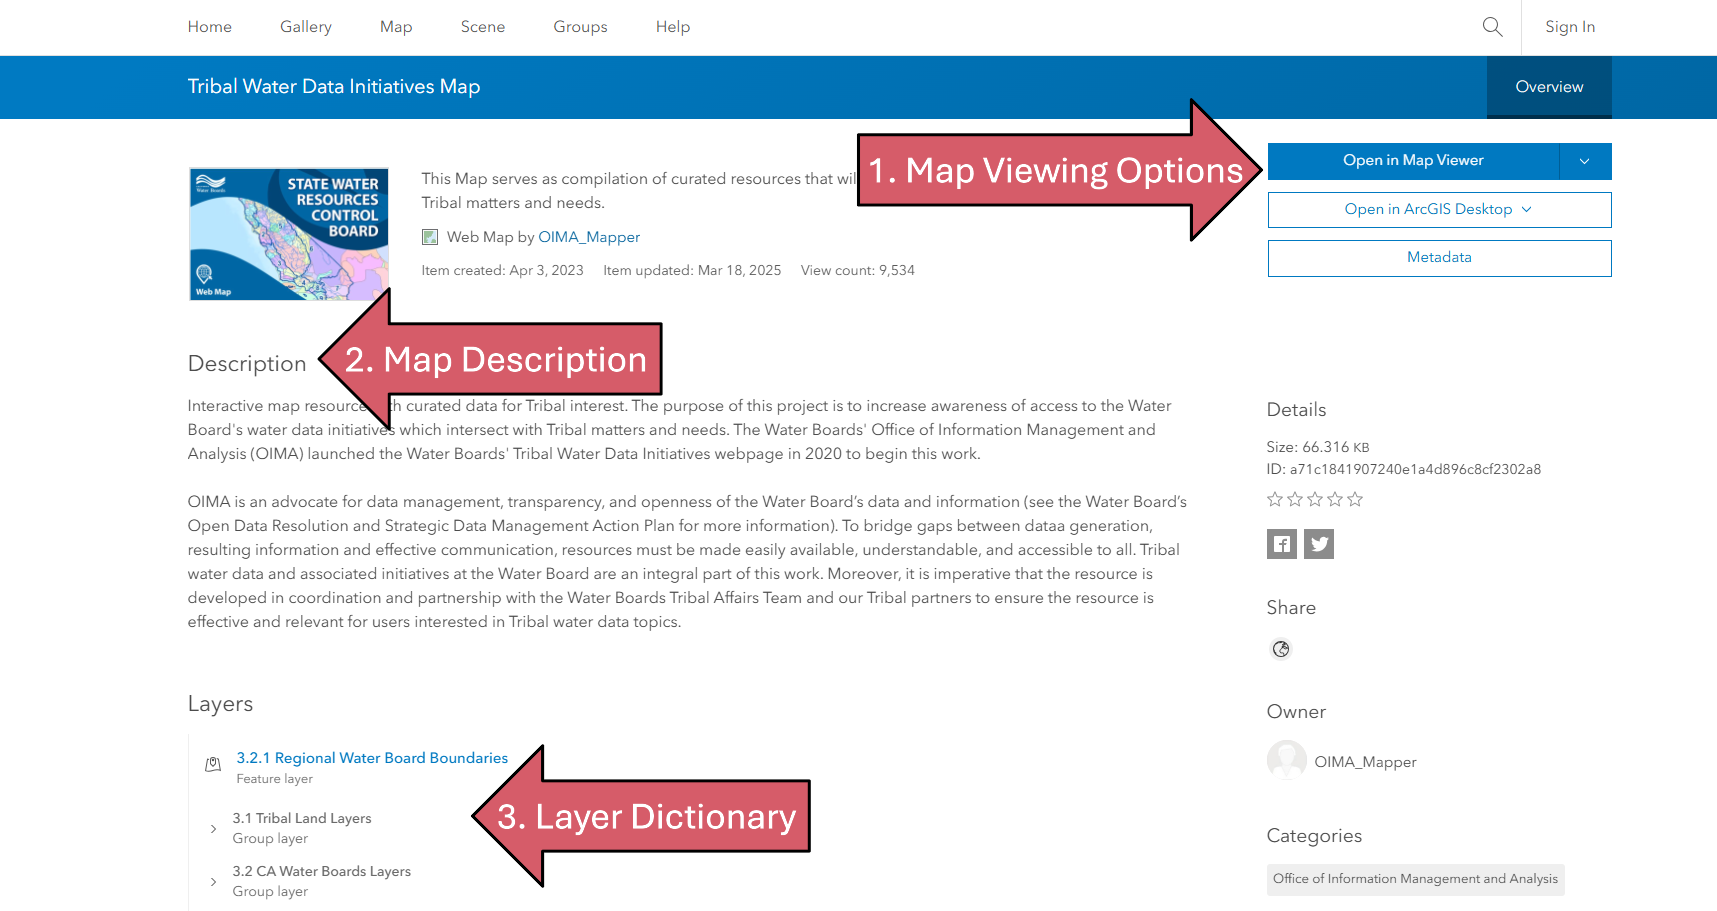
\includegraphics[keepaspectratio]{images/map-guide_open-map.png}}

\section{\texorpdfstring{\textbf{Navigating the
Map}}{Navigating the Map}}\label{navigating-the-map}

After you have clicked on `Open in Map Viewer', the web map will open
with two default layers being displayed: Regional Board Boundaries and
Indigenous Territories.

To navigate the map:

\begin{enumerate}
\def\labelenumi{\arabic{enumi}.}
\item
  To zoom you can use the \textbf{Zoom in}~and~\textbf{Zoom out} buttons
  on the bottom right of map, the mouse and wheel button, or press~Shift
  + Plus Sign~(zoom in) and~Shift + Minus Sign~(zoom out) on the
  keyboard. To zoom in, you can also press the~Shift~key while dragging
  a box on the map.
\item
  To go back to the main view, press the \textbf{house icon}.
\item
  \textbf{Collapse the legend} pane by clicking on the arrow on the
  upper-right corner of the menu.
\item
  Scroll through the \textbf{map options} in the sidebar on the left

  \begin{itemize}
  \tightlist
  \item
    Map options include Layers, Tables and Charts, viewing the BaseMap,
    Viewing the Map Properties, and more.
  \item
    To expand the map options to see icons and words, click on the
    `\textgreater\textgreater{}' arrows in the bottom lefthand corner
    (see Navigating Legend and Layers section below for picture).
  \end{itemize}
\item
  To \textbf{pan the map}, use the mouse or the arrow keys on your
  keyboard.~
\item
  If you're using a Mac with OS X 10.6 or later, you can use multitouch
  gestures by dragging two fingers to pan and zoom the map. The default
  behavior is to pan. To zoom in or out, press~Shift~while dragging two
  fingers toward you to zoom in or dragging two fingers away from you to
  zoom out.
\end{enumerate}

\pandocbounded{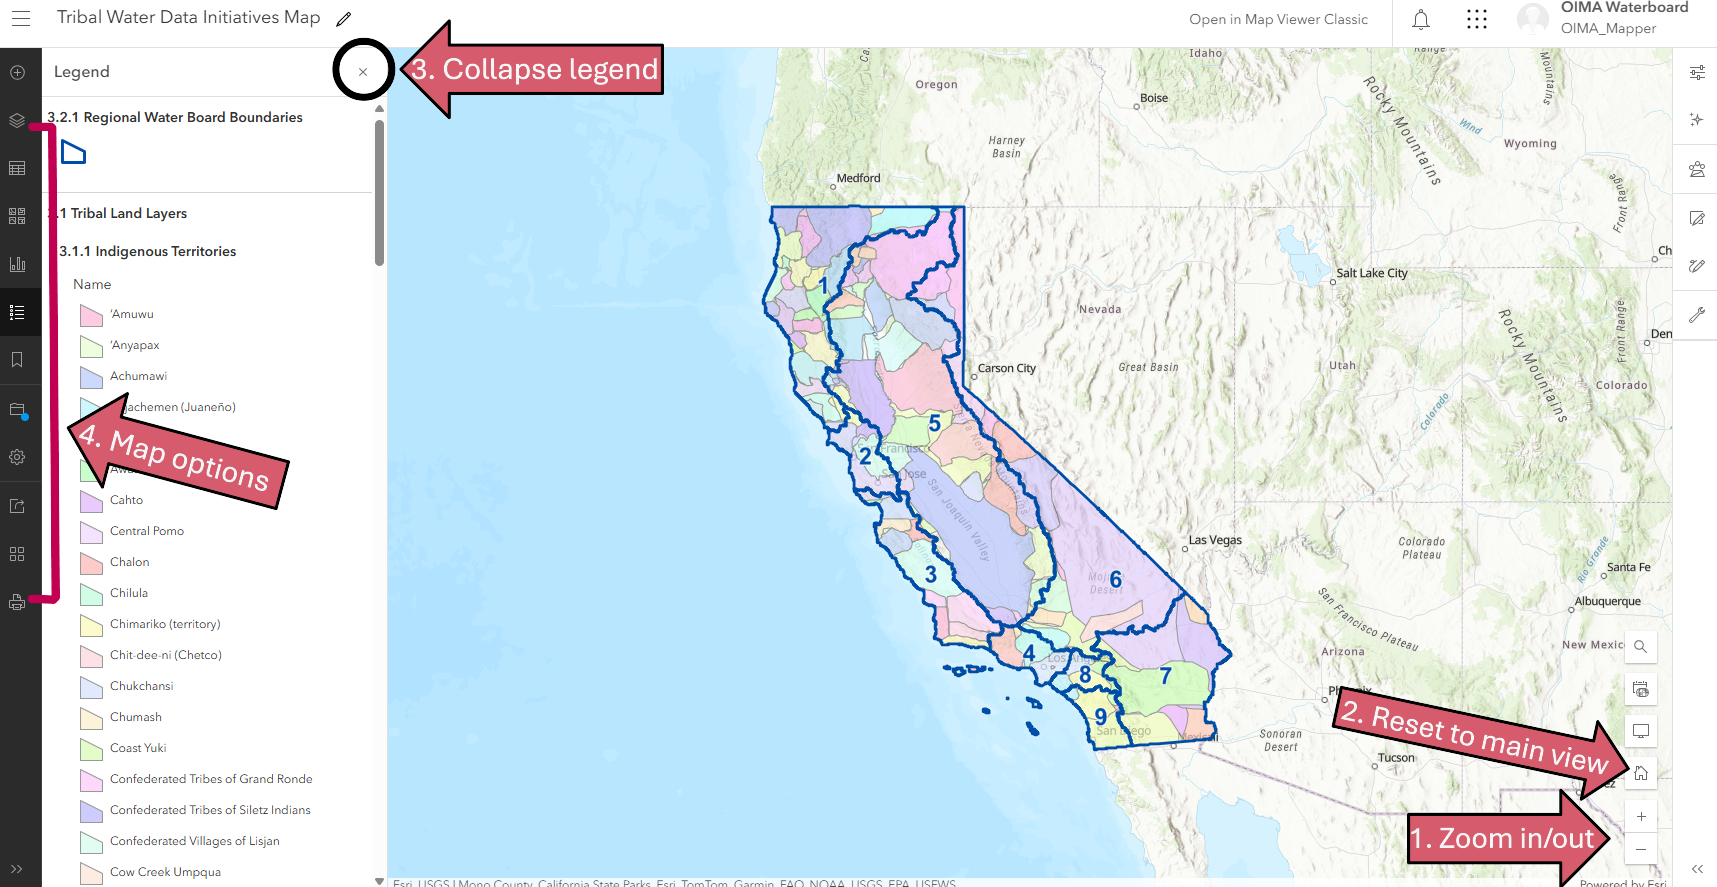
\includegraphics[keepaspectratio]{images/map-guide_navigate-map.png}}

\section{\texorpdfstring{\textbf{Navigating Legend and
Layers}}{Navigating Legend and Layers}}\label{navigating-legend-and-layers}

\begin{itemize}
\item
  To see information on the map, click on any of the items in the
  \textbf{menu bar} on the left side of the screen. For example, to view
  other layers you can click on the \textbf{Layers} icon, which is
  displayed directly to the right of the menu bar.
\item
  Also in the menu bar, is the \textbf{legend} (shown in the inset below
  the pop-up menu). The legend gives more details about each layer that
  is currently selected. For example, the blue outlines and numbers are
  the Regional Board Boundaries and Designations, and the different
  Indigenous Territories are color coded and defined on that menu.
\item
  You can also click on a map area of California to find out what
  Regional Board, or Indigenous Territory is in a specific location. The
  information will be shown in a \textbf{pop-up menu}.

  \begin{itemize}
  \tightlist
  \item
    In this example, the right border of California was clicked and a
    pop-up showed that the area belongs to Region 6 of the Regional
    Boards.
  \end{itemize}
\item
  \textbf{Additional map properties} for exploration and analysis can be
  found on the panel on the right side of the screen for map properties
  and effects, to add a sketch, or to use measurement tools.
\end{itemize}

\pandocbounded{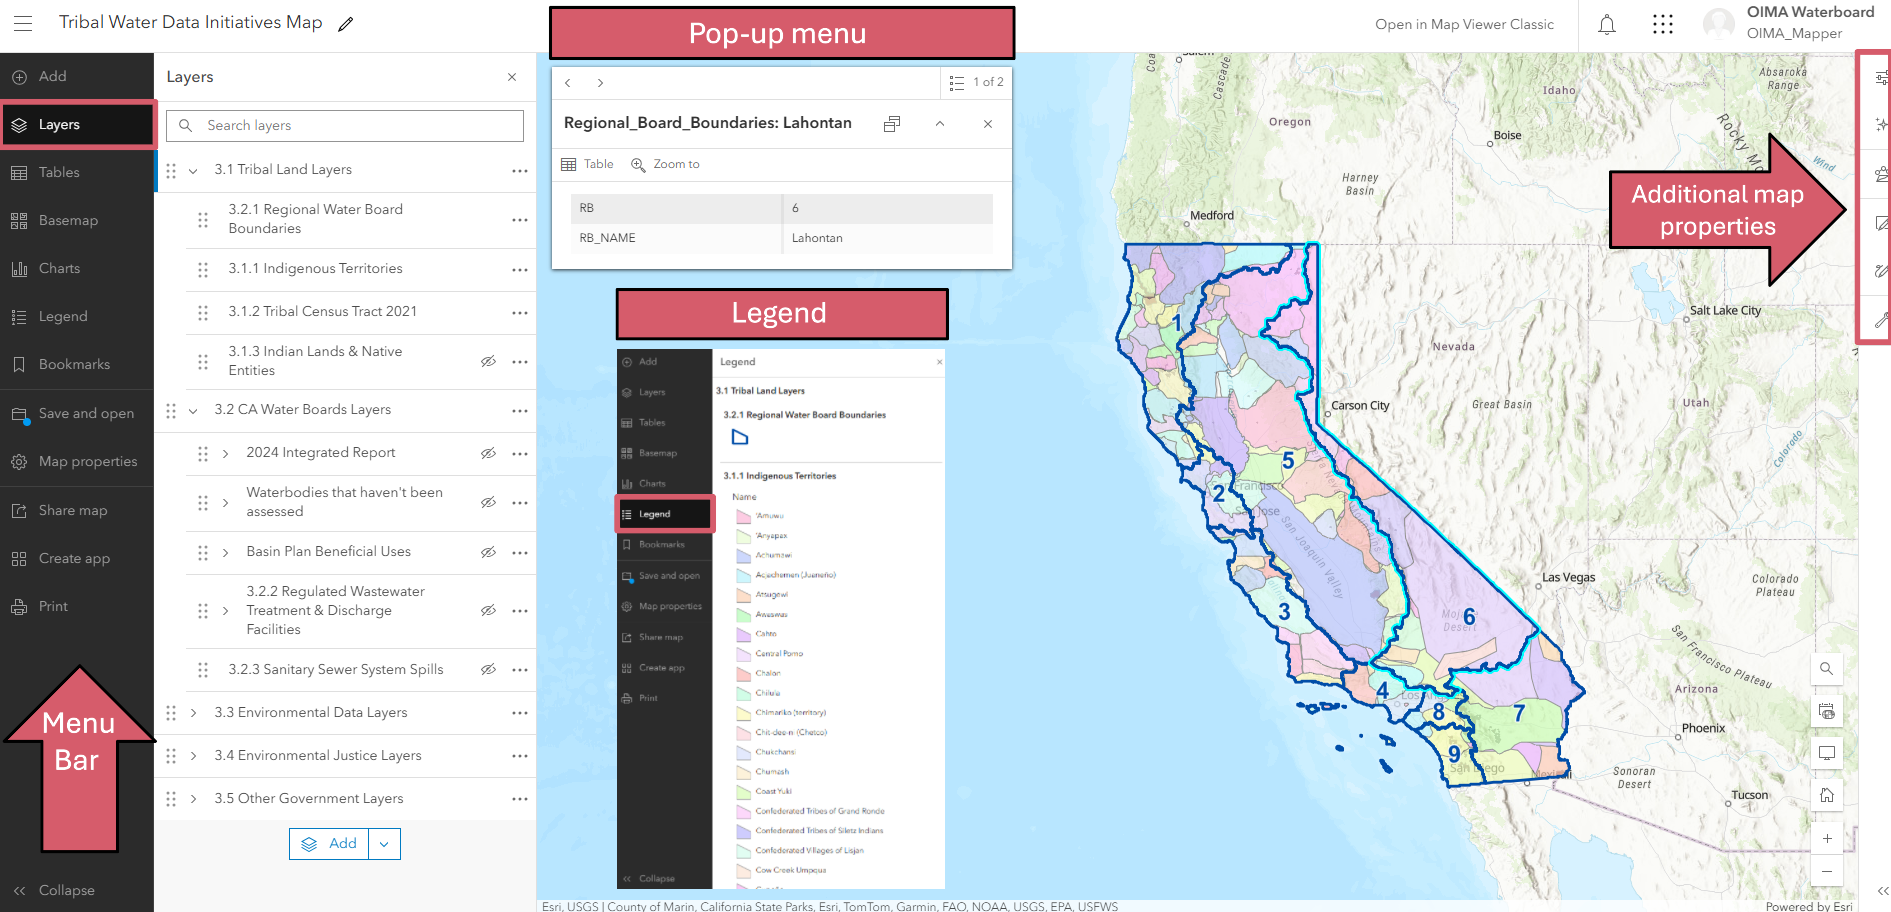
\includegraphics[keepaspectratio]{images/map-guide_navigate-layers.png}}

\section{\texorpdfstring{\textbf{Displaying/Removing View of
Layers}}{Displaying/Removing View of Layers}}\label{displayingremoving-view-of-layers}

\begin{itemize}
\item
  On the \textbf{Menu Bar}, click \textbf{Layers} . All the layers of
  the map will be listed (but not yet displayed). The layer categories
  (3.1, 3.2, 3.3, 3.4, 3.5, and 3.6) are coordinated with the section in
  the
  \href{https://cawaterboarddatacenter.github.io/tribal-water-data-map-manual/layer-guide.html}{Layer
  Guide} that outlines each layer and its important/relevant
  information.
\item
  Upon opening the map, only Regional Boards Boundaries and Indigenous
  Territories will be displayed. You can confirm this by looking at the
  layer name and seeing an eye icon (you may need to hover over the
  layer to see the eye icon). If the eye icon has a slash through it,
  that means the layer is \ul{not} currently visible on the map. You
  need to click on the eye icon specifically to display/remove the
  layer.

  \begin{itemize}
  \tightlist
  \item
    If you just click the layer name and not the eye icon, you will pull
    up the \textbf{properties} information about that layer on the right
    side of the map (shown on the right hand side for Tribal Census
    Tract 2021 layer).
  \end{itemize}
\end{itemize}

\pandocbounded{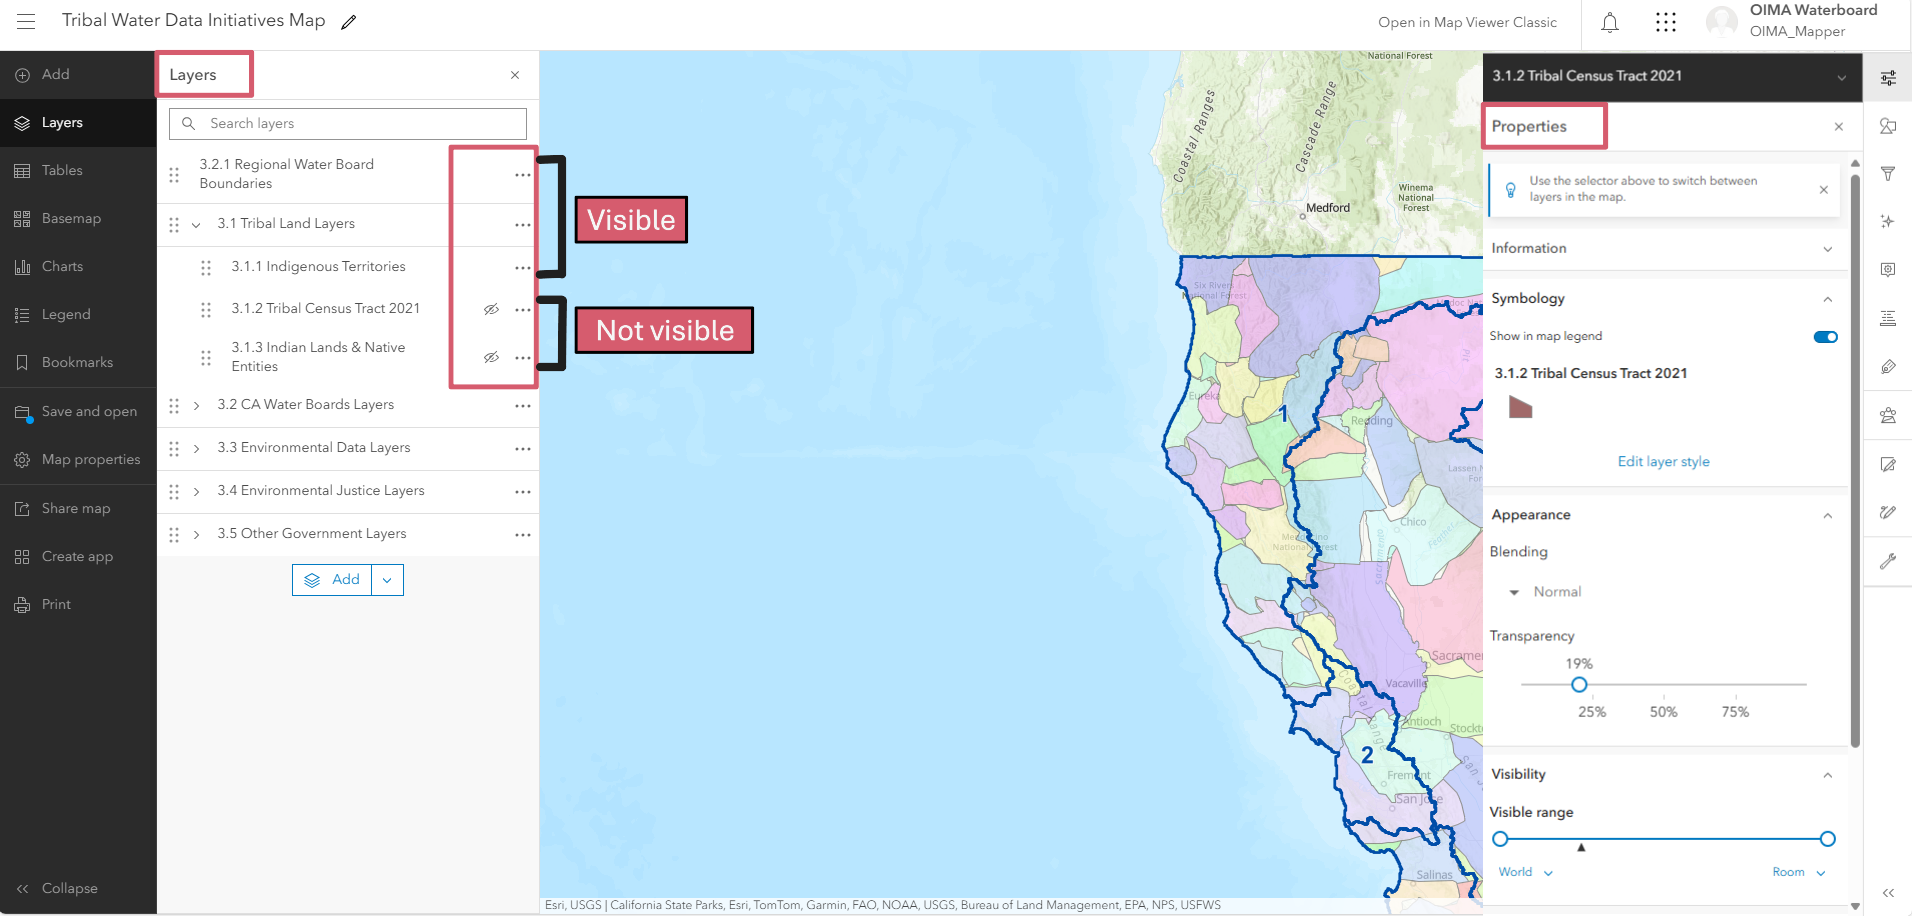
\includegraphics[keepaspectratio]{images/map-guide_content-pane.png}}

\section{\texorpdfstring{\textbf{Adjusting Layer
Transparency}}{Adjusting Layer Transparency}}\label{adjusting-layer-transparency}

To change the transparency of the layers:

\begin{itemize}
\item
  Select the layer of which you'd like to change the transparency:

  \begin{itemize}
  \item
    You can either click on the three dots next to the layer name and
    select ``Show properties'' \ul{or}
  \item
    You can click on the layer name and the properties panel will pop up
    on the right side of the screen.
  \end{itemize}
\item
  Scroll down to \textbf{Appearance}
\item
  Select \textbf{Transparency}, and slide the button to the desired
  transparency

  \begin{itemize}
  \tightlist
  \item
    The more transparency, the less visible the layer will be.
  \end{itemize}
\end{itemize}

\pandocbounded{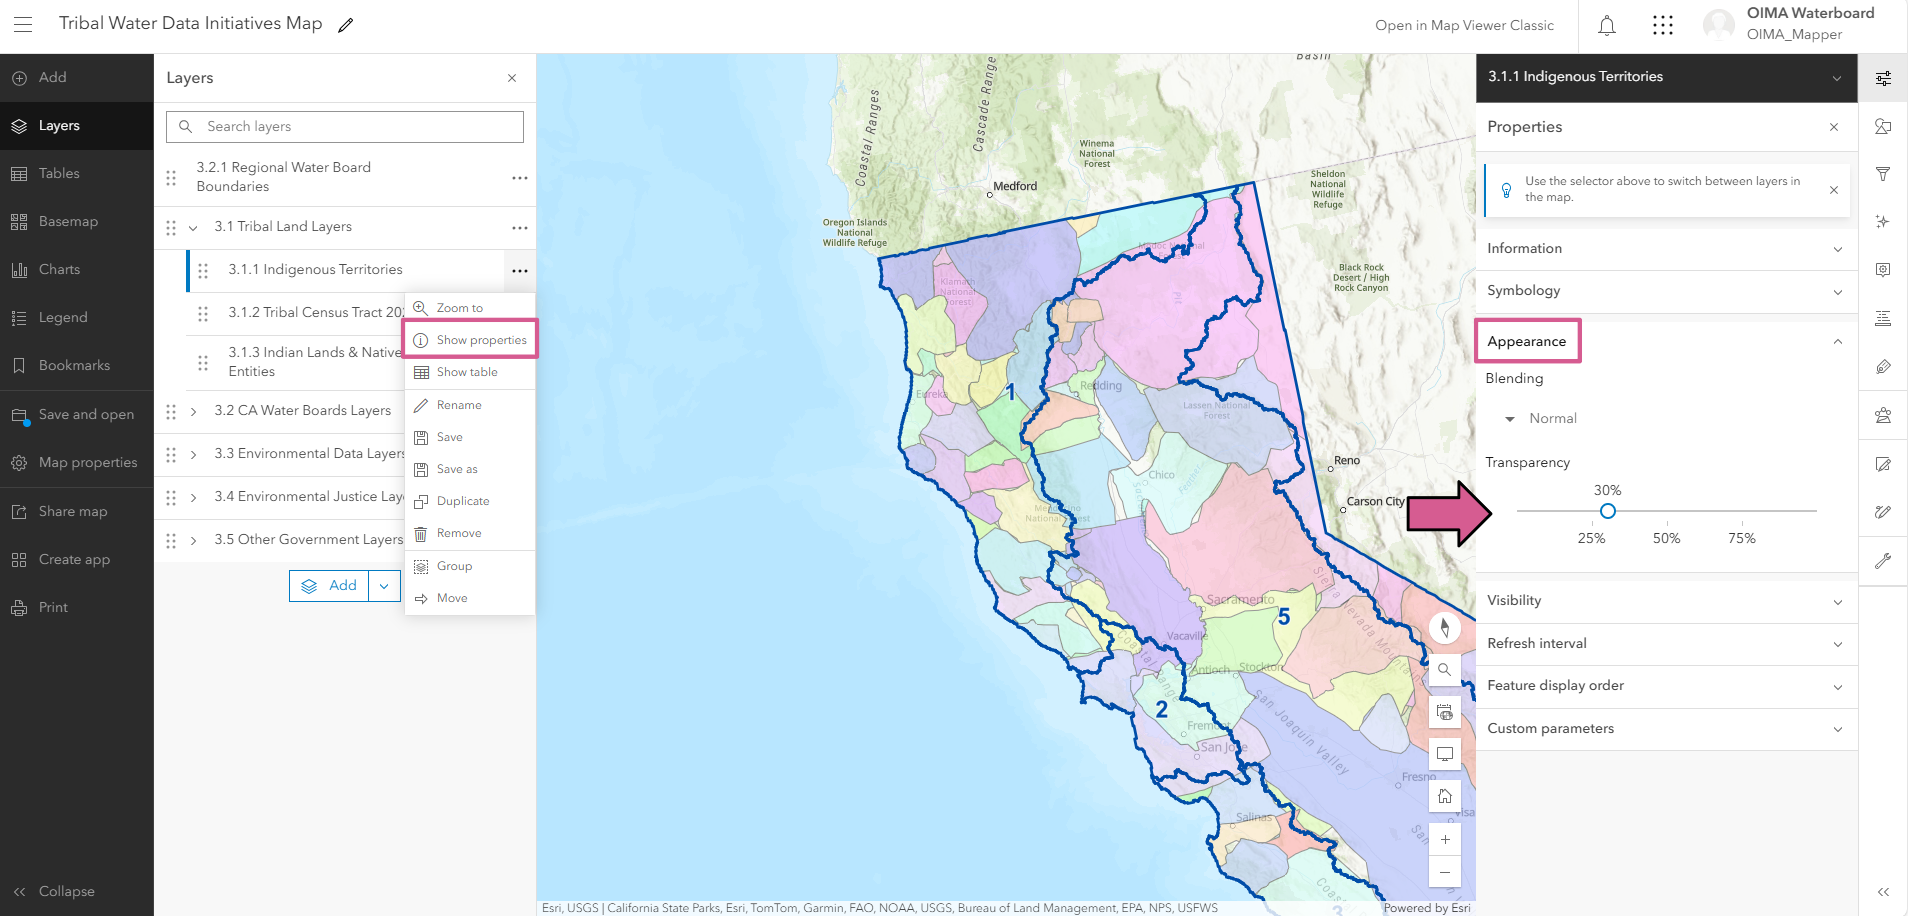
\includegraphics[keepaspectratio]{images/map-guide_transparency.png}}

\bookmarksetup{startatroot}

\chapter{Layer Guide}\label{layer-guide}

This guide serves to provide greater detail about each layer included in
the Tribal Water Data Map.

\begin{tcolorbox}[enhanced jigsaw, breakable, title=\textcolor{quarto-callout-note-color}{\faInfo}\hspace{0.5em}{Note on default map settings}, coltitle=black, colframe=quarto-callout-note-color-frame, opacitybacktitle=0.6, colback=white, opacityback=0, bottomrule=.15mm, colbacktitle=quarto-callout-note-color!10!white, leftrule=.75mm, bottomtitle=1mm, toptitle=1mm, toprule=.15mm, left=2mm, titlerule=0mm, arc=.35mm, rightrule=.15mm]

When opening the map in Map Viewer, the \textbf{default} layers that
will be displayed include all 7 (seven) of the Bureau of Indian Affairs
layers and the California Regional Boards Boundaries. To see more
details about these layers, read below or click on the layer in the
\href{https://gispublic.waterboards.ca.gov/portal/home/item.html?id=16e2736dbf924effbbab3c771bf569fd}{Layer
Dictionary} (see instructions on
\href{https://cawaterboarddatacenter.github.io/tribal-water-data-map-manual/map-guide.html}{Map
Guide} page)

\end{tcolorbox}

\section{Tribal Land Layers}\label{tribal-land-layers}

\subsection{Bureau of Indian Affairs
(BIA)}\label{bureau-of-indian-affairs-bia}

Layer displaying areas of XXXX .

Source:
\href{https://www.bia.gov/sites/default/files/dup/assets/bia/pacreg/PRO_Indian_Lands.gdb_.zip}{Bureau
of Indian Affairs}, from the
\href{https://www.bia.gov/regional-offices/pacific}{Pacific Regional
Office} (PRO)

Data Update Frequency: As needed

Last Updated: June 29th, 2021, added to Tribal Water Data Map in May
2025

Contact: \href{https://www.bia.gov/bia}{BIA}

\href{https://www.bia.gov/bia}{BIA's} mission is to ``enhance the
quality of life, promote economic opportunities, and to carry out the
federal responsibilities entrusted to us to protect and improve the
trust assets of American Indians and Alaska Natives. We accomplish this
by directly empowering Tribal governments through self-governance
agreements.''

\subsubsection{Bureau\_of\_Land\_Management\_Lots}\label{bureau_of_land_management_lots}

This sublayers includes data about Bureau of Land Management (BLM) lands
that are managed within the boundaries of BIA lands.

\emph{screenshot here - layer not appearing}

\subsubsection{Indian\_Lands}\label{indian_lands}

``The term ``Indian land'' means: (A) Any land located within the
boundaries of an Indian reservation, pueblo, or rancheria; (B) Any land
not located within the boundaries of an Indian reservation, pueblo, or
rancheria, the title to which is help: (i) In trust by the United States
for the benefit of an Indian tribe or an individual Indian; (ii) By an
Indian tribe or an individual Indian, subject to restriction against
alienation under laws of the United States Definition: Indian land from
25 USC § 3501(2) \textbar{} LII / Legal Information Institute'',
\href{https://catalog.data.gov/dataset/bia-tract-viewer-ca86a}{BIA Tract
Viewer - Catalog}

\pandocbounded{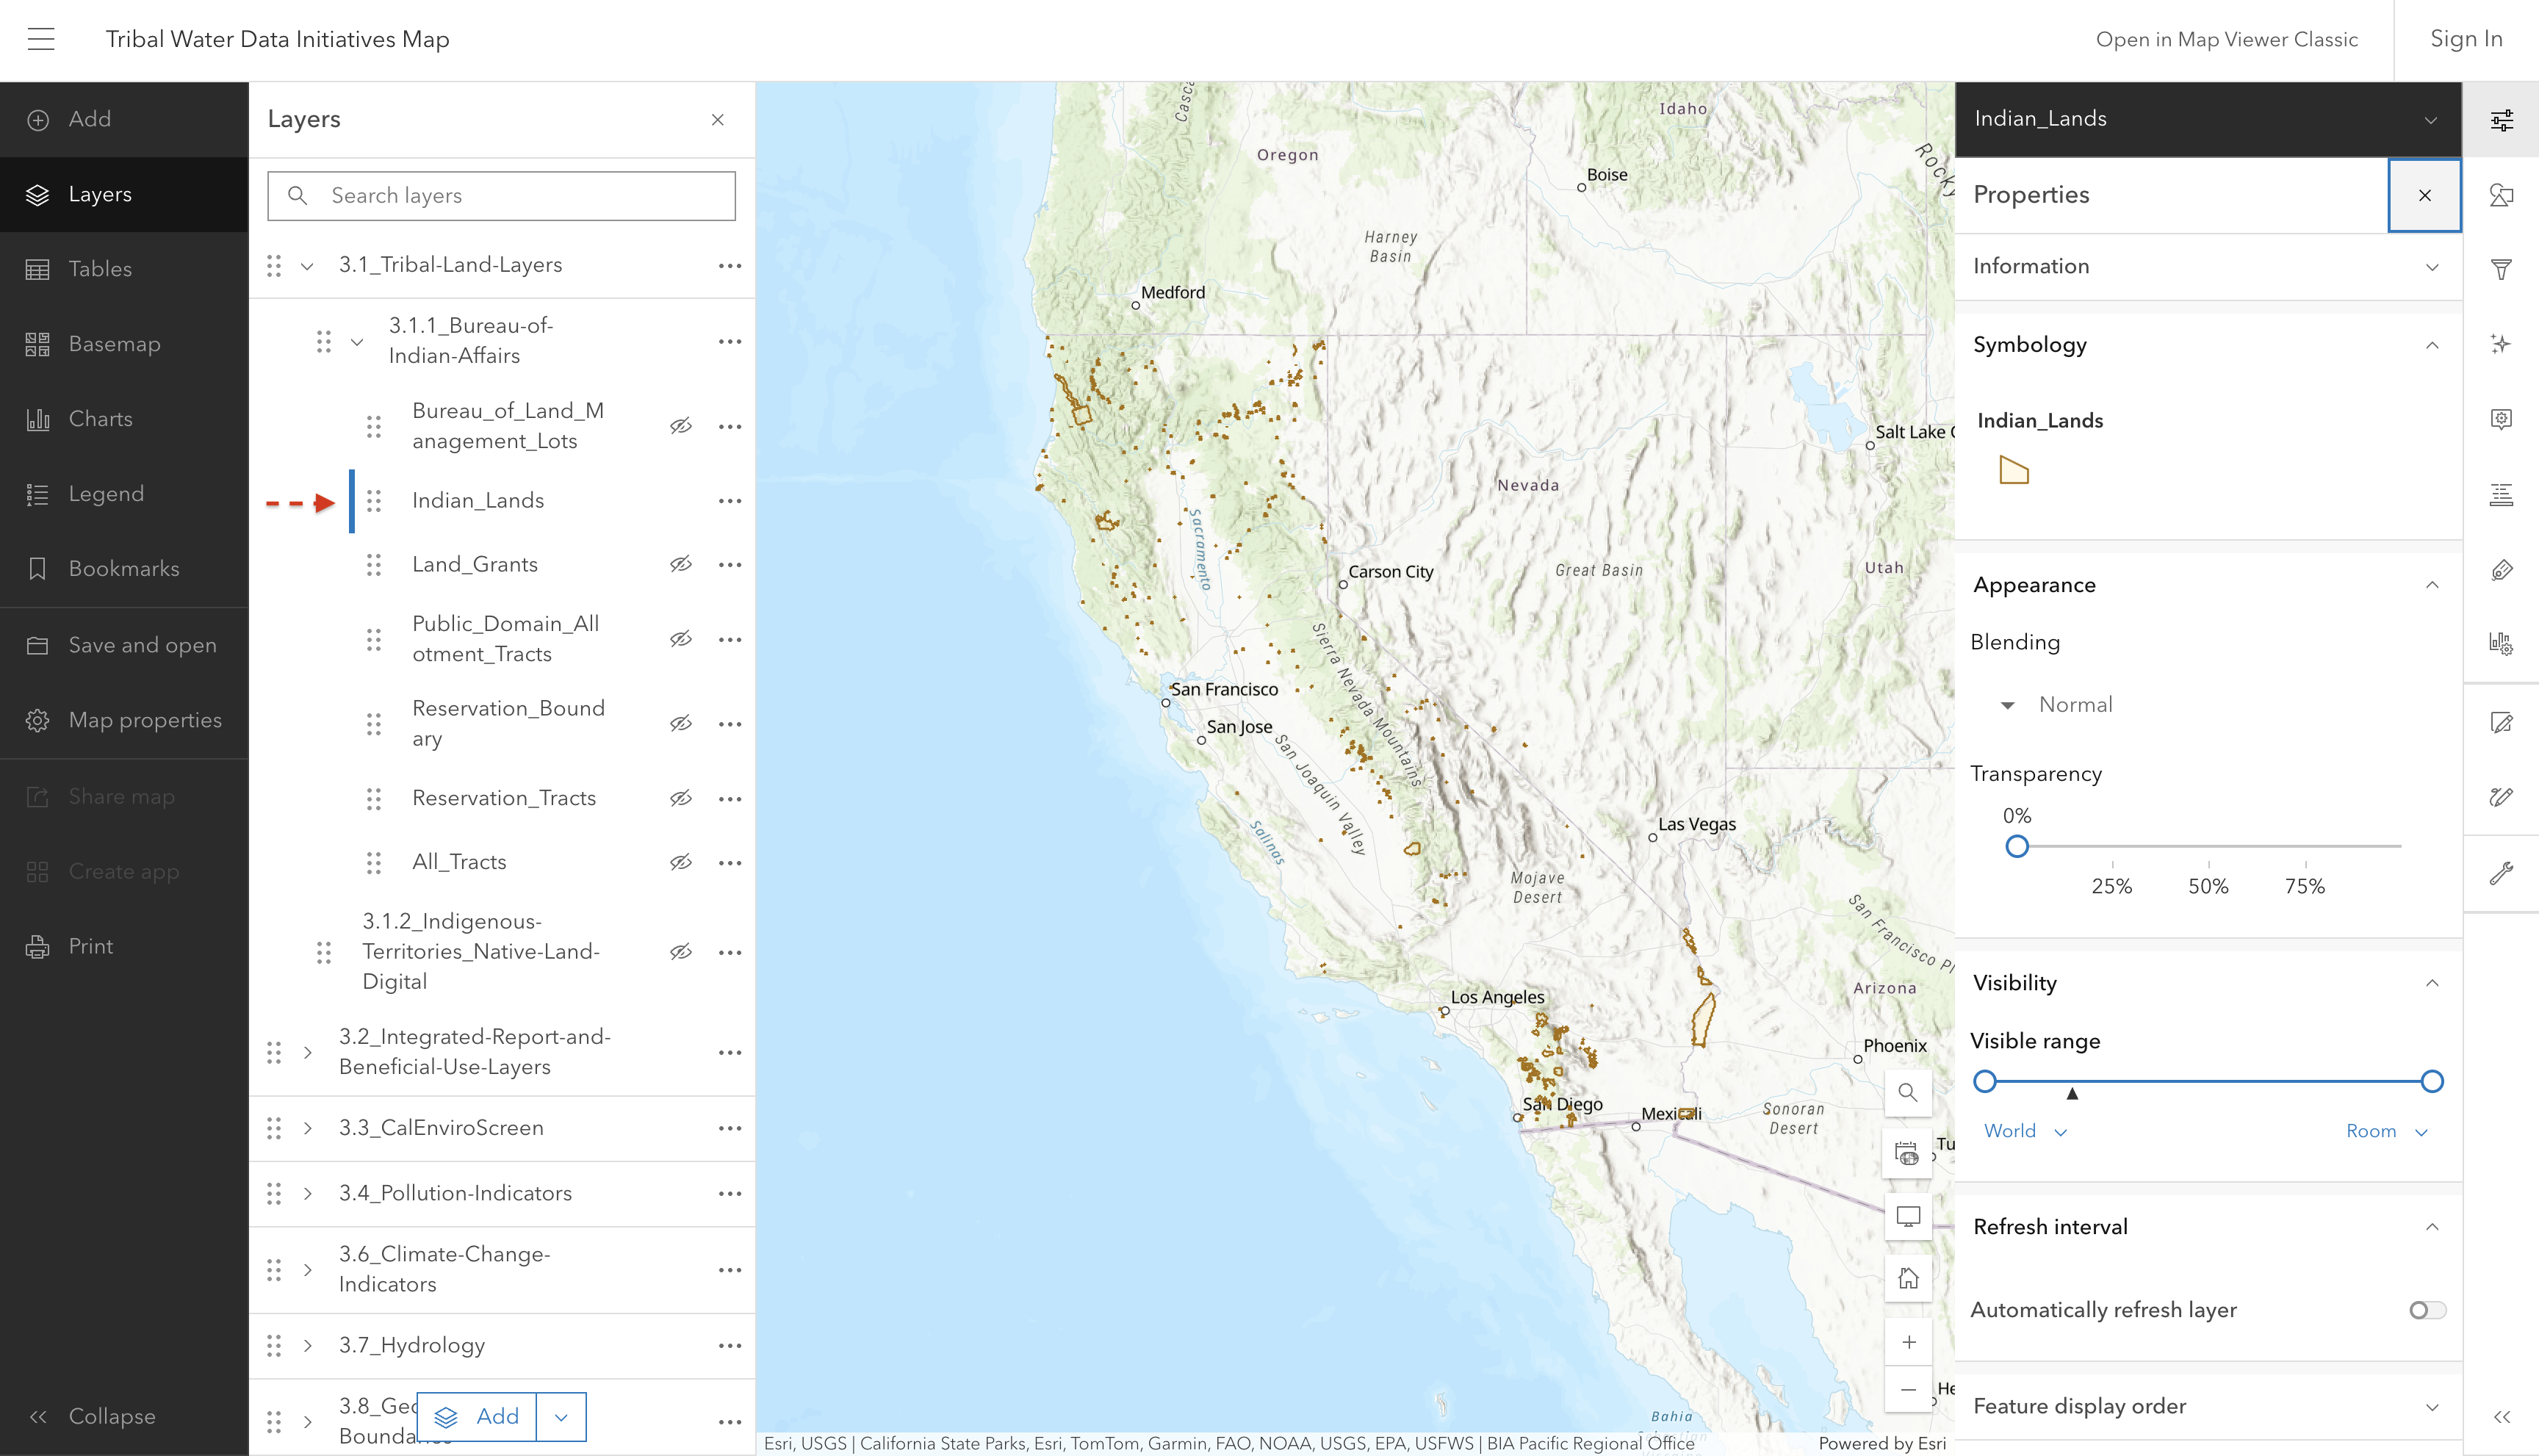
\includegraphics[keepaspectratio]{images/layer-guide_indian-lands.png}}

\subsubsection{Land\_Grants}\label{land_grants}

\emph{screenshot here}

\subsubsection{Public\_Domain\_Allotment\_Tracts}\label{public_domain_allotment_tracts}

These are parcels of Tribal lands, typically up to 160 acres, that were
divided up and ``allotted'' to individual Tribal members, see:
\href{https://www.bia.gov/bia/history/history-indian-land-consolidation\#:~:text=In\%201887\%2C\%20Congress\%20enacted\%20the,allotted\%E2\%80\%9D\%20to\%20individual\%20Tribal\%20members.}{Allotment
Act of 1887}.~

\emph{screenshot here}

\subsubsection{Reservation\_Boundary}\label{reservation_boundary}

This sublayer refers to the outer limits or perimeter of federal
American Indian reservations.~These boundaries are established by
treaties, agreements, executive orders, or other federal actions and
define the land reserved for a Tribe or Tribes.

\subsubsection{Reservation\_Tracts}\label{reservation_tracts}

\emph{screenshot here}

\subsubsection{All\_Tracts}\label{all_tracts}

\emph{screenshot here}

\subsection{Indigenous Territories}\label{indigenous-territories}

Layer displaying historic Indigenous Territories within California.

Source:
\href{https://gispublic.waterboards.ca.gov/portal/home/item.html?id=c21e3128ad4b4f68b041420c3f19c4c8}{Water
Boards ArcGIS Portal}, data used in this layer was accessed and
downloaded from \href{https://native-land.ca/}{native-land.ca}

Data Update Frequency: As needed

Last Updated: May 2024

Contact: \href{https://native-land.ca/contact}{Native Land Digital}

\href{https://native-land.ca/about/why-it-matters}{Native Land Digital}
``strives to create and foster conversations about the history of
colonialism, Indigenous ways of knowing, and settler-Indigenous
relations, through educational resources such as our map and Territory
Acknowledgement Guide. We strive to go beyond old ways of talking about
Indigenous people and to develop a platform where Indigenous communities
can represent themselves and their histories on their own terms. In
doing so, Native Land Digital creates spaces where non-Indigenous people
can be invited and challenged to learn more about the lands they
inhabit, the history of those lands, and how to actively be part of a
better future going forward together.''

\subsection{Other Sources of American Indian and Tribal
Land}\label{other-sources-of-american-indian-and-tribal-land}

\subsubsection{Tribal Census Tract 2021}\label{tribal-census-tract-2021}

Layer showing Tribal areas identified by the U.S. Census Bureau. You can
zoom in further to see specific areas more closely.

Source:
\href{https://www.census.gov/cgi-bin/geo/shapefiles/index.php?year=2024&layergroup=American+Indian+Area+Geography}{U.S.
Census Bureau},
\href{https://www.census.gov/geographies/mapping-files/time-series/geo/tiger-line-file.html}{TIGER/Line
Shapefiles}

Data Update Frequency: Every 10 years

Last updated: 2024

Contact: \href{https://www.census.gov/about/contact-us.html}{U.S Census
Bureau}

\subsubsection{Tribal and Native
Entities}\label{tribal-and-native-entities}

Layer showing American Indians Reservations/Federally Recognized Tribal
Entities.

Source:
\href{https://calema.maps.arcgis.com/apps/mapviewer/index.html?layers=0b6c3f61f0c04168b2de56ac321ab76d}{California
Governor's Office of Emergency Services (Cal OES)}

Data Update Frequency: As needed

Last updated: 2019

Contact:
\href{https://www.caloes.ca.gov/office-of-the-director/policy-administration/tribal-coordination/}{Cal
OES}

The American Indians Reservations/Federally Recognized Tribal Entities
data set depicts feature location, selected demographics and other
associated data for the 561 Federally Recognized Tribal entities in the
contiguous U.S. and Alaska. Categories included are: American Indian
Reservations (AIR), Federally Recognized Tribal Entities (FRTE) and
Alaska Native Villages (ANV).

\section{Integrated Report and Beneficial Use
Layers}\label{integrated-report-and-beneficial-use-layers}

\subsection{2024 Integrated Report}\label{integrated-report}

\begin{tcolorbox}[enhanced jigsaw, breakable, title=\textcolor{quarto-callout-important-color}{\faExclamation}\hspace{0.5em}{Important}, coltitle=black, colframe=quarto-callout-important-color-frame, opacitybacktitle=0.6, colback=white, opacityback=0, bottomrule=.15mm, colbacktitle=quarto-callout-important-color!10!white, leftrule=.75mm, bottomtitle=1mm, toptitle=1mm, toprule=.15mm, left=2mm, titlerule=0mm, arc=.35mm, rightrule=.15mm]

\textbf{What is the Integrated Report?}

Waterbodies assessed in the Integrated Report (IR) include surface
waterbodies, such as rivers, lakes, and beaches.

Assessed waterbodies are placed into one of five Integrated Report
Condition Categories based on the waterbody's ability to support
beneficial use(s).

The 303(d) list consists of the waterbodies in Categories 4a, 4b, and 5.
These waterbodies can be referred to as ``listed'' or ``impaired''.

\begin{itemize}
\item
  The 303(d) list is based off of Section 303(d) of the Clean Water Act,
  which requires each state to identify waters that do not meet water
  quality standards and to prioritize those waters for development of
  total maximum daily load (TMDL)
\item
  The Clean Water Act also requires each state to report on the overall
  condition of its surface waterbodies, which is Section 305(b).
\end{itemize}

California combines its 303(d) lists and 305(b) reports into a single
``California Integrated Report''.

For more information see:

\href{https://ceden.org/303d_list.shtml}{CEDEN - California
Environmental Data Exchange Network}

\href{https://www.waterboards.ca.gov/water_issues/programs/water_quality_assessment/2024-integrated-report.html}{2024
Integrated Report \textbar{} California State Water Resources Control
Board}

\end{tcolorbox}

\subsubsection{State Water Bodies (rivers, streams, and
beaches)}\label{state-water-bodies-rivers-streams-and-beaches}

This layer shows linear waterbodies in California, such as rivers,
streams, and beaches, which were assessed for 305(b) in the 2022-2024
California Integrated Report. Blue waterbodies are listed in Category 1,
2, or 3. Orange waterbodies represent those placed on the 303(d) list of
impaired waters.

\pandocbounded{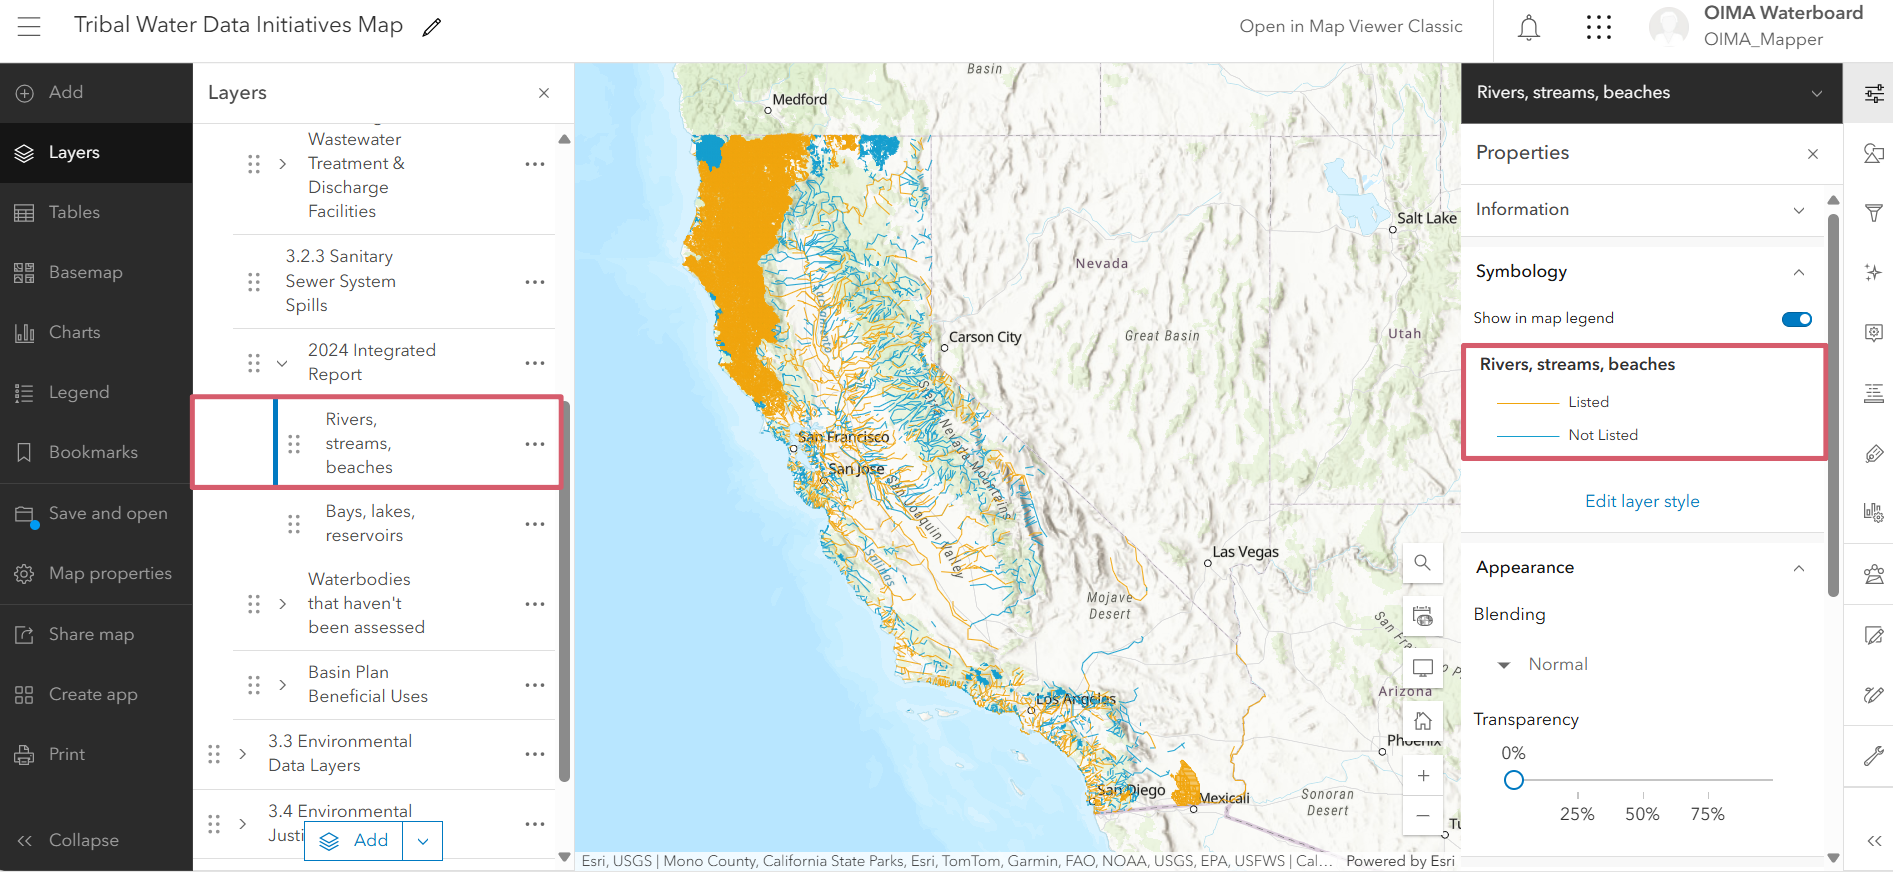
\includegraphics[keepaspectratio]{images/layer-guide_integrated-report-linear.png}}

Note, these are not the final assessments.~

Source:

Data Update Frequency: Every two years

Contact:
\href{https://www.waterboards.ca.gov/water_issues/programs/water_quality_assessment/}{SWRCB
Water Quality Assessment Program}

\subsubsection{State Water Bodies (bays, lakes and
reservoirs)}\label{state-water-bodies-bays-lakes-and-reservoirs}

This layer shows non-linear (polygon) waterbodies in California, such as
bays, lakes, and reservoirs, which were assessed for 305(b) in the
2020-2022 California Integrated Report. Blue waterbodies are listed in
Category 1, 2, or 3. Orange waterbodies represent those placed on the
303(d) list of impaired waters.

\pandocbounded{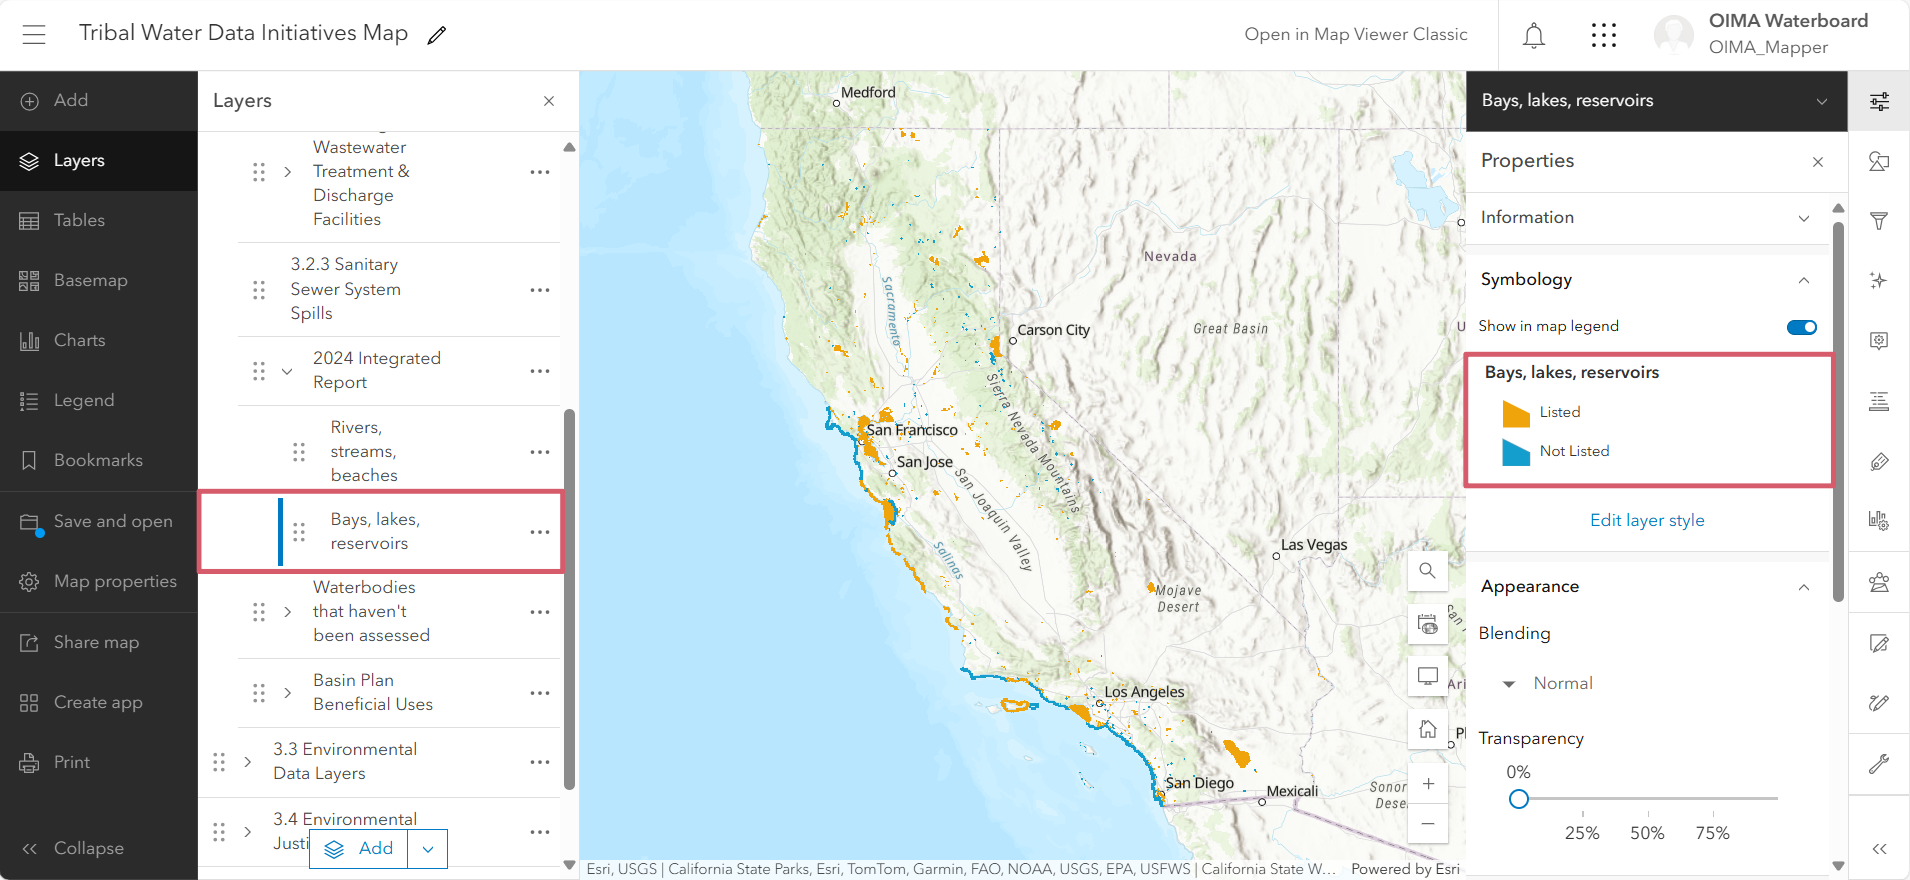
\includegraphics[keepaspectratio]{images/layer-guide_integrated-report-non-linear.png}}

Note, these are not the final assessments.~

Source:

Data Update Frequency: Every 2 years

Contact:
\href{https://www.waterboards.ca.gov/water_issues/programs/water_quality_assessment/}{SWRCB
Water Quality Assessment Program}

\subsection{Waterbodies that haven't been
assessed}\label{waterbodies-that-havent-been-assessed}

\subsubsection{State Water Bodies (rivers, streams, and
beaches)}\label{state-water-bodies-rivers-streams-and-beaches-1}

\pandocbounded{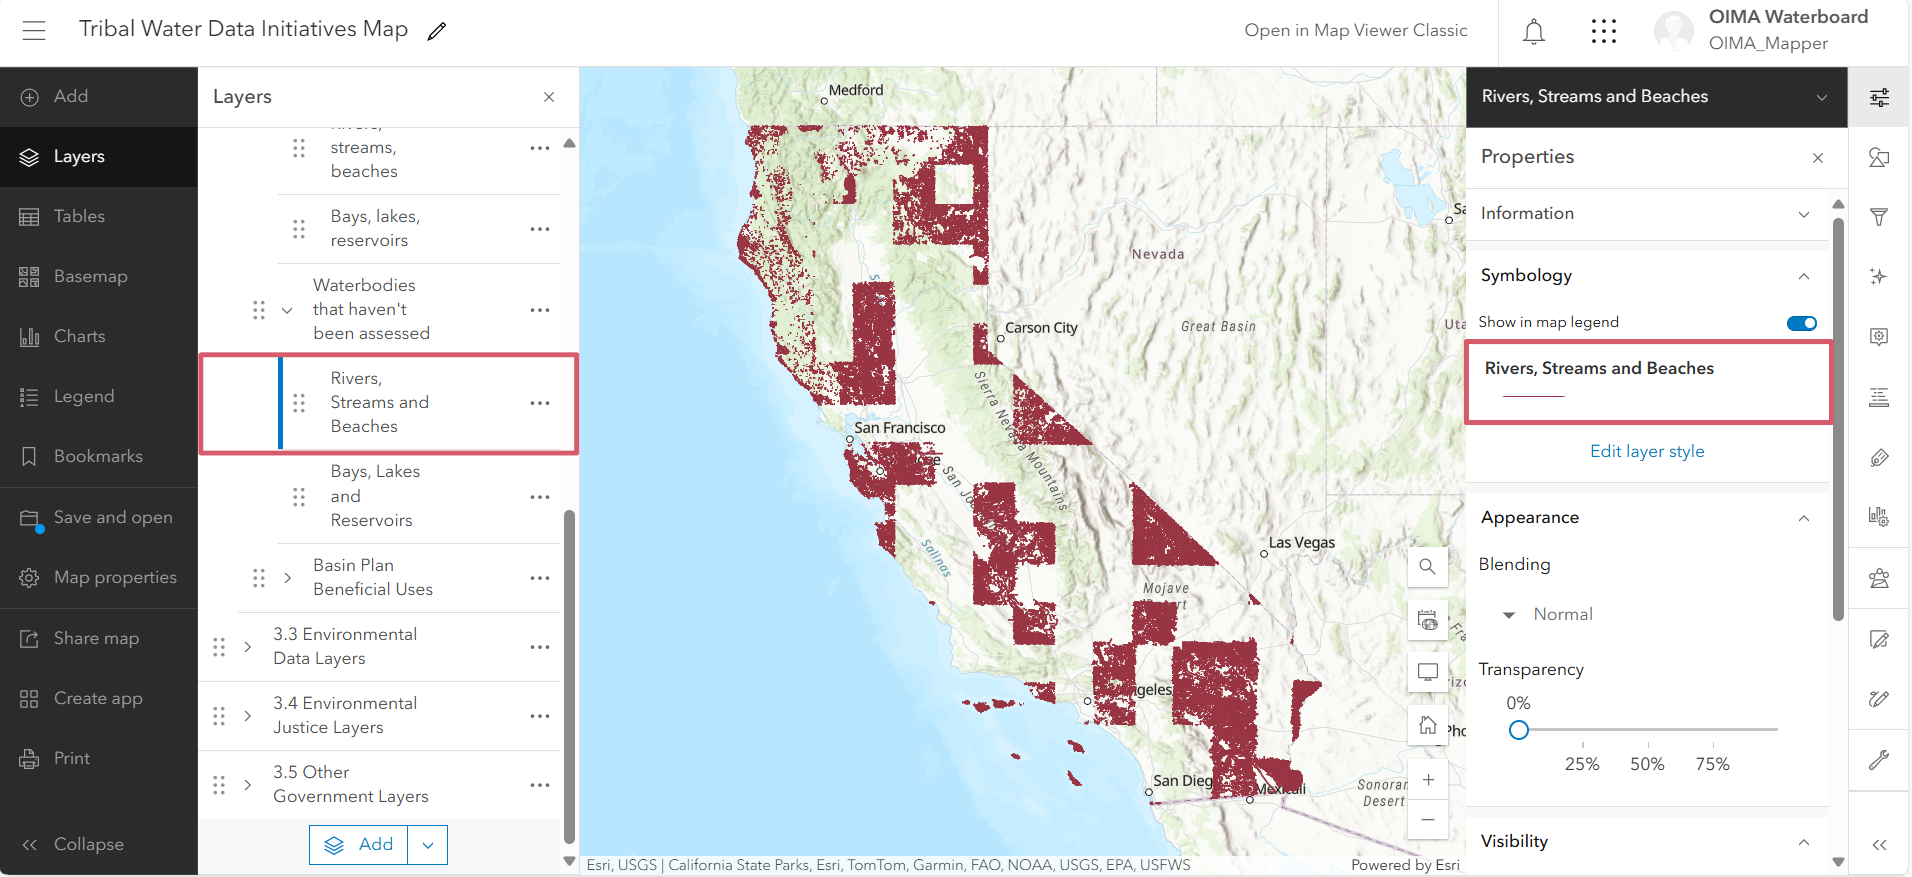
\includegraphics[keepaspectratio]{images/layer-guide_unassessedwaterbodies_rivers.png}}

\subsubsection{State Water Bodies (bays, lakes and
reservoirs)}\label{state-water-bodies-bays-lakes-and-reservoirs-1}

\pandocbounded{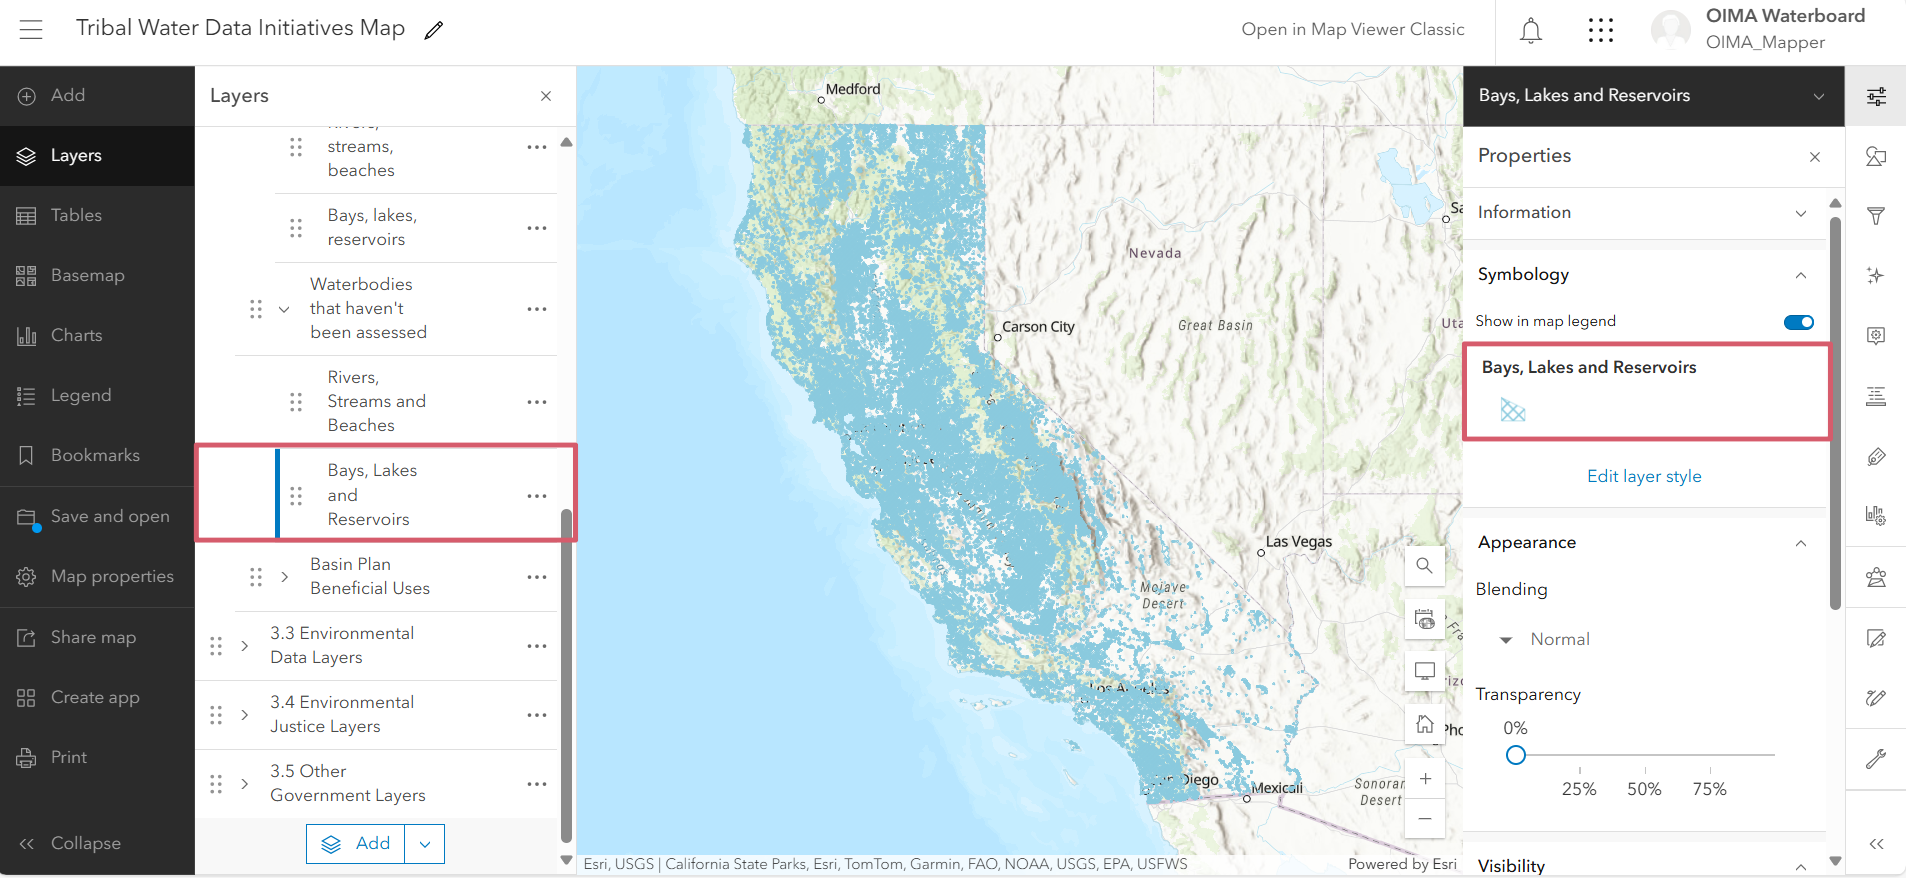
\includegraphics[keepaspectratio]{images/layer-guide-unassessedwaterbodies-bays.png}}

\subsection{Basin Plan Beneficial
Uses}\label{basin-plan-beneficial-uses}

\begin{tcolorbox}[enhanced jigsaw, breakable, title=\textcolor{quarto-callout-important-color}{\faExclamation}\hspace{0.5em}{Important}, coltitle=black, colframe=quarto-callout-important-color-frame, opacitybacktitle=0.6, colback=white, opacityback=0, bottomrule=.15mm, colbacktitle=quarto-callout-important-color!10!white, leftrule=.75mm, bottomtitle=1mm, toptitle=1mm, toprule=.15mm, left=2mm, titlerule=0mm, arc=.35mm, rightrule=.15mm]

\textbf{What are Beneficial Uses?}

\end{tcolorbox}

\subsubsection{State Water Bodies (rivers, streams, and
beaches)}\label{state-water-bodies-rivers-streams-and-beaches-2}

\pandocbounded{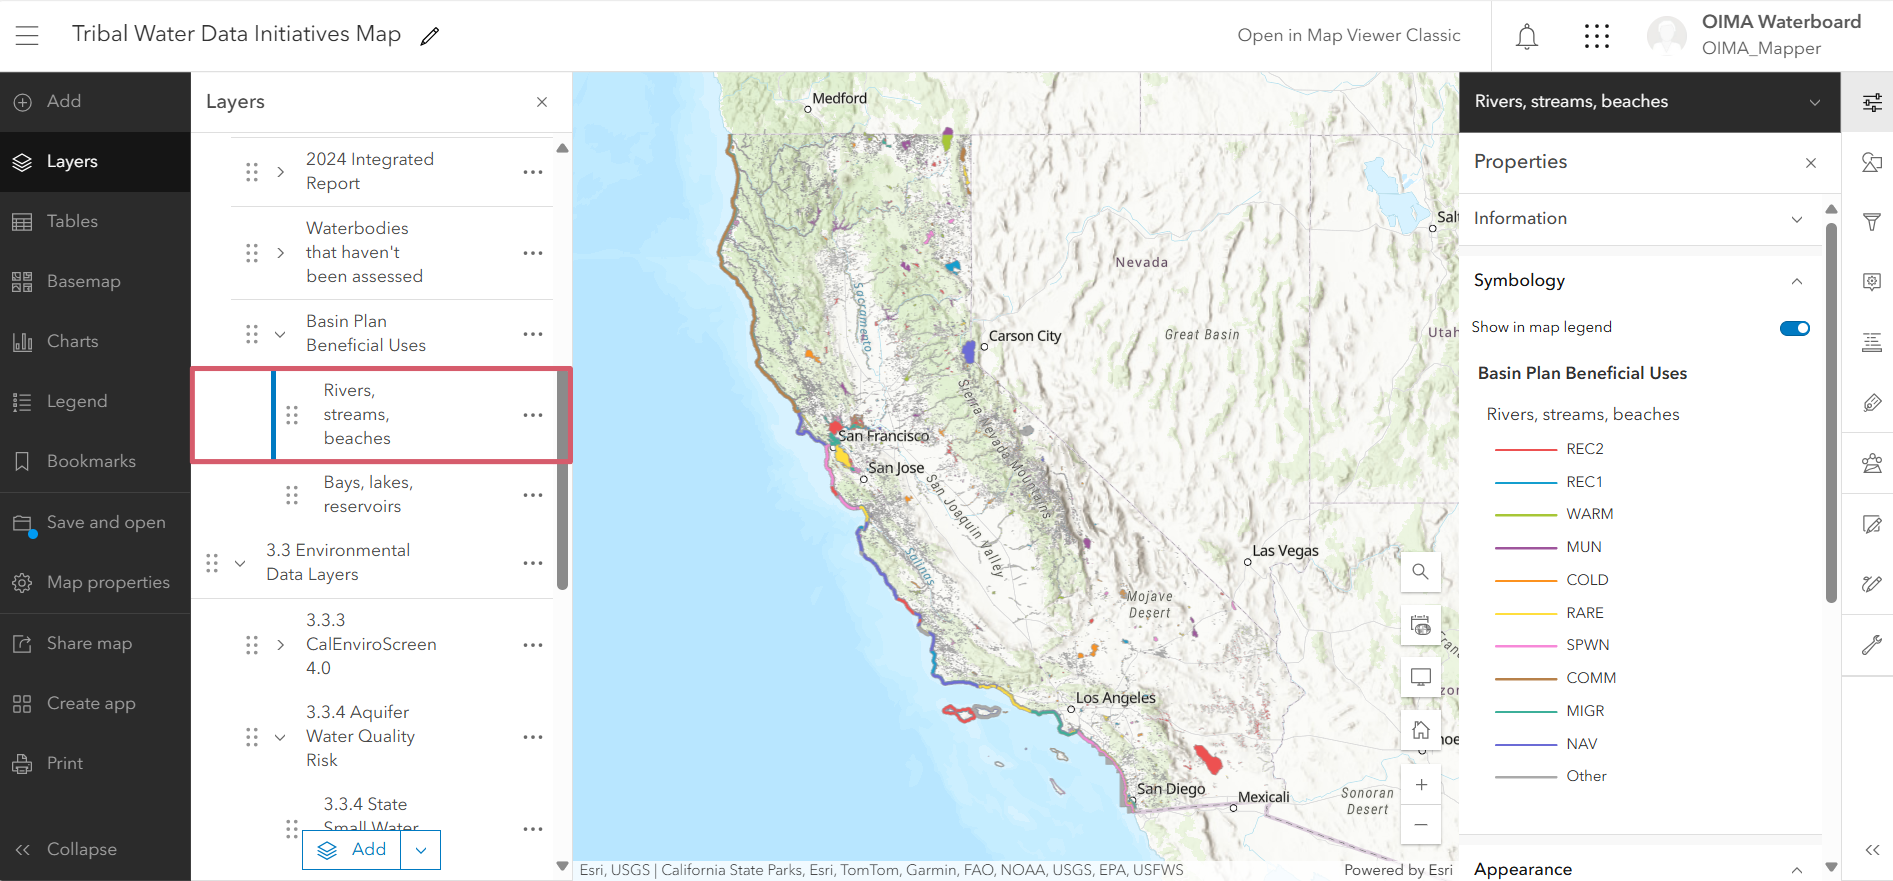
\includegraphics[keepaspectratio]{images/layer-guide_basin-use.png}}

\subsubsection{State Water Bodies (bays, lakes and
reservoirs)}\label{state-water-bodies-bays-lakes-and-reservoirs-2}

\section{CalEnviroScreen}\label{calenviroscreen}

\subsection{CalEnviroScreen 4.0}\label{calenviroscreen-4.0}

This layer shows the CalEnviroScreen (CES) 4.0 based on the CES Score
percentile.

CalEnviroScreen is a screening methodology that can be used to help
identify California communities that are disproportionately burdened by
multiple sources of pollution. CI score ranges from 10 to 100. For more
information on CalEnviroScreen scoring, see Practice Examples page.

\pandocbounded{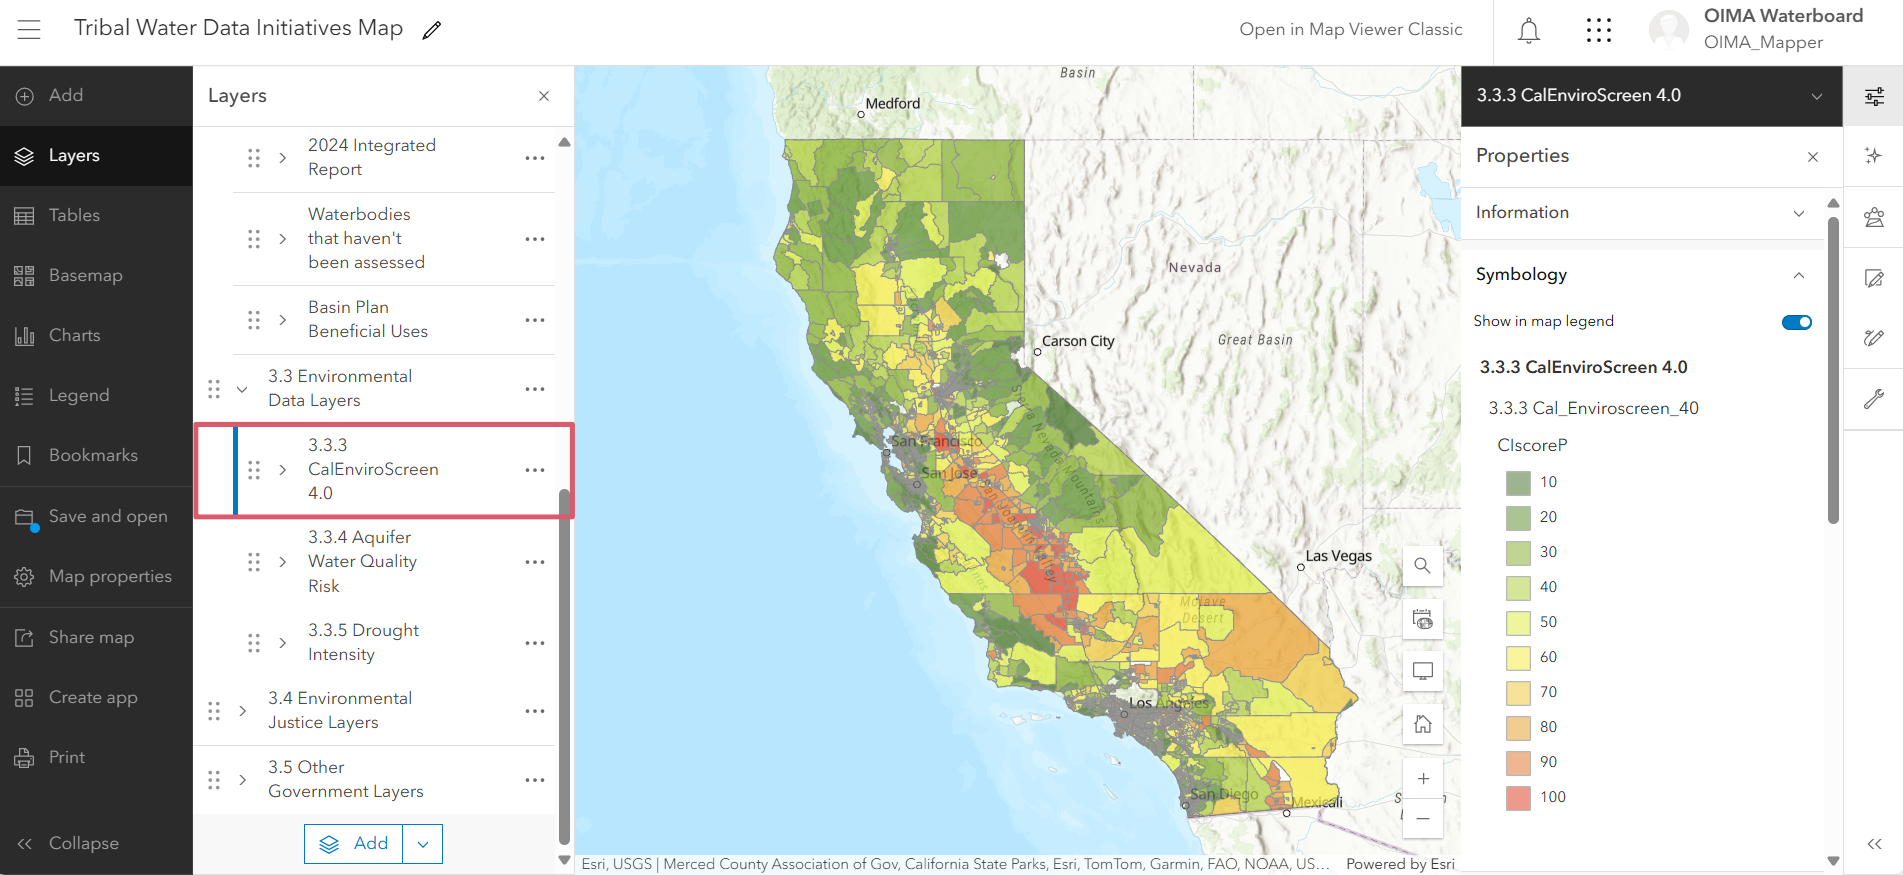
\includegraphics[keepaspectratio]{images/layer-guide_cal-enviro-screen.png}}

Source:
\href{https://oehha.ca.gov/calenviroscreen/report/calenviroscreen-40}{California
Office of Environmental Health Hazard Assessment (OEHHA)}

Data Update Frequency: As needed

Contact:
\href{https://oehha.ca.gov/calenviroscreen/contact-calenviroscreen}{CalEnviroScreen}

\subsection{Disadvantaged Communities}\label{disadvantaged-communities}

This map shows the disadvantaged communities designated by CalEPA for
the purpose of SB 535. These areas represent the 25\% highest scoring
census tracts in CalEnviroScreen 4.0, census tracts previously
identified in the top 25\% in CalEnviroScreen 3.0, census tracts with
high amounts of pollution and low populations, and federally recognized
tribal areasas identified by the Census in the 2021 American Indian
Areas Related National Geodatabase.

\pandocbounded{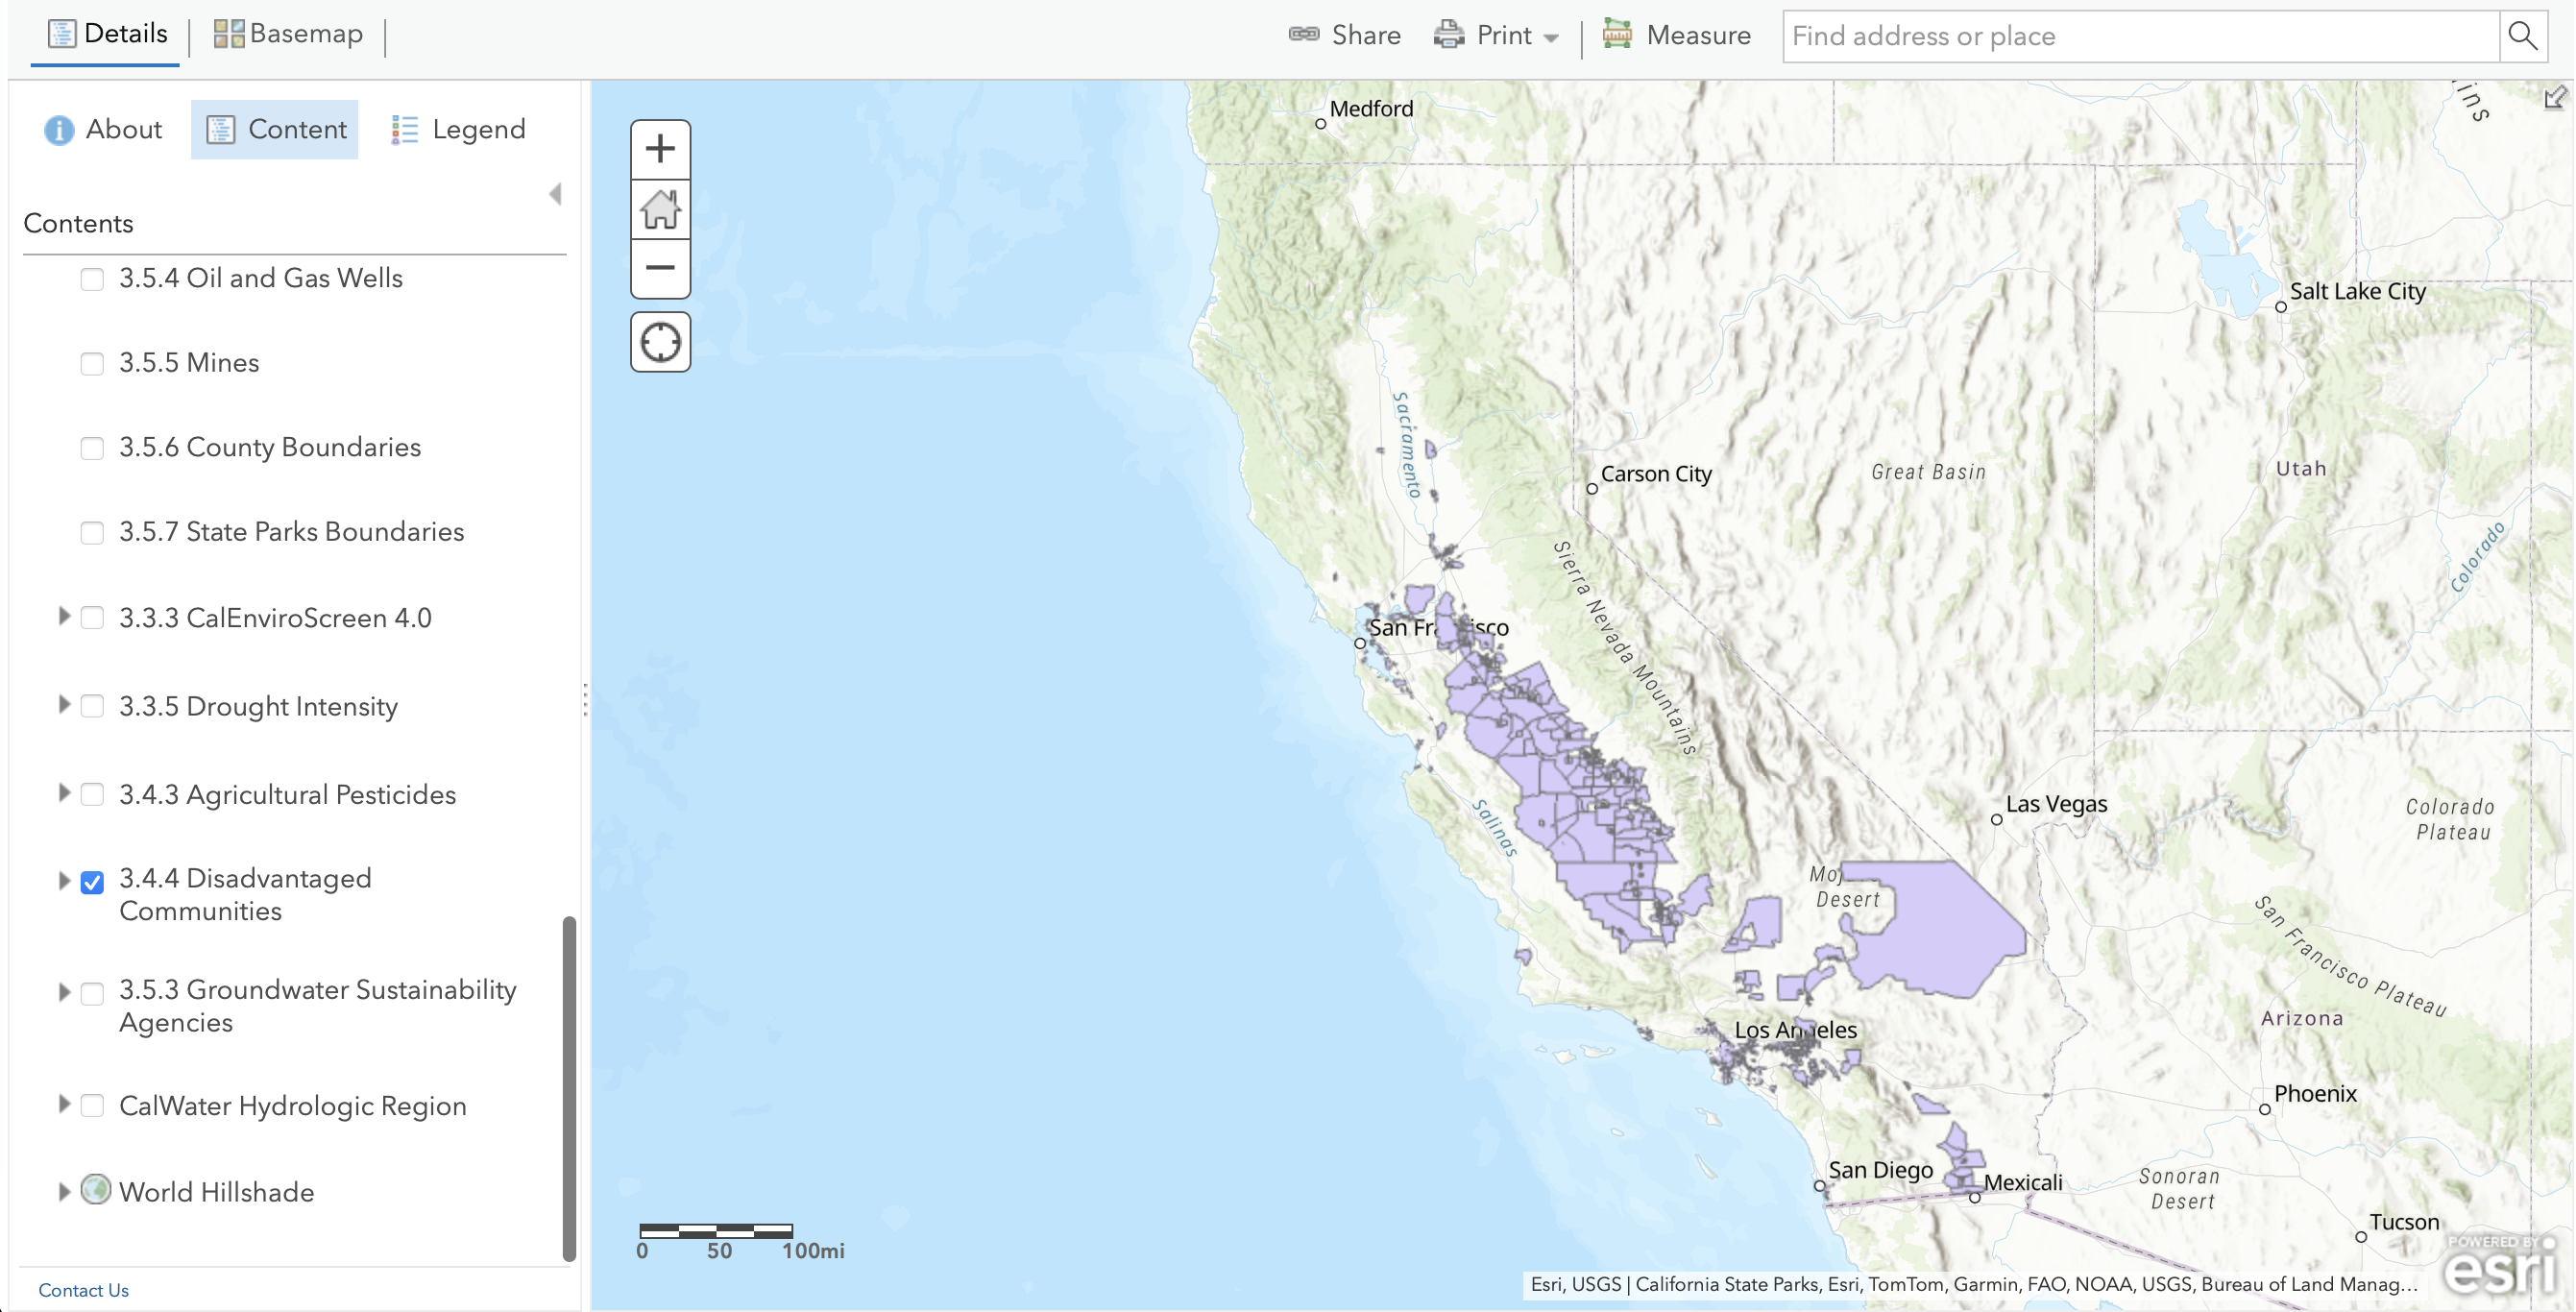
\includegraphics[keepaspectratio]{images/layer-guide_disadvantaged-communities.png}}

Source:
\href{https://oehha.ca.gov/calenviroscreen/report/calenviroscreen-40}{California
Office of Environmental Health Hazard Assessment (OEHHA)}

Data Update Frequency: As needed

Contact:
\href{https://oehha.ca.gov/calenviroscreen/contact-calenviroscreen}{CalEnviroScreen}

\section{Pollution Indicators}\label{pollution-indicators}

\subsection{Agricultural Pesticides}\label{agricultural-pesticides}

This indicator represents the reported use of 132 hazardous and volatile
pesticides in 2017-2019. Only pesticides used on agricultural
commodities are included in the indicator. The data is averaged over the
census tract area, and some application may be adjacent to (instead of
within) the census tract.

\pandocbounded{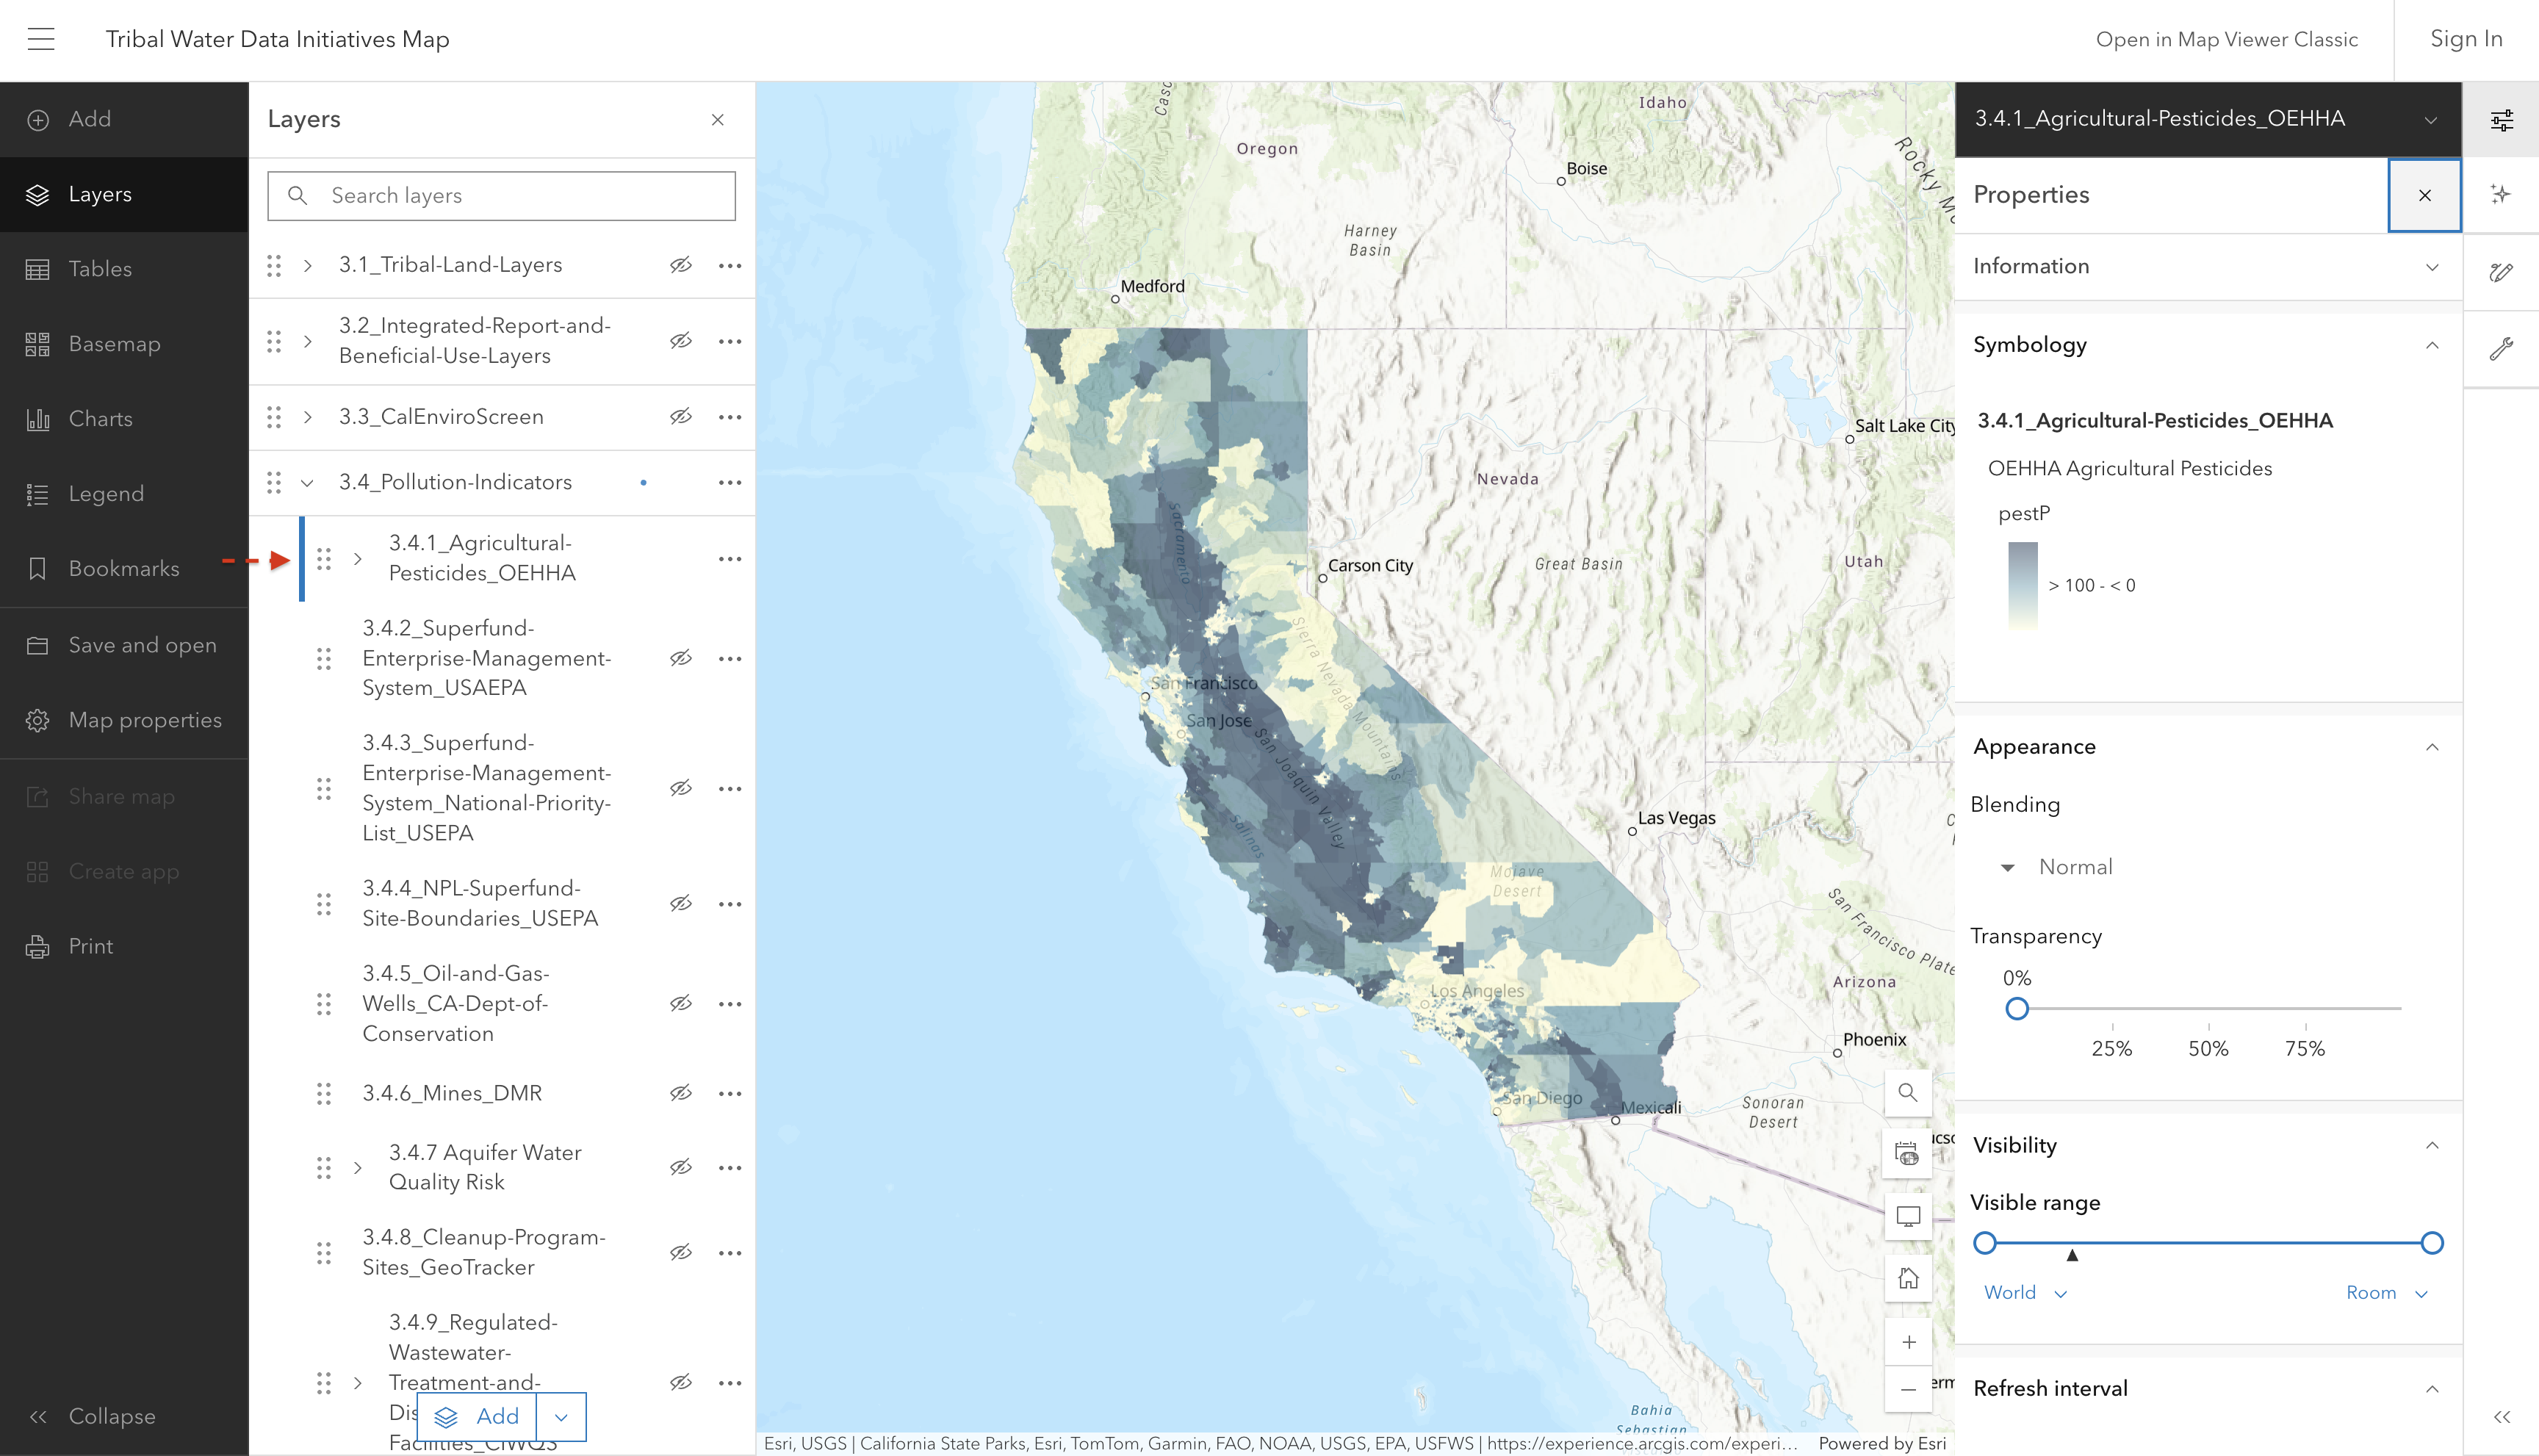
\includegraphics[keepaspectratio]{images/layer-guide_agricultural-pesticides.png}}

Source:
\href{https://experience.arcgis.com/experience/ed5953d89038431dbf4f22ab9abfe40d/page/Indicators?views=Pesticide-Use\#data_s=id\%3AdataSource_40-17c3dec6ede-layer-2\%3A2935}{California
Office of Environmental Health Hazard Assessment (OEHHA)}

Data Update Frequency: As needed

Contact:
\href{https://oehha.ca.gov/calenviroscreen/contact-calenviroscreen}{CalEnviroScreen}

\subsection{Superfund Sites}\label{superfund-sites}

This layer shows Superfund Site locations and data on the inventory of
active and archived hazardous waste sites evaluated by the EPA's
Superfund program.

\pandocbounded{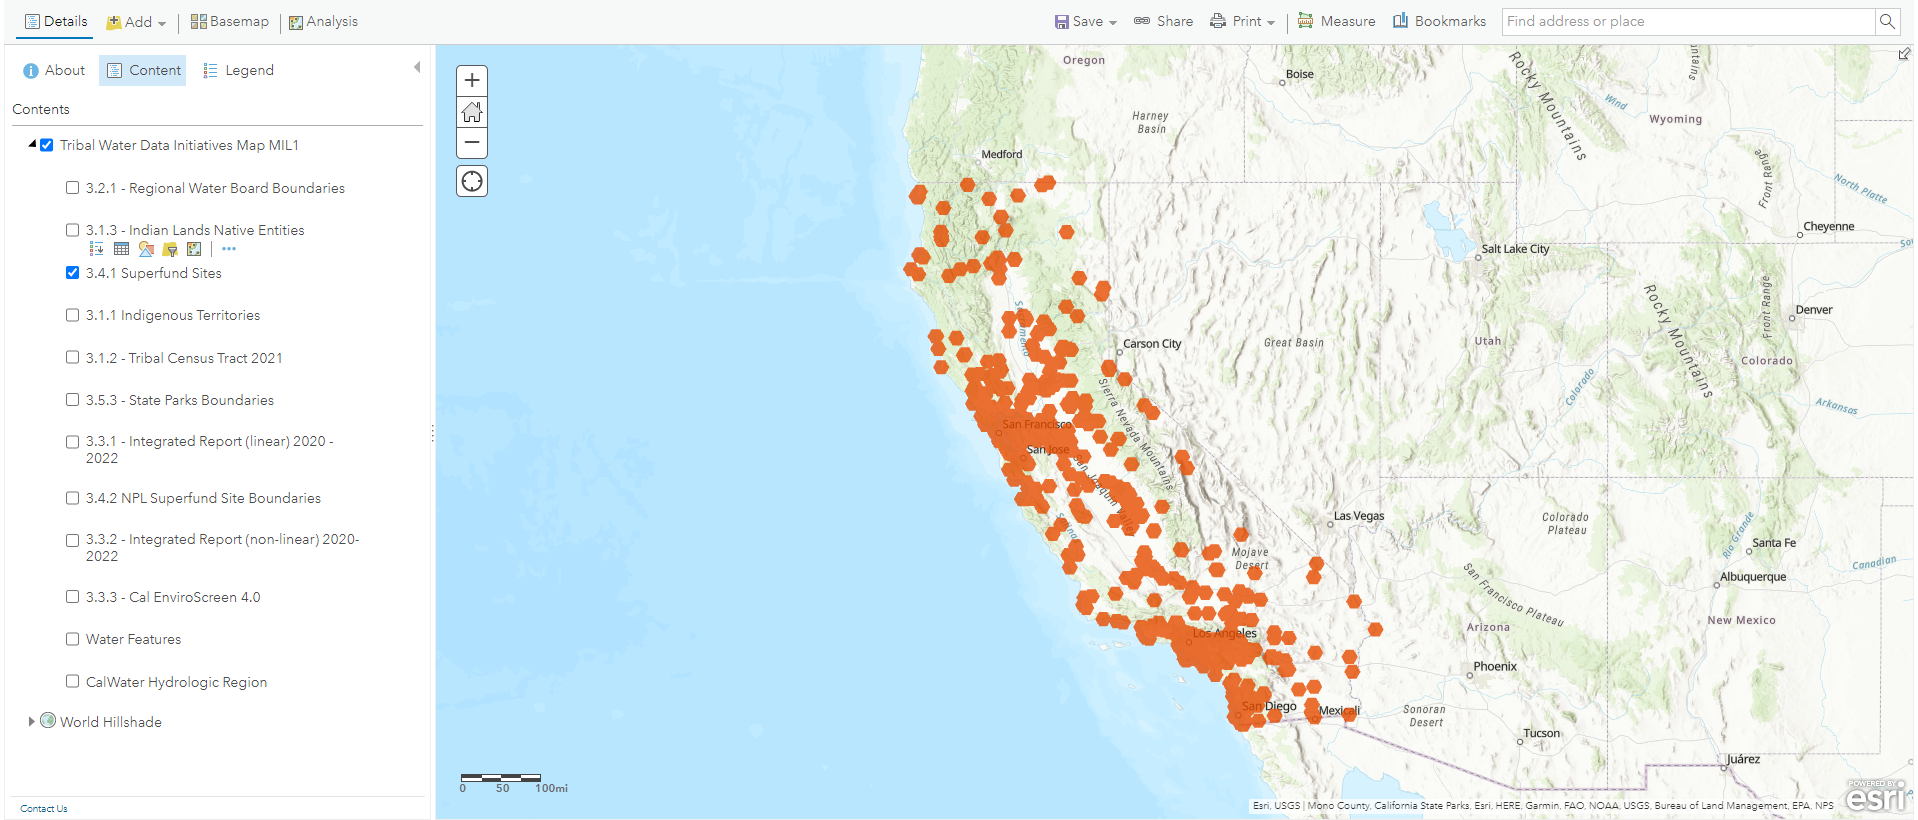
\includegraphics[keepaspectratio]{images/layer-guide_superfund-sites.png}}

This data provides location and attribute information on Facilities
regulated under the Superfund Enterprise Management System (SEMS). It
contains sites that are either proposed to be, or are on, the National
Priorities List (NPL) as well as sites that are in the screening and
assessment phase for possible inclusion on the NPL.

Source:
\href{https://catalog.data.gov/dataset/epa-facility-registry-service-frs-sems8}{U.S.
Environmental Protection Agency (EPA)}

Data Update Frequency: As needed

Contact:
\href{https://usepa.servicenowservices.com/ecss?id=ecss_csm_get_help_1&sys_id=d696a9f51ba9581013bdb913cc4bcbbe}{U.S
Environmental Protection Agency (EPA)}

\subsection{NPL Superfund Site
Boundaries}\label{npl-superfund-site-boundaries}

This layer shows entire Superfund Site boundaries.

\pandocbounded{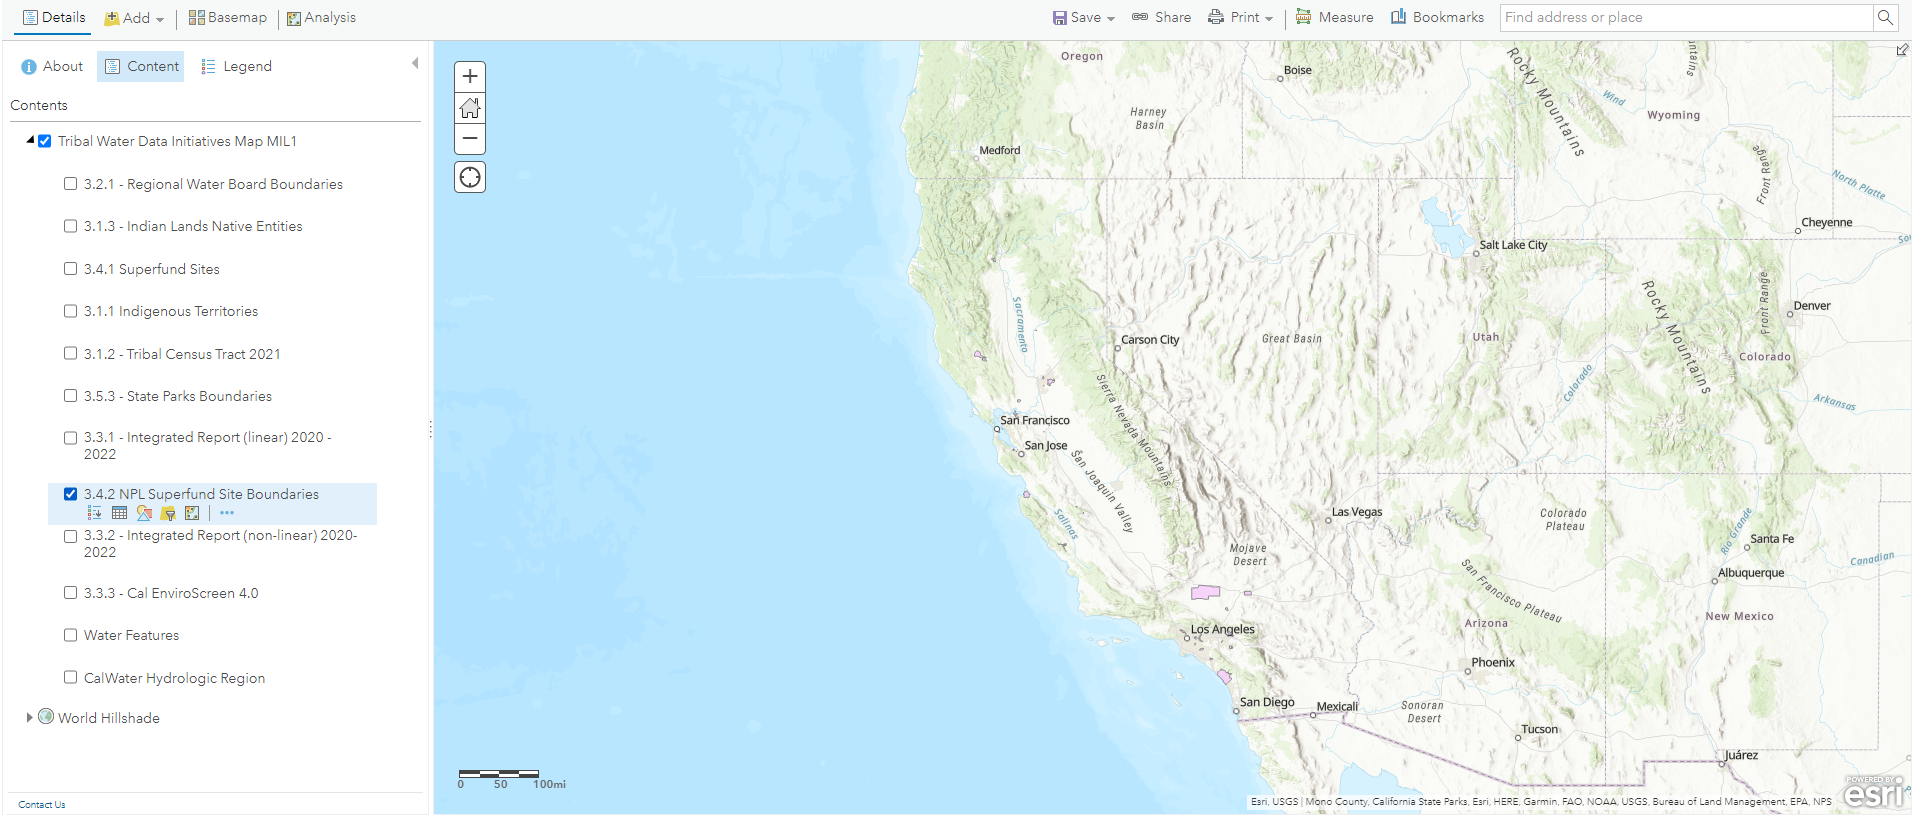
\includegraphics[keepaspectratio]{images/layer-guide_npl-superfund-boundaries.png}}

U.S. EPA Superfund Site boundaries are polygons representing the
footprint of a whole site, defined for purposes of this effort as the
sum of all of the Operable Units and the current understanding of the
full extent of contamination.

Source:
\href{https://catalog.data.gov/dataset/npl-superfund-site-boundaries-epa10}{U.S.
Environmental Protection Agency (EPA)}

Data Update Frequency: Monthly

Last updated: May 25th, 2025

Contact:
\href{https://usepa.servicenowservices.com/ecss?id=ecss_csm_get_help_1&sys_id=d696a9f51ba9581013bdb913cc4bcbbe}{U.S
Environmental Protection Agency (EPA)}

\subsection{Oil and Gas Wells}\label{oil-and-gas-wells}

This layer shows oil and gas well locations (and their associated
records) across California.

\pandocbounded{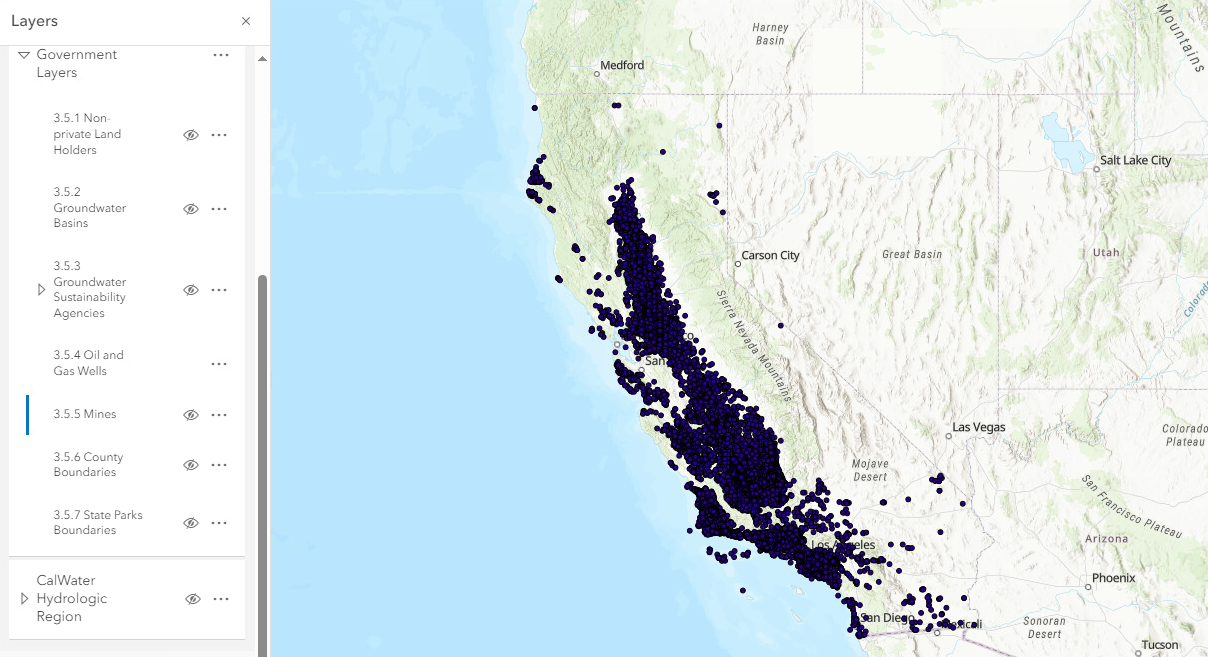
\includegraphics[keepaspectratio]{images/layer-guide-oil-gas-wells.png}}

Source:
\href{https://www.conservation.ca.gov/calgem/Pages/WellFinder.aspx}{WellFinder},
published by the California Department of Conservation and Geologic
Energy Management Division

Data Update Frequency: As needed

\subsection{Mines}\label{mines}

This layer shows all mines in California.

\pandocbounded{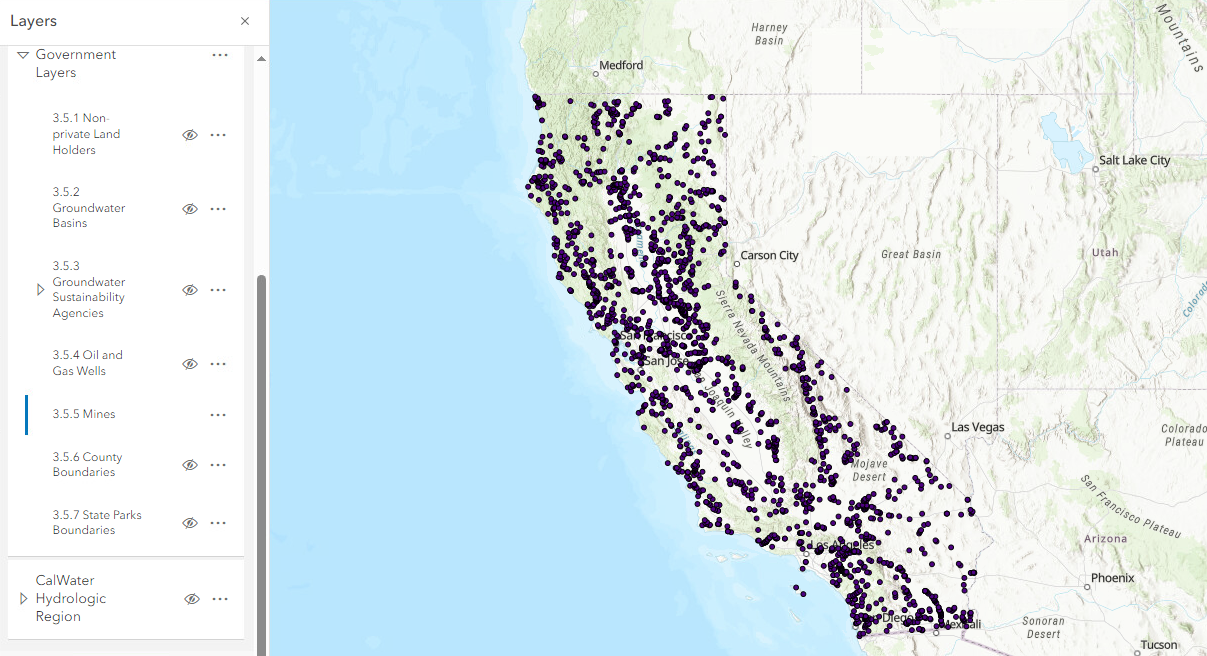
\includegraphics[keepaspectratio]{images/layer-guide-mines.png}}

This data is published with the intent to aid mine reclamation and is
gathered via annual reports under Public Resources Code section 2207.

Source: California Department of Conservation Division of Mine
Reclamation

Data Update Frequency: As needed

\subsection{Aquifer Water Quality
Risk}\label{aquifer-water-quality-risk}

\subsubsection{State Small Water
Systems}\label{state-small-water-systems}

\pandocbounded{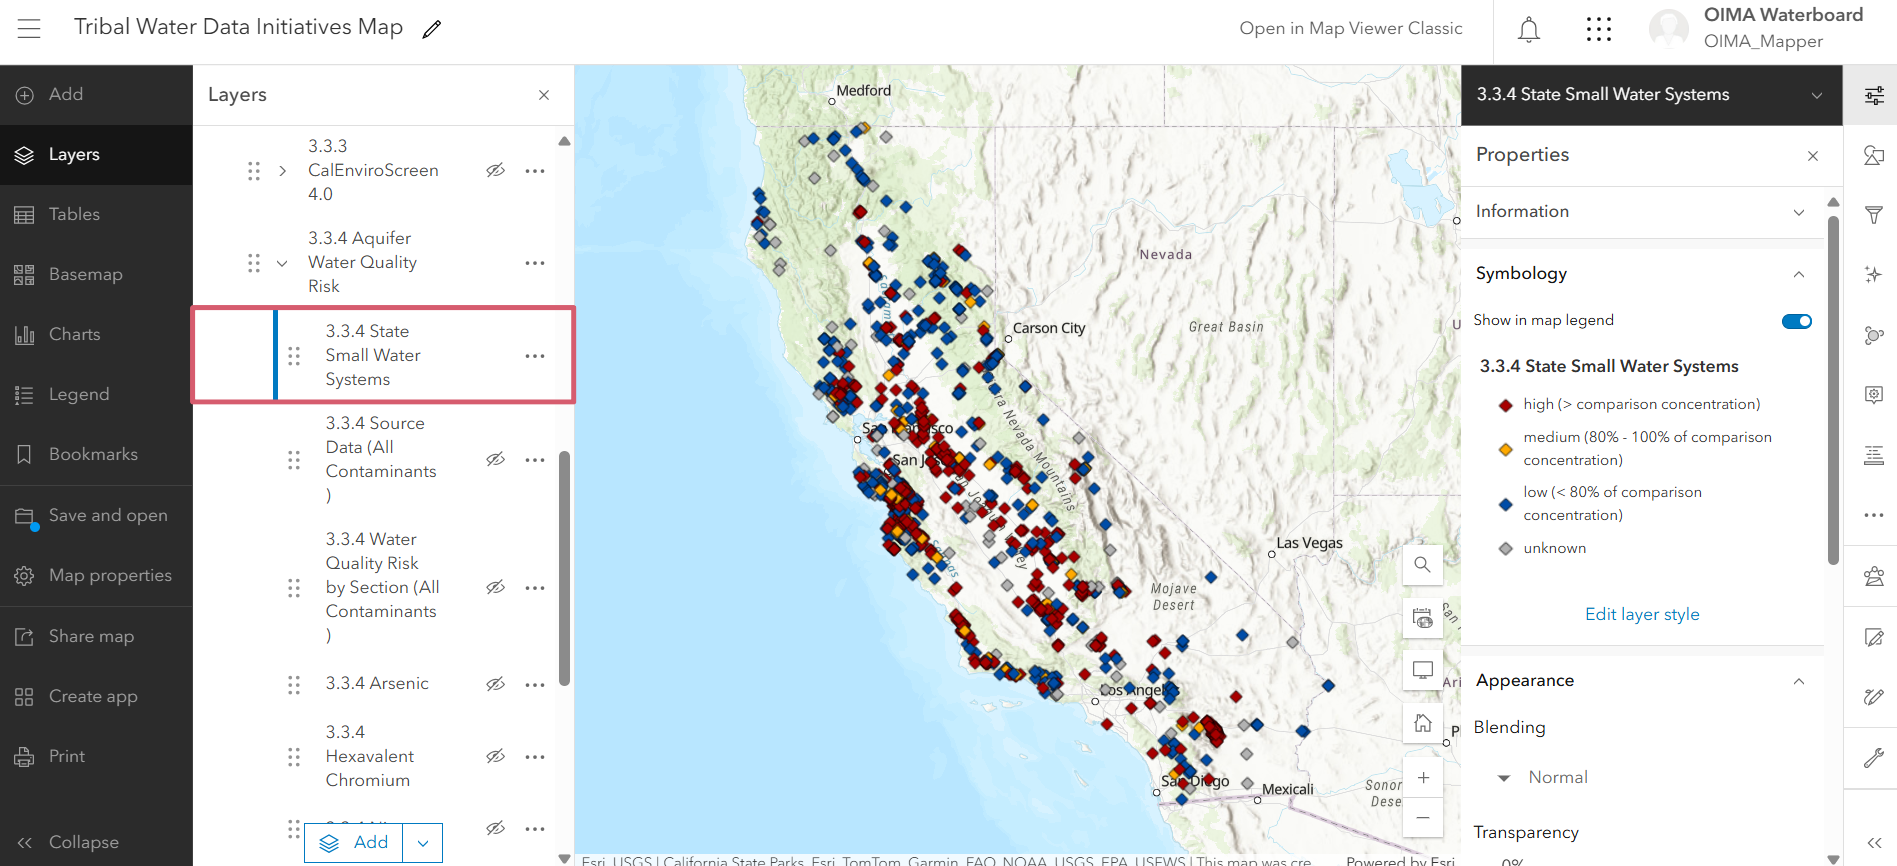
\includegraphics[keepaspectratio]{images/layer-guide_small-water-systems.png}}

\subsubsection{Source Data (All
Contaminants)}\label{source-data-all-contaminants}

\pandocbounded{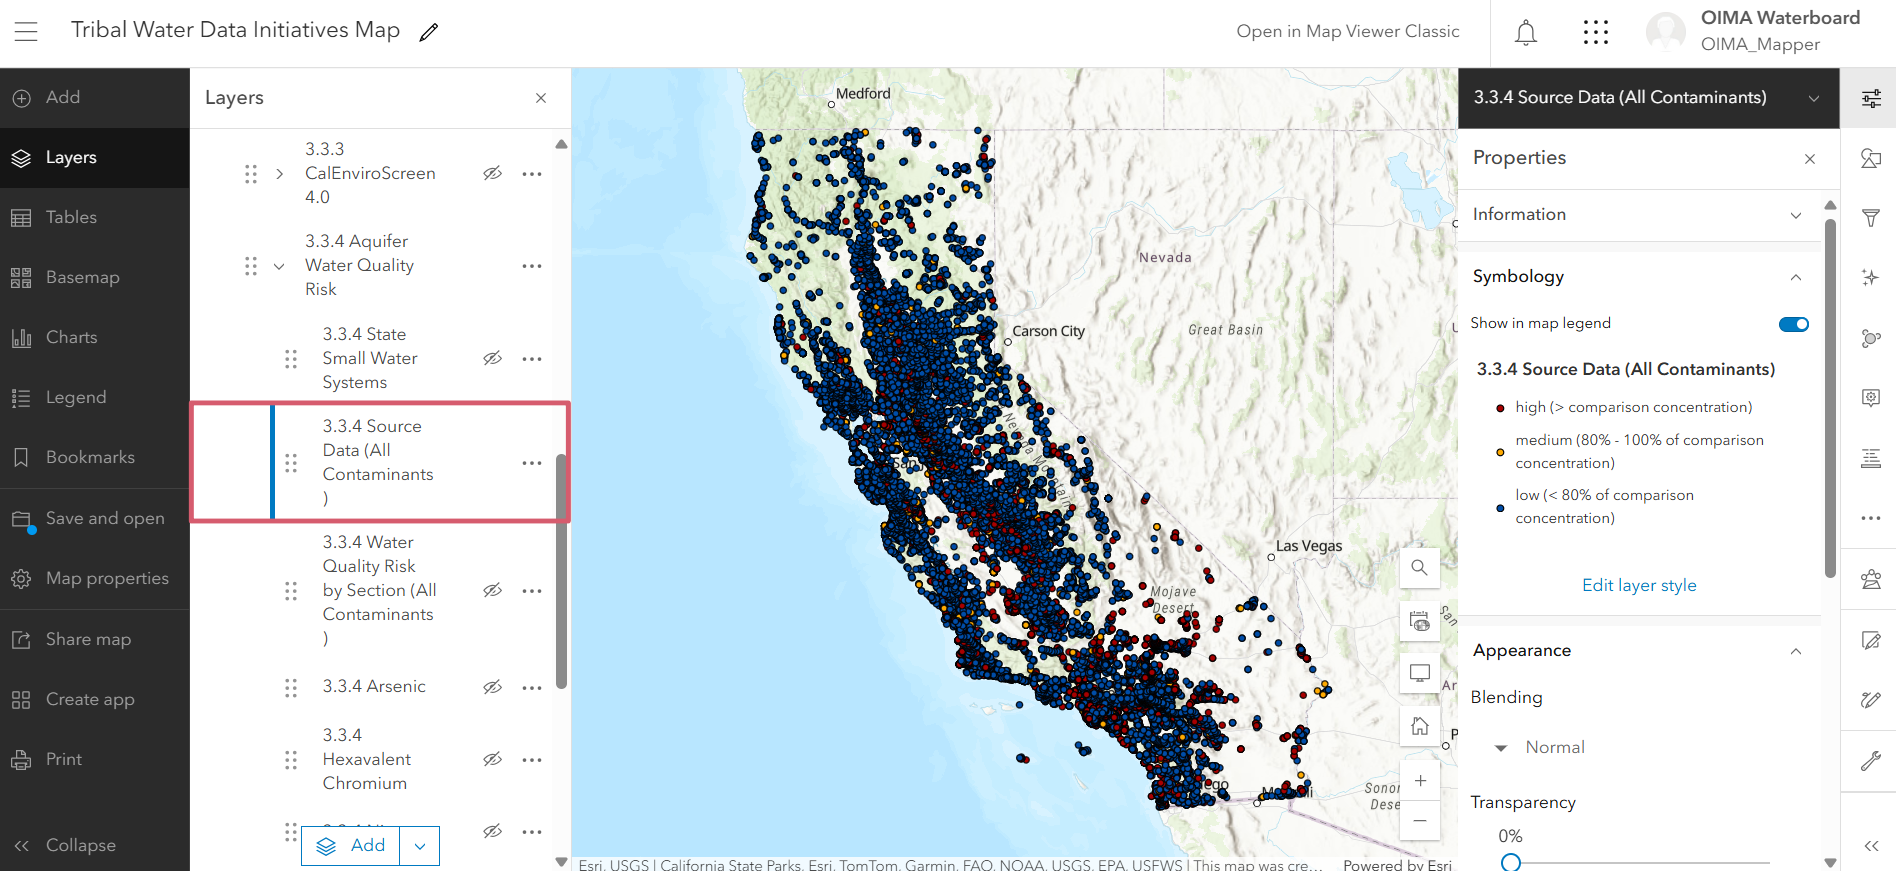
\includegraphics[keepaspectratio]{images/layer-guide_source-contaminants.png}}

\subsubsection{Water Quality Risk by Section (All
Contaminants)}\label{water-quality-risk-by-section-all-contaminants}

This layer shows estimated water quality risk for domestic wells and
state small water systems for a variety of contaminants.

\pandocbounded{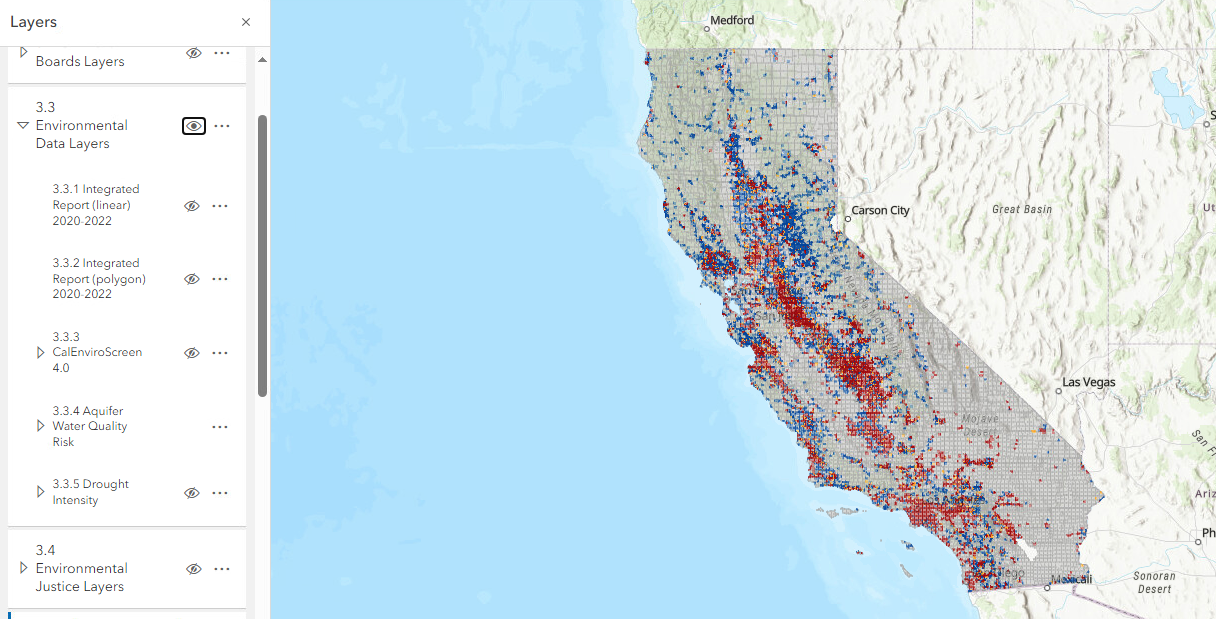
\includegraphics[keepaspectratio]{images/layer-guide-aquifer-water-quality.png}}

This layer was developed for use by the State Water Boards SAFER Program
to help prioritize areas where domestic wells and state small water
systems may be accessing groundwater that does not meet primary drinking
water standards.

Source: \href{https://www.waterboards.ca.gov/gama/}{Groundwater Ambient
Monitoring and Assessment (GAMA) Program}

Data Update Frequency: As needed

Contact: \href{https://www.waterboards.ca.gov/safer/}{SAFER Program}

\subsubsection{Arsenic}\label{arsenic}

\subsubsection{Hexavalent Chromium}\label{hexavalent-chromium}

\subsubsection{Nitrate}\label{nitrate}

\subsubsection{Tricholoropropane}\label{tricholoropropane}

\subsubsection{Uranium}\label{uranium}

\subsection{Cleanup Program Sites}\label{cleanup-program-sites}

\begin{tcolorbox}[enhanced jigsaw, breakable, title=\textcolor{quarto-callout-note-color}{\faInfo}\hspace{0.5em}{Note}, coltitle=black, colframe=quarto-callout-note-color-frame, opacitybacktitle=0.6, colback=white, opacityback=0, bottomrule=.15mm, colbacktitle=quarto-callout-note-color!10!white, leftrule=.75mm, bottomtitle=1mm, toptitle=1mm, toprule=.15mm, left=2mm, titlerule=0mm, arc=.35mm, rightrule=.15mm]

The Cleanup Program Sites have 36 different classifications. For ease of
viewing on this map, we have combined similar classifications into
groups. You can find the specific classification if you click on the
individual point of interest, or you can refer here for the full list.

\end{tcolorbox}

Source:
\href{https://geotracker.waterboards.ca.gov/datadownload}{GeoTracker}

Data Update Frequency: Daily

Last Updated: downloaded 2025/05/21

\subsection{Regulated Wastewater Treatment \& Discharge
Facilities}\label{regulated-wastewater-treatment-discharge-facilities}

Layer showing National Pollutant Discharge Elimination System (NPDES)
and Waste Discharge Requirements (WDR) facilities regulated by State
Water Board programs, as reflected in the California Integrated Water
Quality System (CIWQS) project.

\pandocbounded{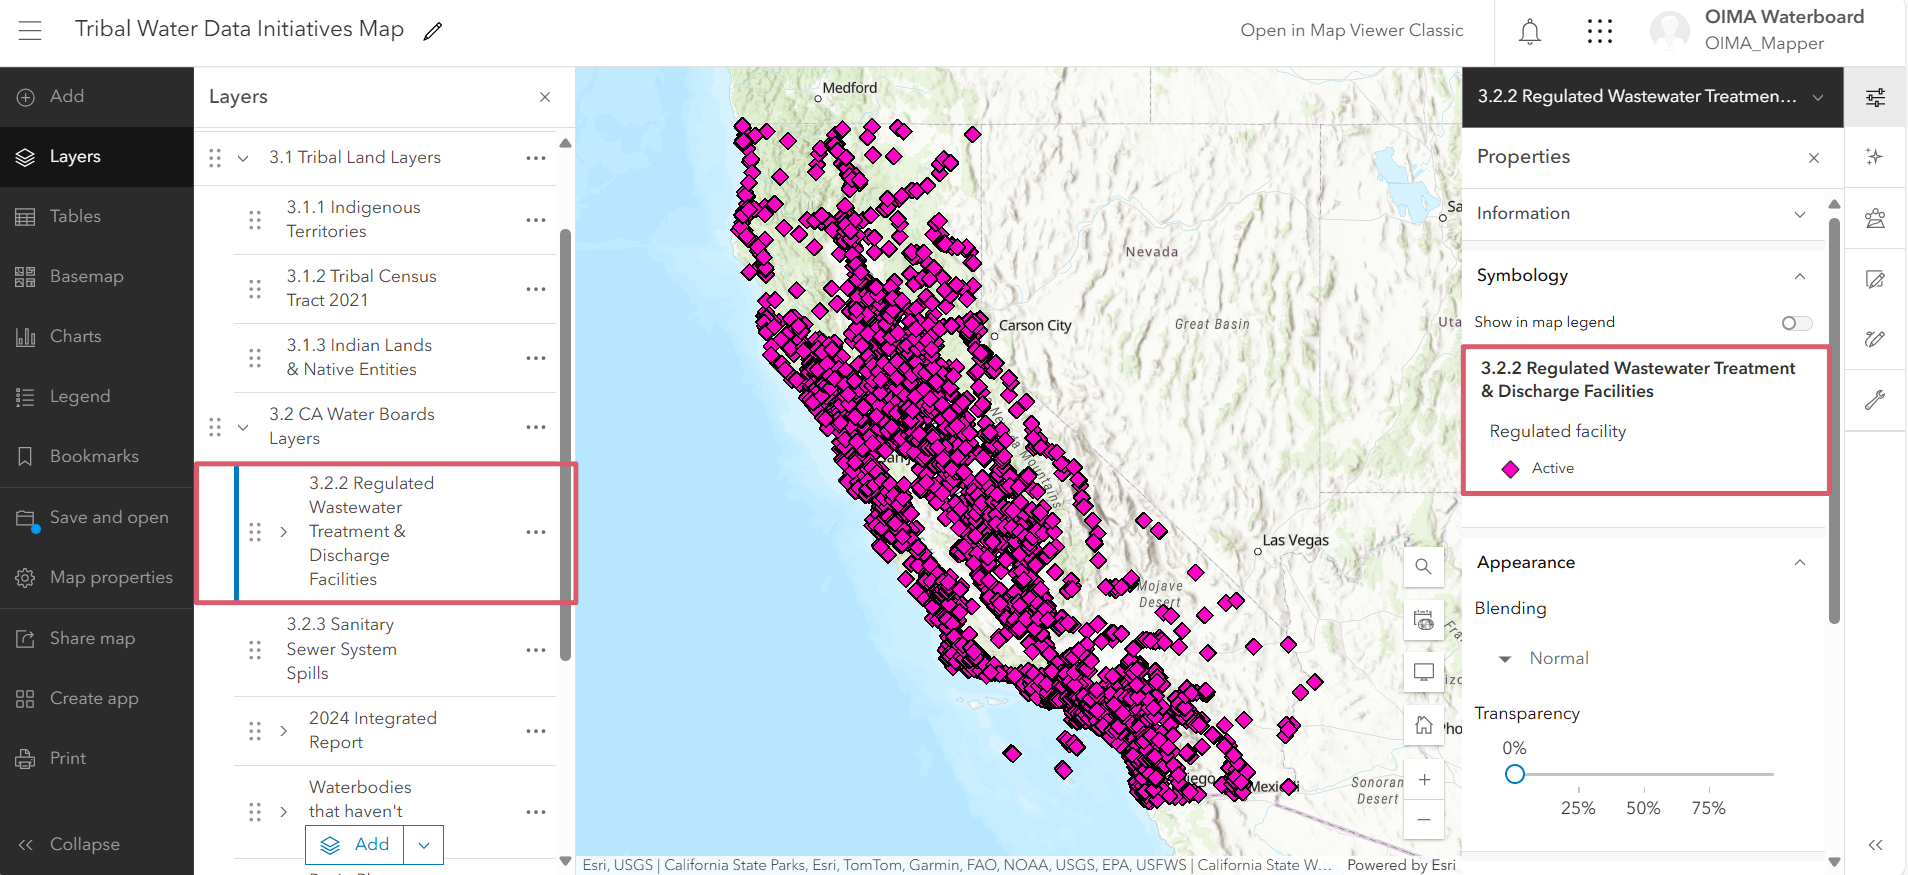
\includegraphics[keepaspectratio]{images/layer-guide_regulated_facilities.png}}

These facilities are mandated to hold active permits to discharge into
or alter the surface or ground water. More information about these
permits can be found in the CIWQS database.

Source:
\href{https://www.waterboards.ca.gov/ciwqs/publicreports.html}{California
Integrated Water Quality System (CIWQS)}

Data Update Frequency: Nightly

\subsection{Sanitary Sewer System
Spills}\label{sanitary-sewer-system-spills}

Layer showing locations with XXXXXXXX

\pandocbounded{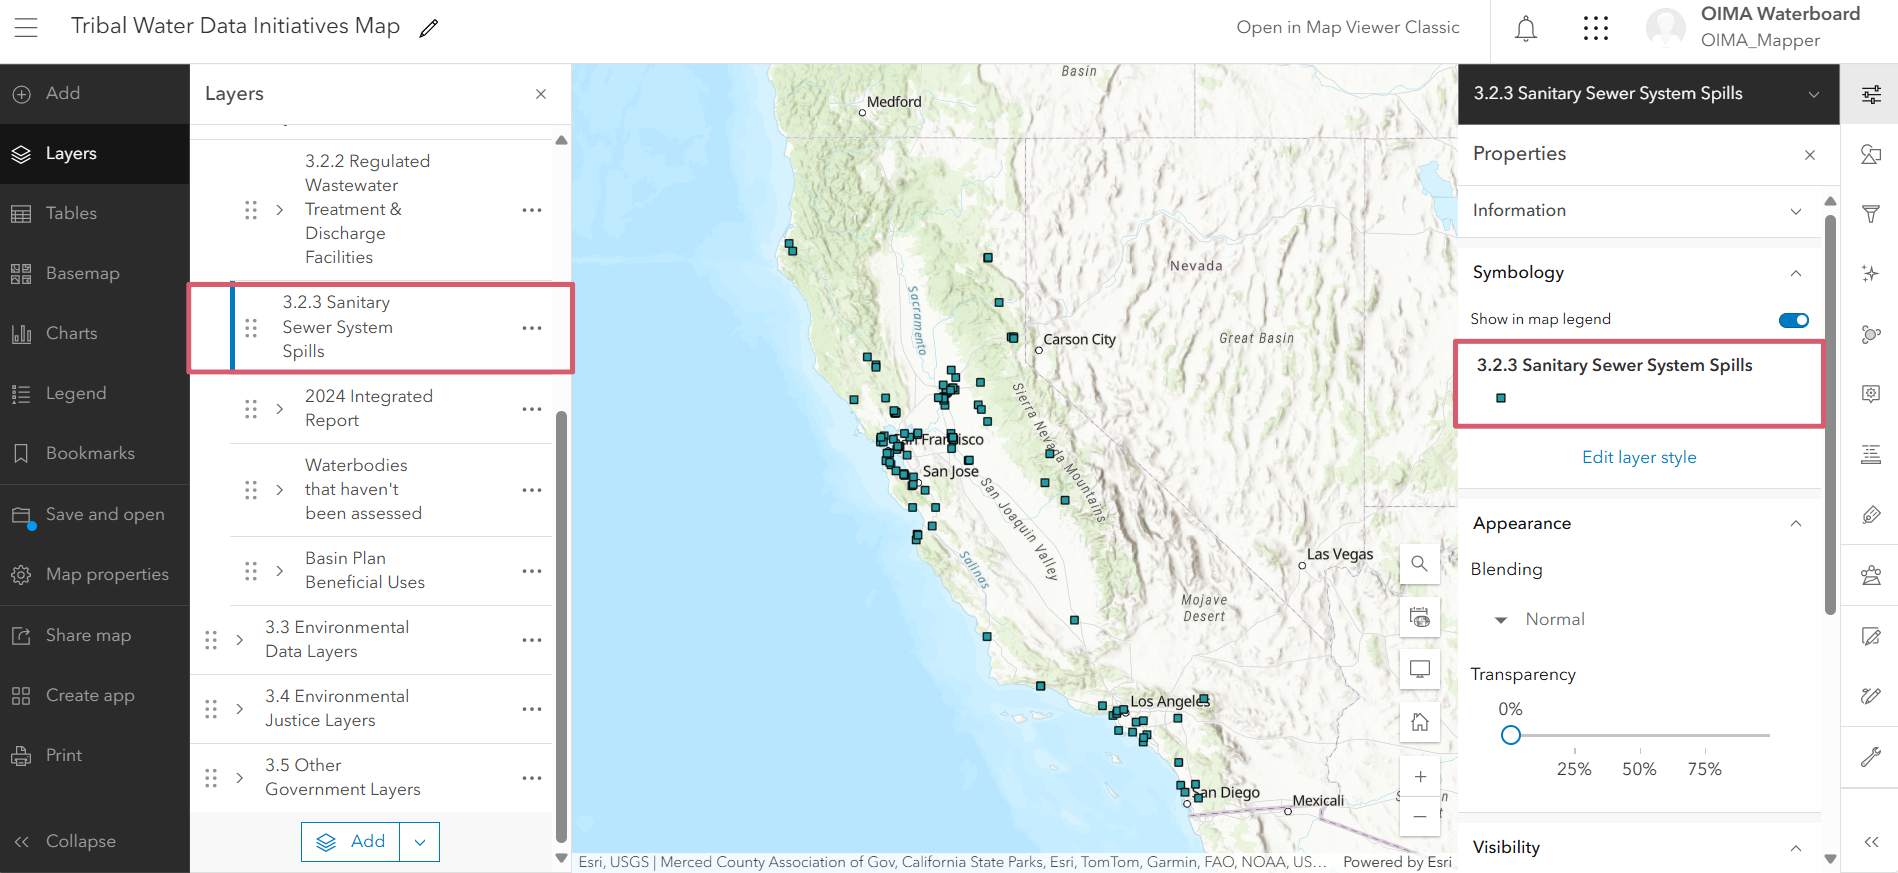
\includegraphics[keepaspectratio]{images/layer-guide_sanitary-sewer-spills.png}}

Source:

Data Update Frequency:

\section{Water Quality}\label{water-quality}

\emph{New layers coming soon}

\section{Climate Change Indicators}\label{climate-change-indicators}

\subsection{Drought Intensity}\label{drought-intensity}

Drought Outlook: This layer shows regions in California impacted by
drought.

\pandocbounded{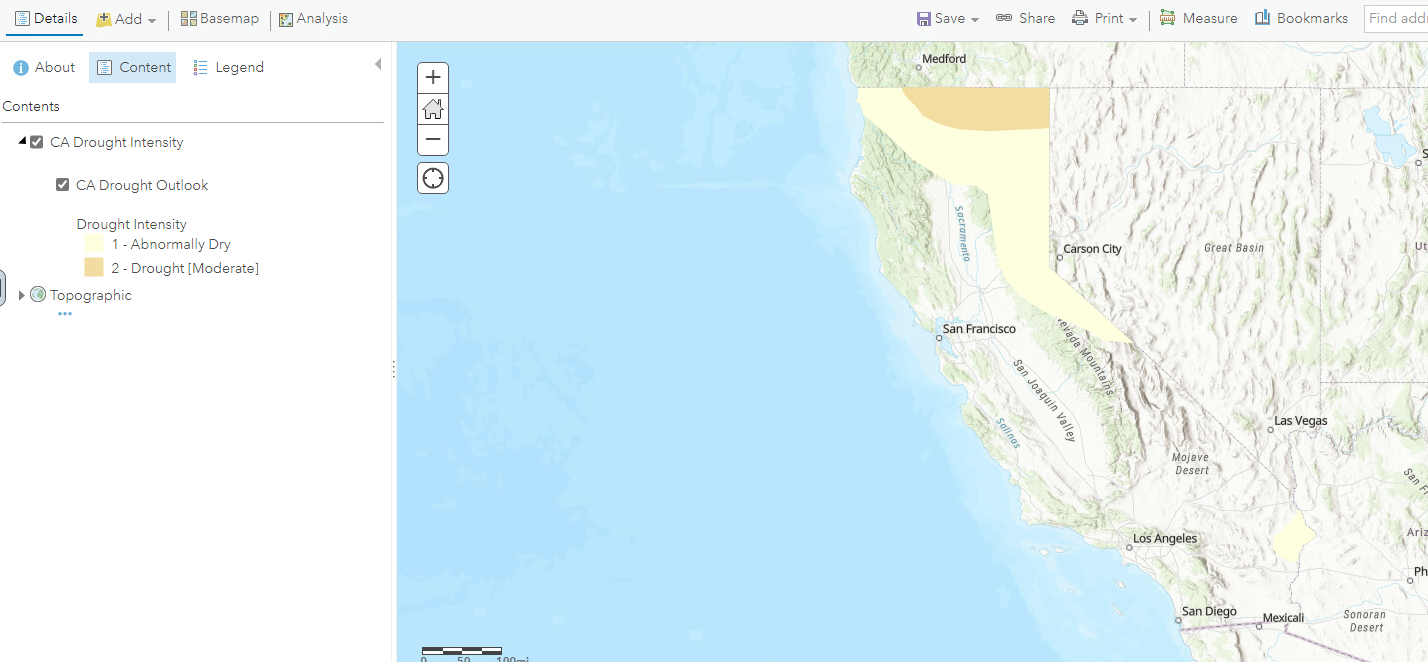
\includegraphics[keepaspectratio]{images/layer-guide_drought_intensity_layer.png}}

Drought severity is determined by precipitation deviation, stream flow,
soil moisture content, subjective observation, and reported impact.

Source: \href{https://droughtmonitor.unl.edu/}{U.S. Drought Monitor}

Data Update Frequency: Weekly, on Thursdays

Contact: \href{https://drought.unl.edu/}{National Drought Mitigation
Center (NDMC)}

\section{Hydrology}\label{hydrology}

\subsection{Groundwater Basins}\label{groundwater-basins}

This layer shows the boundaries of 515 groundwater basins and subbasins
as defined by the California Department of Water Resources.

\pandocbounded{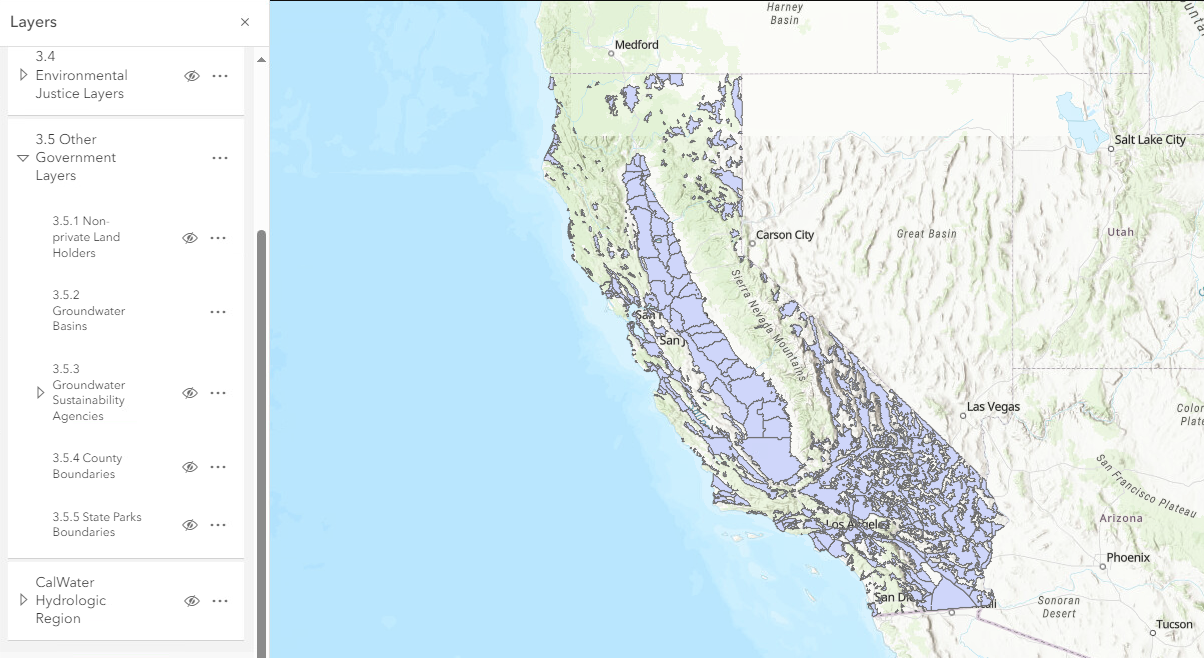
\includegraphics[keepaspectratio]{images/layer-guide-groundwater-basins.png}}

Source:
\href{https://data.ca.gov/dataset/i08-b118-ca-groundwaterbasins/resource/0bb7282a-e0b1-452f-a364-da785911843e}{California
Department of Water Resources}

Data Update Frequency: As needed

\subsection{Hydrography, Water
Boundaries}\label{hydrography-water-boundaries}

The California Interagency Watershed Map is the State of California's
working definition of watershed boundaries. Previous Calwater versions
described California watersheds, beginning with the division of the
State's 101 million acres into ten \textbf{Hydrologic Regions}~(HR).
Each HR is progressively subdivided into six smaller, nested levels: the
\textbf{Hydrologic Unit}~(HU, major rivers),~\textbf{Hydrologic
Area}~(HA, major tributaries),~\textbf{Hydrologic Sub-Area}~(HSA), Super
Planning Watershed (\textbf{SPW}), and Planning Watershed (\textbf{PW}),
with the Planning Watershed as the most detailed level. See
\href{https://gispublic.waterboards.ca.gov/portal/home/item.html?id=6f85ec66bc004820a00de6f5ac8be24d}{metadata}
for more information.

\emph{Screenshot here}

Source:
\href{https://gispublic.waterboards.ca.gov/portal/home/item.html?id=816893ddab33434989eda92dbc0e126f}{CalWater
Watersheds - Overview}

Data Update Frequency: As needed

Last Updated: September 7th, 2023

\section{Geopolitical Boundaries}\label{geopolitical-boundaries}

\subsection{Regional Water Board
Boundaries}\label{regional-water-board-boundaries}

Layer showing the boundaries of the nine Regional Water Quality Control
Boards in California.

\pandocbounded{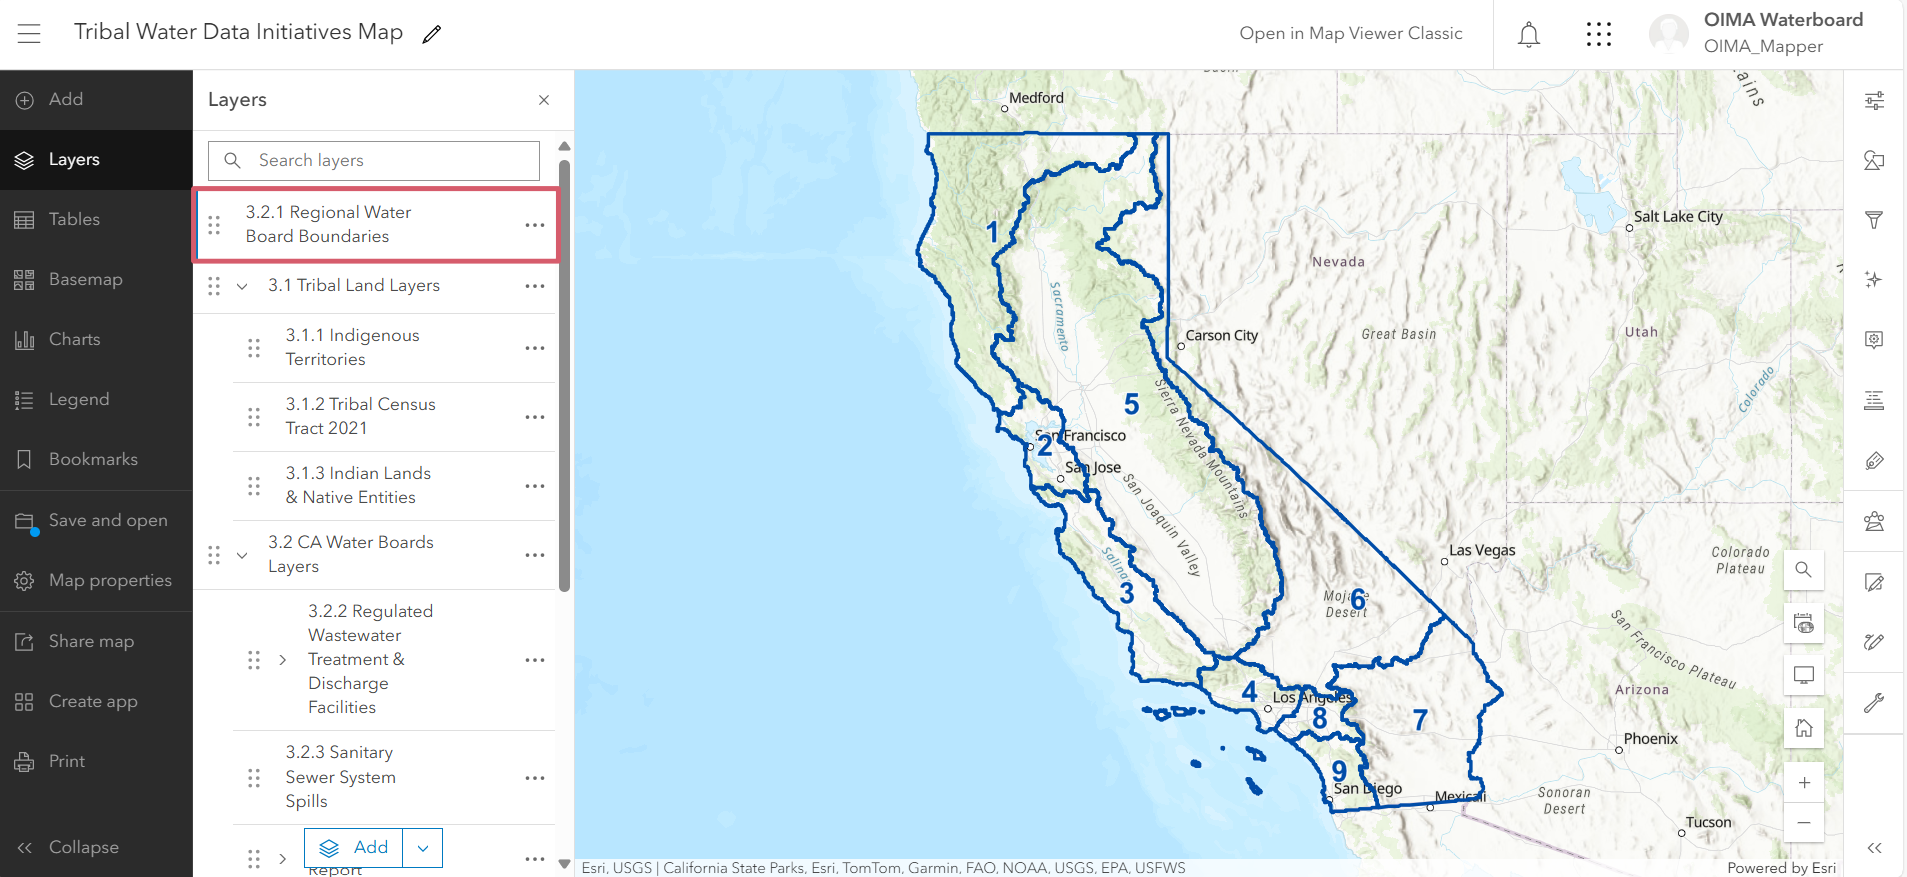
\includegraphics[keepaspectratio]{images/layer-guide_regional-board-boundaries.png}}

Source:
\href{https://gispublic.waterboards.ca.gov/portalserver/rest/services/Tribal_Water_Data_Initiatives_Map_MIL1/MapServer/0}{California
State Water Resources Control Board (SWRCB)}

Data Update Frequency: As needed

\subsection{Census Tracts}\label{census-tracts}

\subsection{County Boundaries}\label{county-boundaries}

This layer shows County boundaries within California.

\pandocbounded{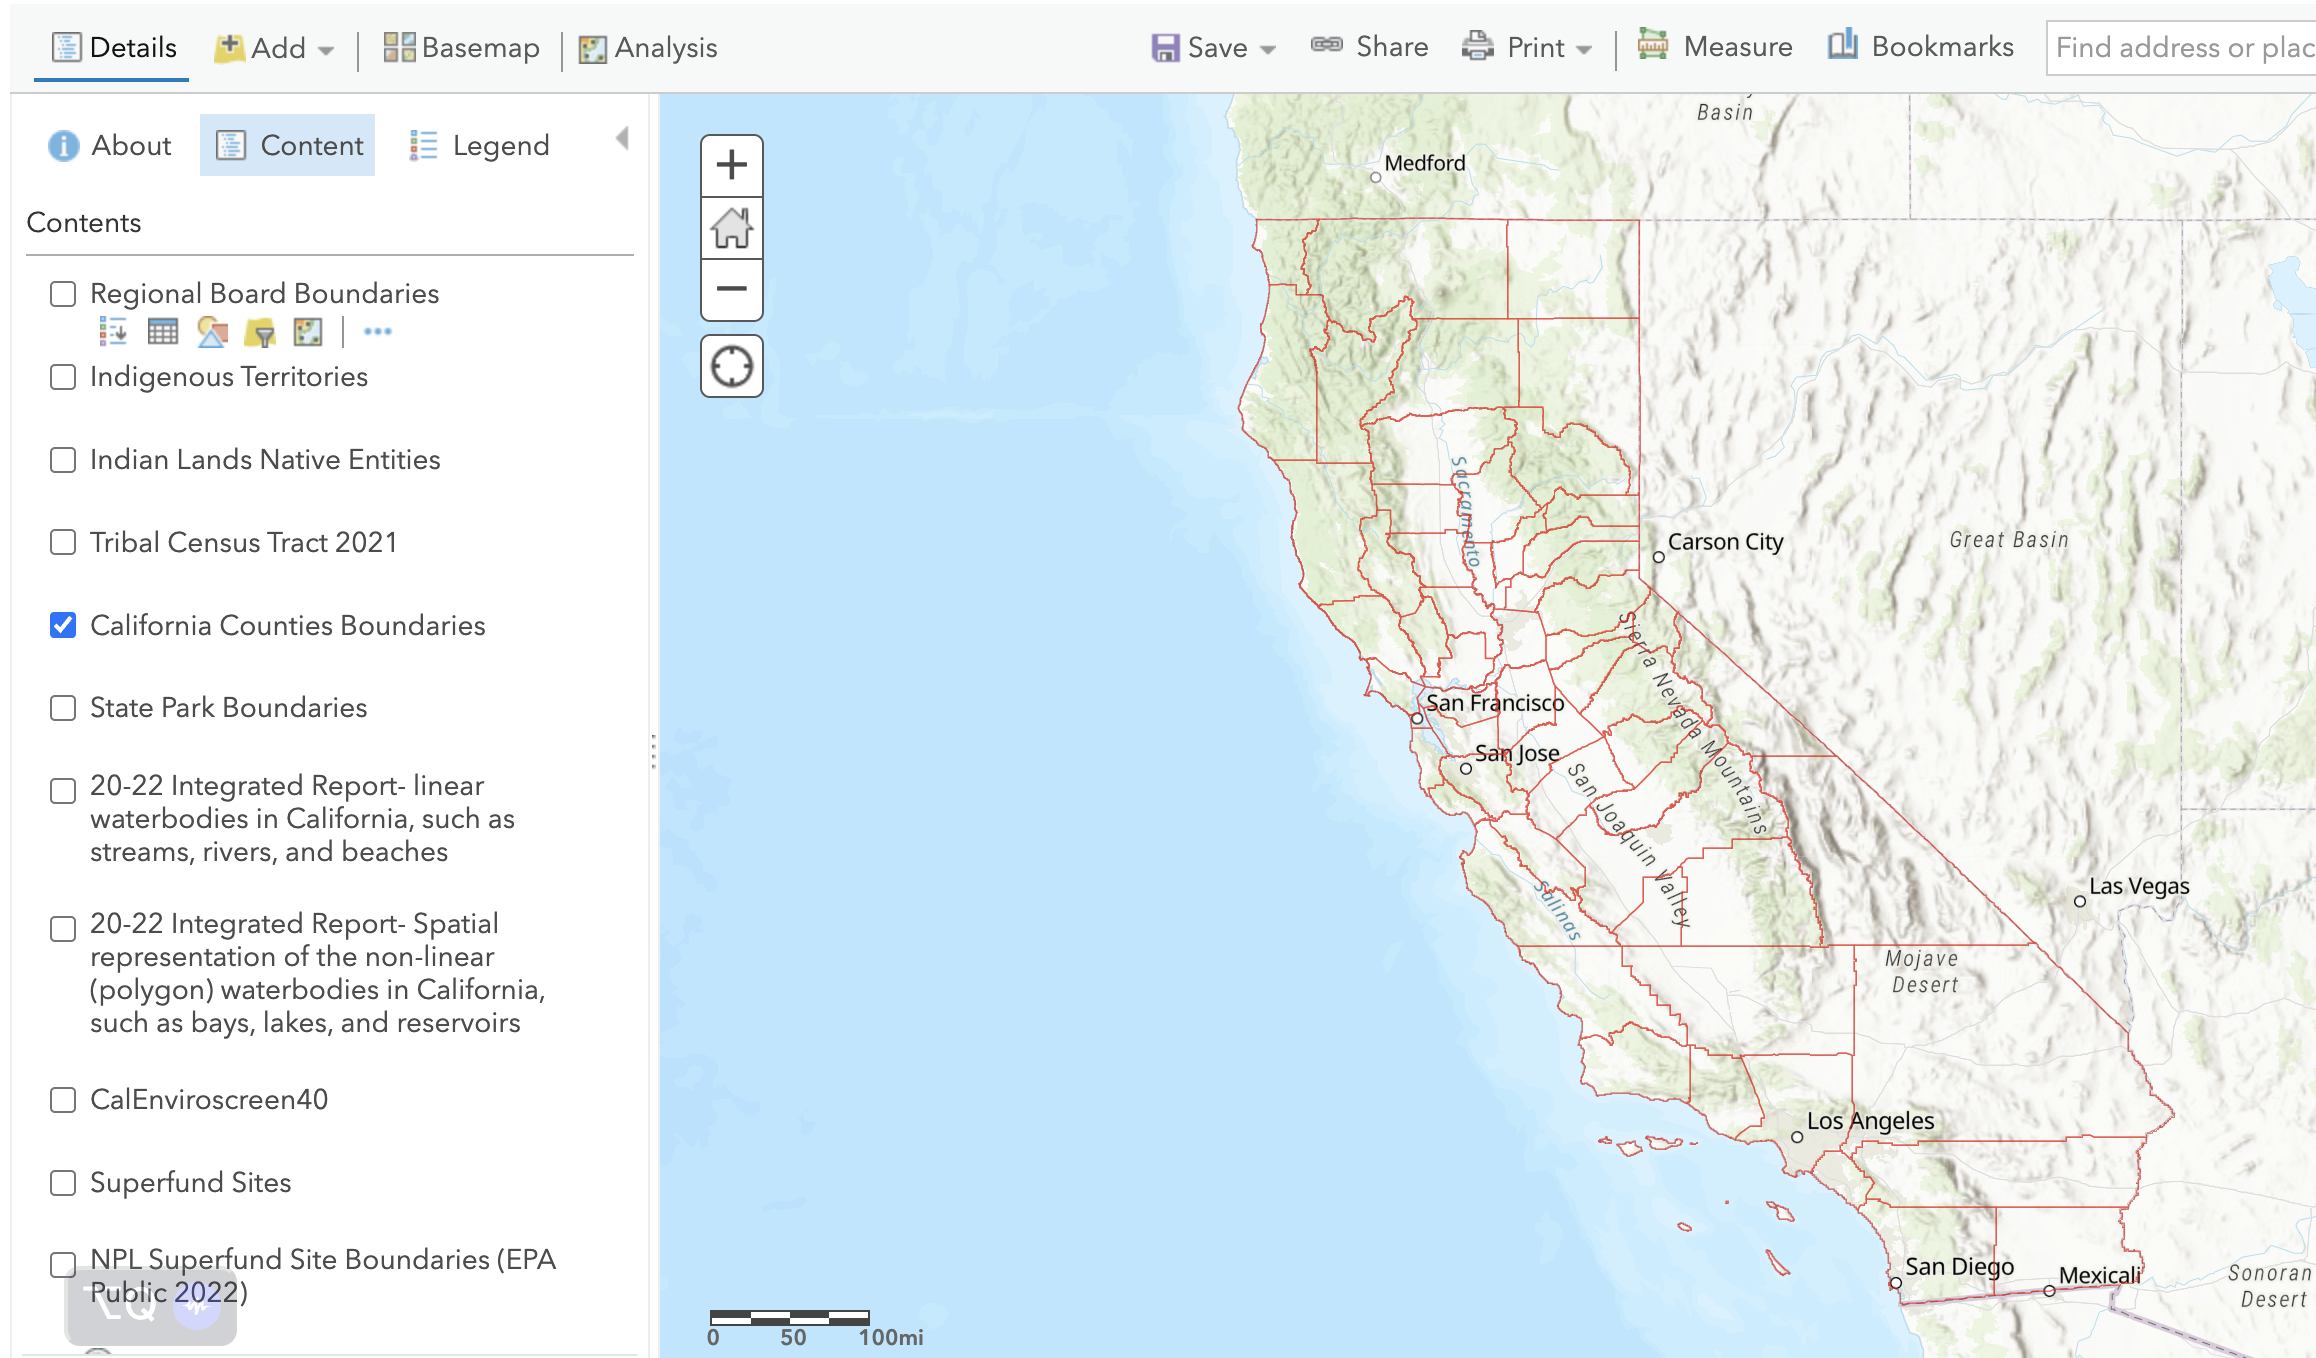
\includegraphics[keepaspectratio]{images/layer-guide_california-counties.png}}

In this dataset, all bays (plus bay islands and constructed features)
are merged into the mainland, and coastal features (such as islands and
constructed features) are not included, with the exception of the
Channel Islands which ARE included.

Source:
\href{https://hub.arcgis.com/datasets/CALFIRE-Forestry::california-counties/about}{California
Dept. of Forestry and Fire Protection (CalFIRE)}

Data Update Frequency: As needed

\subsection{Non-private Land Holders}\label{non-private-land-holders}

This layer shows boundaries for non-private land holders in California.

\pandocbounded{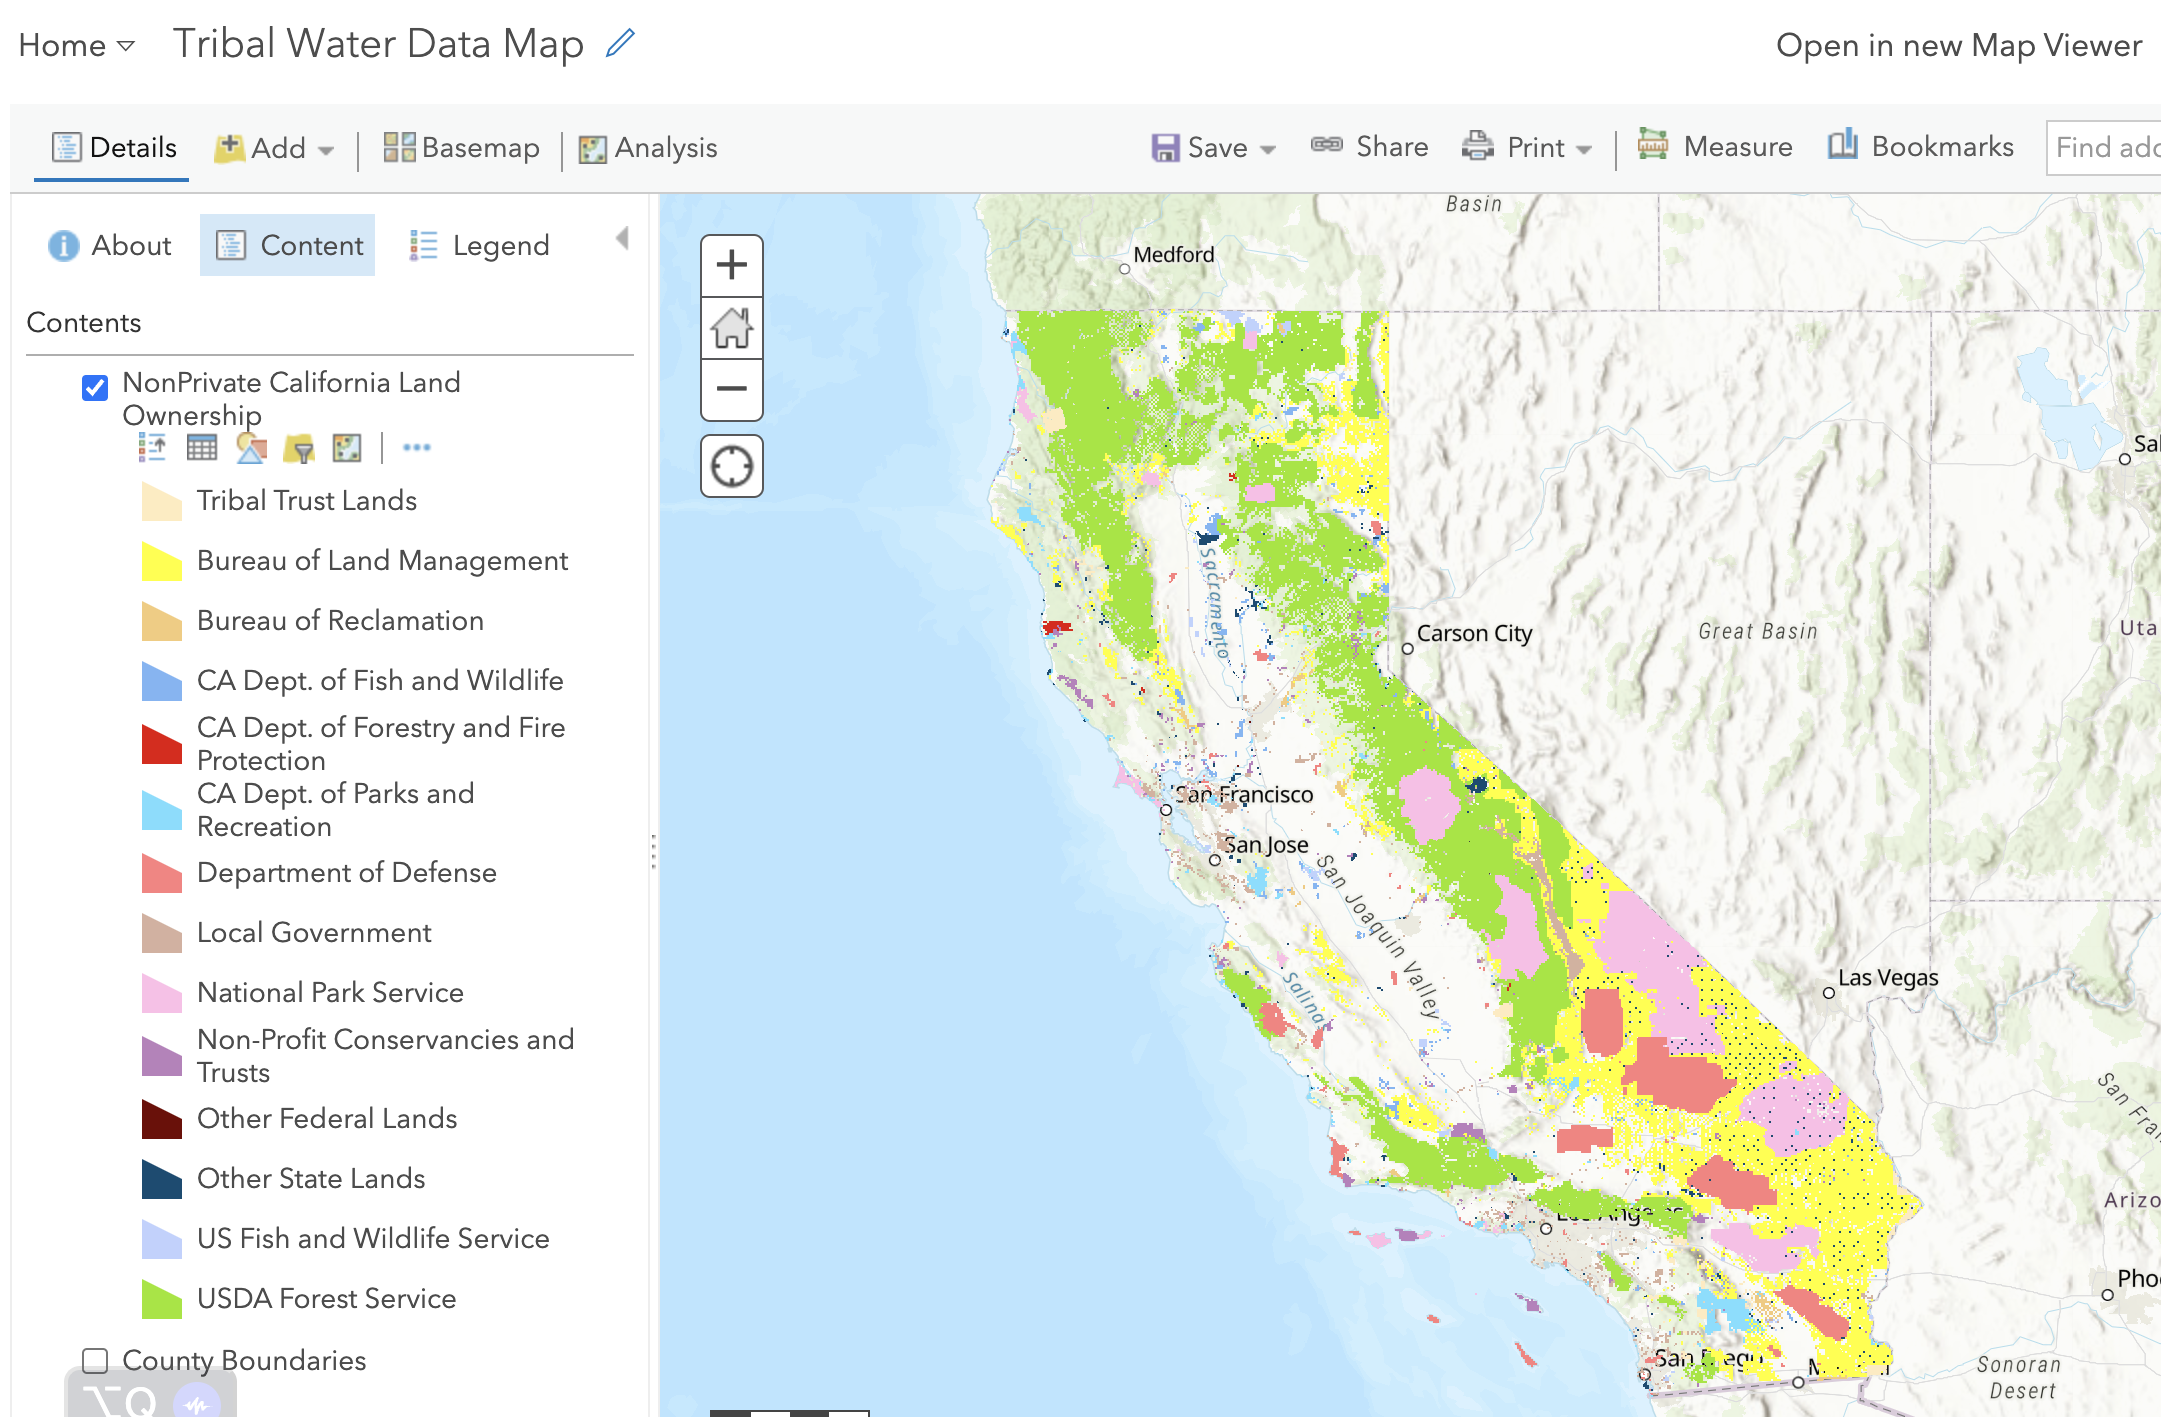
\includegraphics[keepaspectratio]{images/layer-guide_non-private-land-holders.png}}

Source:
\href{https://gis.data.ca.gov/datasets/CALFIRE-Forestry::california-land-ownership/about}{California
Land Ownership \textbar{} California State Geoportal}

Data Update Frequency: As needed

\subsection{California National Parks}\label{california-national-parks}

\subsection{State Park Boundaries}\label{state-park-boundaries}

This layer shows the State Parks in California.

\pandocbounded{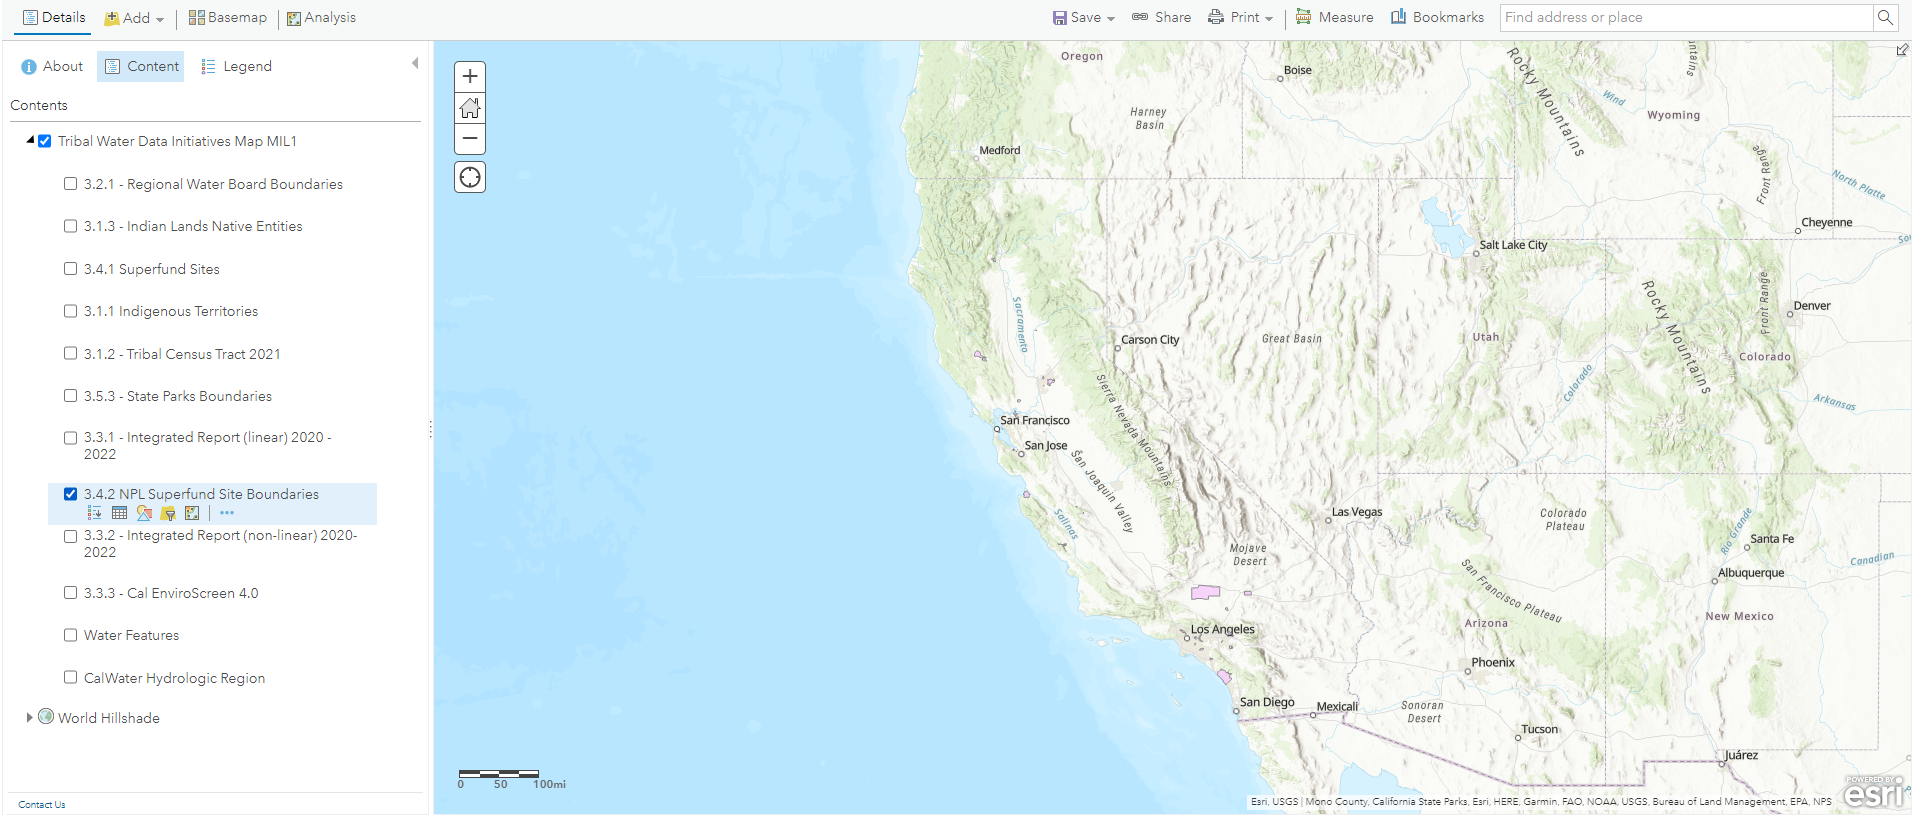
\includegraphics[keepaspectratio]{images/layer-guide_statepark-boundaries-01.png}}

Source: \href{https://www.parks.ca.gov/?page_id=29682}{California Dept.
of Pesticides Regulation (DPR)}

Data Update Frequency: As needed

\subsection{Groundwater Sustainability
Agencies}\label{groundwater-sustainability-agencies}

This layer shows the boundaries of California's Groundwater
Sustainability Agencies as defined on the DWR SGMA Data Viewer.

\pandocbounded{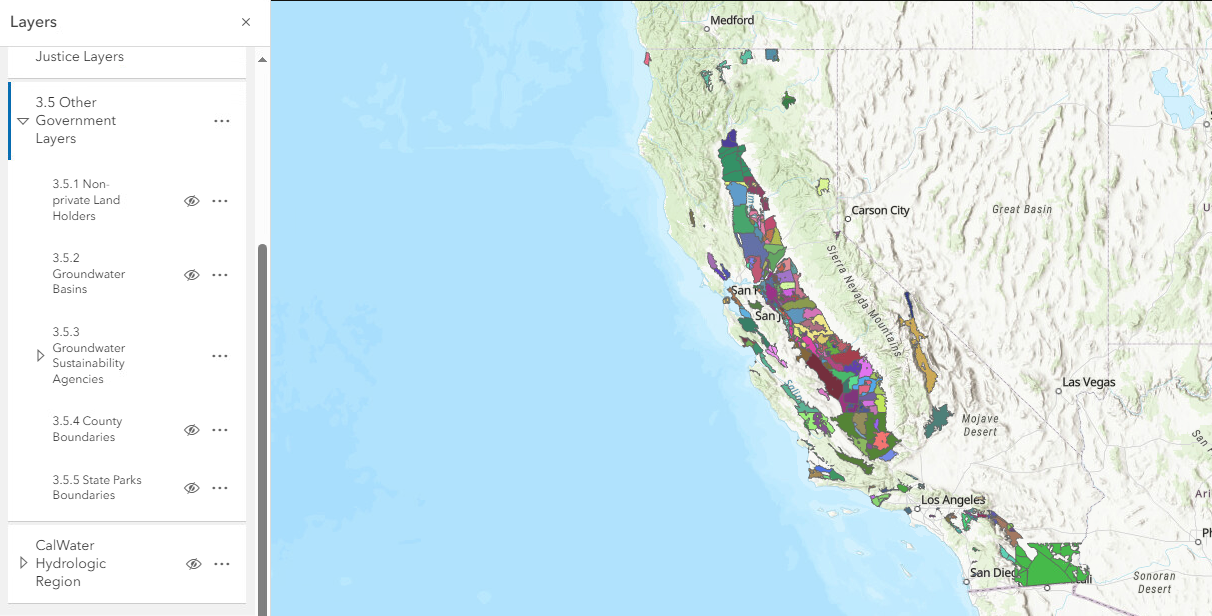
\includegraphics[keepaspectratio]{images/layer-guide-gsa-boundaries.png}}

Source:
\href{https://data.ca.gov/dataset/i08-b118-ca-groundwaterbasins/resource/0bb7282a-e0b1-452f-a364-da785911843e}{California
Department of Water Resources}, for use by
\href{https://www.waterboards.ca.gov/gama/}{Groundwater Ambient
Monitoring and Assessment (GAMA) Program}

Data Update Frequency: As needed

\subsection{Marine Protected Areas}\label{marine-protected-areas}

California's MPA Network includes different types of MPAs as well as
other designations. Each designation is unique in its purpose and
allowed uses -
\href{https://wildlife.ca.gov/Conservation/Marine/MPAs/About}{CDFW}

\ul{State Marine Reserve (SMP):} An MPA where no take, damage, injury,
or possession of any living, geologic, or cultural marine resource is
allowed.

\ul{No-Take State Marine Conservation Area (NoTake SMCA):} An MPA where
no take of any living, geologic, or cultural resource is allowed, EXCEPT
for take incidental to specified activities permitted by other agencies
(e.g.~infrastructure maintenance, sand renourishment).

\ul{State Marine Park (SMP)}: An MPA that allows some recreational take
but does not allow commerical take.

\ul{State Marine Conservation Area (SMCA)}: An MPA where some
recreational and/or commercial take of marine resources may be allowed
(restrictions vary)

\ul{State Marine Recreational Management Area (SMRMA)}: A marine managed
area where some take of marine resources may be allowed and legal
waterfowl hunting is allowed (restrictions vary)

\ul{Special Closure}: Prohibits or restricts access in waters adjacent
to seabird rookeries or marine mammal haul-out sites.

\emph{Screenshot here}

Source: \href{https://map.dfg.ca.gov/metadata/ds0582.html}{California
Marine Protected Areas {[}ds582{]} GIS Dataset}

Data Update Frequency: As needed

Last Updated: 2019

\bookmarksetup{startatroot}

\chapter{Resources}\label{resources}

Here you will find a curated list of presentations, webpages and other
resources related to the development, implementation and scaling of the
Water Board's Tribal Water Data Map.

All Water Boards authors are \textbf{bolded} below.

\section{Websites}\label{websites}

\href{https://www.waterboards.ca.gov/resources/oima/tribal_water_data_initiatives/}{Water
Boards' Tribal Water Data Initiatives}

\section{SWAMP Information}\label{swamp-information}

\begin{itemize}
\item
  The Surface Water Ambient Monitoring Program (SWAMP) unit falls within
  the OIMA at the State Water Resources Control Board
\item
  Below are resources directly from the SWAMP website that may be useful
  in addition to this map:

  \begin{itemize}
  \item
    \href{https://gispublic.waterboards.ca.gov/swamp-data/}{SWAMP Data
    Dashboard}
  \item
    \href{https://mywaterquality.ca.gov/safe-to-swim/content/interactive_map/index.html}{Safe
    to Swim Map}
  \item
    \href{https://www.waterboards.ca.gov/water_issues/programs/swamp/freshwater_cyanobacteria.html}{Freshwater
    Harmful Algal Bloom (FHAB) Program}
  \end{itemize}
\end{itemize}

\section{Presentations}\label{presentations}

\href{https://drive.google.com/file/d/1fJSZywbhhlgFK6H-LSwDVOmc_iJZEErZ/view?usp=sharing}{Using
California Water Board's Tribal Water Data Map to Understand Pollution
\& Climate in your Area}. Jan 2025. \textbf{Anna Holder}.
\href{https://tribalclimatehealth.org/tools-resources/data-development/}{National
Tribal Data Resilience Workgroup}.
\href{https://youtu.be/im4xqnCkJ90?si=j6hubFR5mtjhcI7y&t=793}{Recording}

\href{https://drive.google.com/file/d/11xj_Bj4m9MeaVkGYySrKZOR-KEZCJh9x/view?usp=sharing}{Using
California Water Board's Tribal Water Data Map to Understand Pollution
in your Area}. Oct 2023
(\href{https://tribalepa.com/2023-conference/}{Fall Tribal Conference}).
\textbf{Anna Holder}, Sarah Ryan. Tribal EPA \& US EPA Region 9 Annual
Conference.
\href{https://youtu.be/5s0AfEzw2_s?si=HAj_03DC3PDUnfHp&t=185}{Recording}

\href{https://docs.google.com/presentation/d/1-K_To1xSz9-GATblLJswJyQCUD0pcI1QFzAo591XVNk/edit?usp=sharing}{CA
Water Boards' Tribal Water Data Resources Update}. Aug 2023
(\href{https://www.epa.gov/tribal-pacific-sw/region-9-rtoc-meeting-materials-summer-2023}{Summer
Meeting}). \textbf{Badhia Yunes Katz}, \textbf{Anna Holder}. California
Issues Workgroup - US EPA Region 9 Regional Tribal Operations Committee
(RTOC).

\href{https://docs.google.com/presentation/d/1Xtgz76_KohNsLFq_sAtnEgPza8lrJs9CeJX2bvSngow/edit?usp=sharing}{Introduction
to CA Water Boards' Tribal Water Data Resources}. Feb 2023
(\href{https://www.epa.gov/tribal-pacific-sw/region-9-rtoc-meeting-winter-2023}{Winter
Meeting}). \textbf{Badhia Yunes Katz}, \textbf{Anna Holder}. California
Issues Workgroup - US EPA Region 9 Regional Tribal Operations Committee
(RTOC).

\section{Other Data Visualization
Tools}\label{other-data-visualization-tools}

\href{https://cawaterdatadive.shinyapps.io/ca-tribal-data/}{Tribal
Drinking Water} - This tool is intended to compile and display
information that can inform and help prioritize outreach related to
drinking water issues in tribal areas within California. It is a work in
progress, and is not intended to be a comprehensive source of
tribal-related water data.

\href{https://map.healthyplacesindex.org/?}{Healthy Places Index (HPI)}
- The HPI maps data on social conditions that drive health --- like
education, job opportunities, clean air and water, and other indicators
that are positively associated with life expectancy at birth. The HPI is
a project of the Public Health Alliance of Southern California, with the
aim of supporting efforts to prioritize equitable community investments
and policy.

\href{https://www.atsdr.cdc.gov/placeandhealth/svi/interactive_map.html}{Social
Vulnerability Index (SVI)} - The SVI is designed to identify and
quantify communities experiencing social vulnerability and help public
health officials and local planners better prepare for and respond to
emergency events. It is developed by the US Centers for Disease Control
and Prevention and Agency for Toxic Substances and Disease Registry.

\bookmarksetup{startatroot}

\chapter{Meet the Team!}\label{meet-the-team}

The development of the
\href{https://gispublic.waterboards.ca.gov/portal/home/item.html?id=a71c1841907240e1a4d896c8cf2302a8}{Map}
and this User Manual has been a team effort from the start. Below is a
list of team members within OIMA and tribal partners who have been
integral to the development of these resources.

If you would like to join the Team, please email Anna Holder at:
\href{mailto:anna.holder@waterboards.ca.gov}{\nolinkurl{anna.holder@waterboards.ca.gov}}.

\section{OIMA}\label{oima}

\begin{longtable}[]{@{}
  >{\raggedright\arraybackslash}p{(\linewidth - 2\tabcolsep) * \real{0.5000}}
  >{\raggedright\arraybackslash}p{(\linewidth - 2\tabcolsep) * \real{0.5000}}@{}}
\toprule\noalign{}
\begin{minipage}[b]{\linewidth}\raggedright
Name
\end{minipage} & \begin{minipage}[b]{\linewidth}\raggedright
Title
\end{minipage} \\
\midrule\noalign{}
\endhead
\bottomrule\noalign{}
\endlastfoot
\href{mailto:anna.holder@waterboards.ca.gov}{Anna Holder} & Open Data
Science, Equity \& Tribal Coordinator \\
Hannah Merges & 2025 California Sea Grant Fellow \\
\end{longtable}

\section{Tribal Partners}\label{tribal-partners}

\begin{longtable}[]{@{}
  >{\raggedright\arraybackslash}p{(\linewidth - 4\tabcolsep) * \real{0.3333}}
  >{\raggedright\arraybackslash}p{(\linewidth - 4\tabcolsep) * \real{0.3333}}
  >{\raggedright\arraybackslash}p{(\linewidth - 4\tabcolsep) * \real{0.3333}}@{}}
\caption{Tribal partners listed in ascending order by Affiliation. We
are appreciative and grateful for Meyo Marrufo and Shasta Gaughen who
invested time to provide us early feedback on the content of the
\href{https://www.waterboards.ca.gov/resources/oima/tribal_water_data_initiatives/}{Tribal
Water Data Initiatives Webpage}, the
\href{https://gispublic.waterboards.ca.gov/portal/home/item.html?id=a71c1841907240e1a4d896c8cf2302a8}{Tribal
Water Data Map}, and this
\href{https://cawaterboarddatacenter.github.io/tribal-water-data-map-manual/}{Manual}.}\tabularnewline
\toprule\noalign{}
\begin{minipage}[b]{\linewidth}\raggedright
Name
\end{minipage} & \begin{minipage}[b]{\linewidth}\raggedright
Title
\end{minipage} & \begin{minipage}[b]{\linewidth}\raggedright
Affiliation
\end{minipage} \\
\midrule\noalign{}
\endfirsthead
\toprule\noalign{}
\begin{minipage}[b]{\linewidth}\raggedright
Name
\end{minipage} & \begin{minipage}[b]{\linewidth}\raggedright
Title
\end{minipage} & \begin{minipage}[b]{\linewidth}\raggedright
Affiliation
\end{minipage} \\
\midrule\noalign{}
\endhead
\bottomrule\noalign{}
\endlastfoot
Sarah Ryan & Environmental Director & Big Valley Band of Pomo Indians,
Environmental Protection Department
(\href{https://www.bvrancheria.com/epa}{Big Valley EPA}) \\
Meyo Marrufo & Former Environmental Director & Guidiville Rancheria \\
Shasta Gaughen & Director & Pala Band of Mission Indians, Environmental
Department (\href{http://ped.palatribe.com/}{PED}) \\
\end{longtable}

We also regularly receive critical feedback from the California Issues
Workgroup of the US EPA Region 9 Regional Tribal Operations Committee
(\href{https://www.epa.gov/tribal-pacific-sw/regional-tribal-operations-committee-rtoc}{RTOC}).
See the
\href{https://cawaterboarddatacenter.github.io/tribal-water-data-map-manual/resources.html}{Resource
Chapter} of this User Manual for past presentations.

\section{Former OIMA Fellows}\label{former-oima-fellows}

\begin{longtable}[]{@{}lll@{}}
\toprule\noalign{}
Name & Title & Fellowship Period \\
\midrule\noalign{}
\endhead
\bottomrule\noalign{}
\endlastfoot
Kevin Song & Stanford Fellow & Summer 2024 \\
Daly Wettermark & Stanford Fellow & Summer 2024 \\
Leah Benton & CivicSpark Fellow & 2023-2024 \\
Josh Davenport & Stanford Fellow & Summer 2023 \\
Badhia Yunes Katz & CivicSpark Fellow & 2022-2023 \\
\end{longtable}

\bookmarksetup{startatroot}

\chapter{Contributing}\label{contributing}

\section{Who can contribute}\label{who-can-contribute}

Currently, only members of the OIMA Team are able to make \emph{edits}
to this User Manual and the Map, however we are always looking for
feedback!

\begin{tcolorbox}[enhanced jigsaw, breakable, title=\textcolor{quarto-callout-important-color}{\faExclamation}\hspace{0.5em}{We want your feedback!}, coltitle=black, colframe=quarto-callout-important-color-frame, opacitybacktitle=0.6, colback=white, opacityback=0, bottomrule=.15mm, colbacktitle=quarto-callout-important-color!10!white, leftrule=.75mm, bottomtitle=1mm, toptitle=1mm, toprule=.15mm, left=2mm, titlerule=0mm, arc=.35mm, rightrule=.15mm]

If you have recommendations for improvement related to the Map or this
User Manual you can send it to us by:

\begin{itemize}
\item
  Completing the \href{https://bit.ly/TWDM_Ideas}{Tribal Water Data Map
  Survey}, OR
\item
  Emailing Anna Holder at:
  \href{mailto:anna.holder@waterboards.ca.gov}{\nolinkurl{anna.holder@waterboards.ca.gov}},
  OR
\item
  Submitting a
  \href{https://github.com/CAWaterBoardDataCenter/tribal-water-data-map-manual/issues}{GitHub
  Issue}

  \begin{itemize}
  \tightlist
  \item
    Note this requires the individual to have a GitHub Account.
  \item
    If you would like to create a GitHub Account, complete Step 3 in the
    \href{https://cawaterboarddatacenter.github.io/tribal-water-data-map-manual/contribute.html\#setup}{Setup
    Section} below; no other steps need to be completed to submit an
    Issue.
  \end{itemize}
\end{itemize}

\end{tcolorbox}

\section{How we contribute at OIMA}\label{how-we-contribute-at-oima}

We develop the content for this User Manual using RStudio, build the
book using \href{https://quarto.org/}{Quarto} (via RStudio), and
collaborate and publish using GitHub (also via RStudio).

\subsection{Setup}\label{setup}

To contribute, OIMA Team members must do the following, and it should
only take about 20 minutes to complete:

\begin{enumerate}
\def\labelenumi{\arabic{enumi}.}
\item
  \textbf{Install R and RStudio}

  Both R and RStudio should be available in the Software Center (for
  Windows 10) or Company Portal (for Windows 11) -- if you don't see
  them in your Software Center/Company Portal or you have
  issues/questions during the installation process, please send a
  request to the DIT HelpDesk and they can help you install them.

  Also see these \href{https://www.r4wrds.com/intro/m_install_r}{step by
  step instructions on how to install these programs} -- you will only
  need to go through steps 1 and 2

  If you are new to R, it would also be helpful if you could review the
  \href{https://www.r4wrds.com/intro/m_getting_started.html}{Getting
  Started Module} so you can begin to familiarize yourself with the
  fundamentals of the program.
\item
  \textbf{Install Quarto}

  \href{https://quarto.org/docs/getting-started/installation.html}{Quarto
  download and install instructions}
\item
  \textbf{Create a GitHub Account}

  \href{https://docs.github.com/en/get-started/signing-up-for-github/signing-up-for-a-new-github-account}{Create
  your free personal account GitHub account}

  \href{https://happygitwithr.com/github-acct.html\#username-advice}{Tips
  on choosing your username}
\item
  \textbf{Download and Install Git}

  Follow your operating system's normal
  \href{https://git-scm.com/downloads}{Git installation process}. Note:
  you will not see an application called Git listed but if the
  installation process completed it was likely successful, and we will
  confirm together.
\end{enumerate}




\end{document}
